\documentclass{article} 
\UseRawInputEncoding
\usepackage[utf8]{inputenc}
\usepackage[T1]{fontenc}
\usepackage{selinput}
\usepackage[spanish]{babel}
\usepackage{hyphenat}
\usepackage{graphicx} 
\usepackage{subcaption}
\usepackage{hyperref}
\usepackage{listings}
\usepackage{xcolor}
\usepackage{float}
\usepackage[a4paper, total={6in, 9in}]{geometry}
\SelectInputMappings{%
  eacute={é},
}

\definecolor{codegreen}{rgb}{0,0.6,0}
\definecolor{codegray}{rgb}{0.5,0.5,0.5}
\definecolor{codepurple}{rgb}{0.58,0,0.82}
\definecolor{backcolour}{rgb}{0.95,0.95,0.92}

\lstdefinestyle{mystyle}{
    backgroundcolor=\color{backcolour},
    commentstyle=\color{codegreen},
    keywordstyle=\color{blue},
    numberstyle=\tiny\color{codegray},
    stringstyle=\color{codepurple},
    basicstyle=\ttfamily\footnotesize,
    breakatwhitespace=false,
    breaklines=true,
    captionpos=b,
    keepspaces=true,
    numbers=left,
    numbersep=5pt,
    showspaces=false,
    showstringspaces=false,
    showtabs=false,
    tabsize=2
}

\lstdefinelanguage{CSS}{
  keywords={color,background-image:,margin,padding,font,weight,display,position,top,left,right,bottom,list,style,border,size,white,space,min,width, transition:, transform:, transition-property, transition-duration, transition-timing-function},	
  sensitive=true,
  morecomment=[l]{//},
  morecomment=[s]{/*}{*/},
  morestring=[b]',
  morestring=[b]",
  alsoletter={:},
  alsodigit={-}
}
\lstset{style=mystyle}
\date{} 

\begin{document} 

\begin{center}
    
\includegraphics[width=1\textwidth]{Images/Imagenes/logo/LogoBIASbn.png}\\ 
\end{center}
    
\title{BIAS} 

\vspace{1cm} 

\textbf{Integrantes del Proyecto:} 

\begin{itemize}
    \item Adell, Nicolas Fabian
    \item De Blasi, Luca
    \item Diaz Melion, Danilo Sebastian
    \item Gil Soria, Ian Lucas
    \item Montenegro, Luciano Nahuel
    \item Sojka, Santiago Alejandro
\end{itemize}

\tableofcontents 

\newpage 

\section{Introducción}

BIAS es un módulo aplicable a una silla de ruedas que permite a los usuarios dirigirla mediante sus pensamientos, eliminando la necesidad de controles físicos tradicionales y optimizando la experiencia de movilidad. Este proyecto representa un avance significativo en el campo de la movilidad asistida, con el objetivo de mejorar la independencia y la calidad de vida de las personas con movilidad reducida.

Este sistema se basa en la avanzada tecnología de interfaz cerebro-computadora (BCI), la cual captura las señales neuronales del usuario y las traduce en comandos precisos para maniobrar la silla de ruedas sin esfuerzo. Además, el diseño modular y adaptable del sistema permite su integración en diversos modelos de sillas de ruedas y su personalización según las necesidades específicas de cada usuario. 

La seguridad es una prioridad fundamental en este desarrollo, por lo que el módulo incorpora múltiples capas de redundancia y verificación de señales, asegurando que la silla de ruedas responda de manera precisa y confiable a las intenciones del usuario. 

Aspiramos a revolucionar la forma en que las personas con movilidad reducida interactúan con su entorno, brindándoles una herramienta que amplía su capacidad para controlar su vida de manera más segura e independiente.

\subsection{Resumen del proyecto}
Este proyecto se centra en el desarrollo de una silla de ruedas controlada mediante señales cerebrales. El sistema se compone principalmente de los siguientes componentes: la silla de ruedas, un dispositivo EEG (electroencefalografo) y dos motores que permiten al usuario moverse en la dirección deseada.

El funcionamiento del sistema es el siguiente: el usuario se sienta en la silla y se coloca el EEG en la cabeza. A continuación, el usuario piensa en la dirección en la que desea moverse, y los motores responden en consecuencia.

El EEG tiene la función de leer las señales cerebrales del usuario. Estas señales se clasifican en las categorías de alpha, beta, gamma, delta y theta, y luego se someten a un proceso de filtrado para eliminar cualquier ruido. Posteriormente, las señales filtradas son analizadas por una Inteligencia Artificial (IA) desarrollada por nuestro equipo, la cual identifica patrones para determinar si el usuario desea moverse o detenerse.

Además, la silla está equipada con un sistema de emergencia que se activa en caso de lecturas erróneas o la detección de obstáculos. Este sistema de emergencia está compuesto por ultrasónidos que detectan la presencia de obstáculos frente a la silla.

\subsection{Motivación}
Como estudiantes de séptimo año, buscamos desarrollar un proyecto con el fin de cumplir con el requerimiento horario de practicas profesionalizantes. Nuestra intención inicial fue encontrar el proyecto ideal en cuestiones de impacto social, enfocándonos en la mejora de la calidad de vida de aquellas personas con discapacidades. Bajo este marco, y tras una extensa investigación, proponemos crear un módulo aplicable a una silla de ruedas controlado mediante la actividad cerebral del usuario, utilizando tecnología de interfaces cerebro-computadora (BCI), para brindarles mayor autonomía, independencia y participación social.   Creemos que este proyecto tiene el potencial de transformar la vida de las personas con movilidad motora reducida debido a enfermedades como ELA, esclerosis múltiple o cuadriplejia, permitiéndoles controlar su propio movimiento y mejorar significativamente su calidad de vida.
\subsection{Objetivos}
El objetivo de este proyecto es desarrollar una silla de ruedas motorizada que pueda ser controlada por la actividad cerebral del usuario. Esto beneficiaría a las personas con discapacidades motoras severas para lograr independencia y movilidad, mejorando su calidad de vida y participación en la sociedad. De esta manera, estas personas las cuales no pueden caminar o tienen movilidad reducida, pueden gozar de la utilización de una silla de ruedas controlada por señales cerebrales sin la utilización de ambas manos y meramente por sus pensamientos, dándole libertad y autonomía al usuario.

\section{¿Quiénes somos?}
Somos el grupo BIAS (Brain Intelligence Artificial System), conformado por seis estudiantes de la especialidad de Aviónica del séptimo año, segunda división, comisión C, de la Escuela Técnica N° 7 IMPA "Taller Regional Quilmes". Nuestro equipo se encuentra comprometido en el desarrollo de un módulo adaptable para sillas de ruedas, para así poder brindarles mas independencia y movilidad.
\subsection{Contactos}

En este apartado se detallarán los contactos a los integrantes del proyecto, adjuntando enlaces a sus redes:

\subsubsection{Adell Nicolás}

\begin{minipage}[t]{0.3\textwidth}
\begin{figure}[H]
    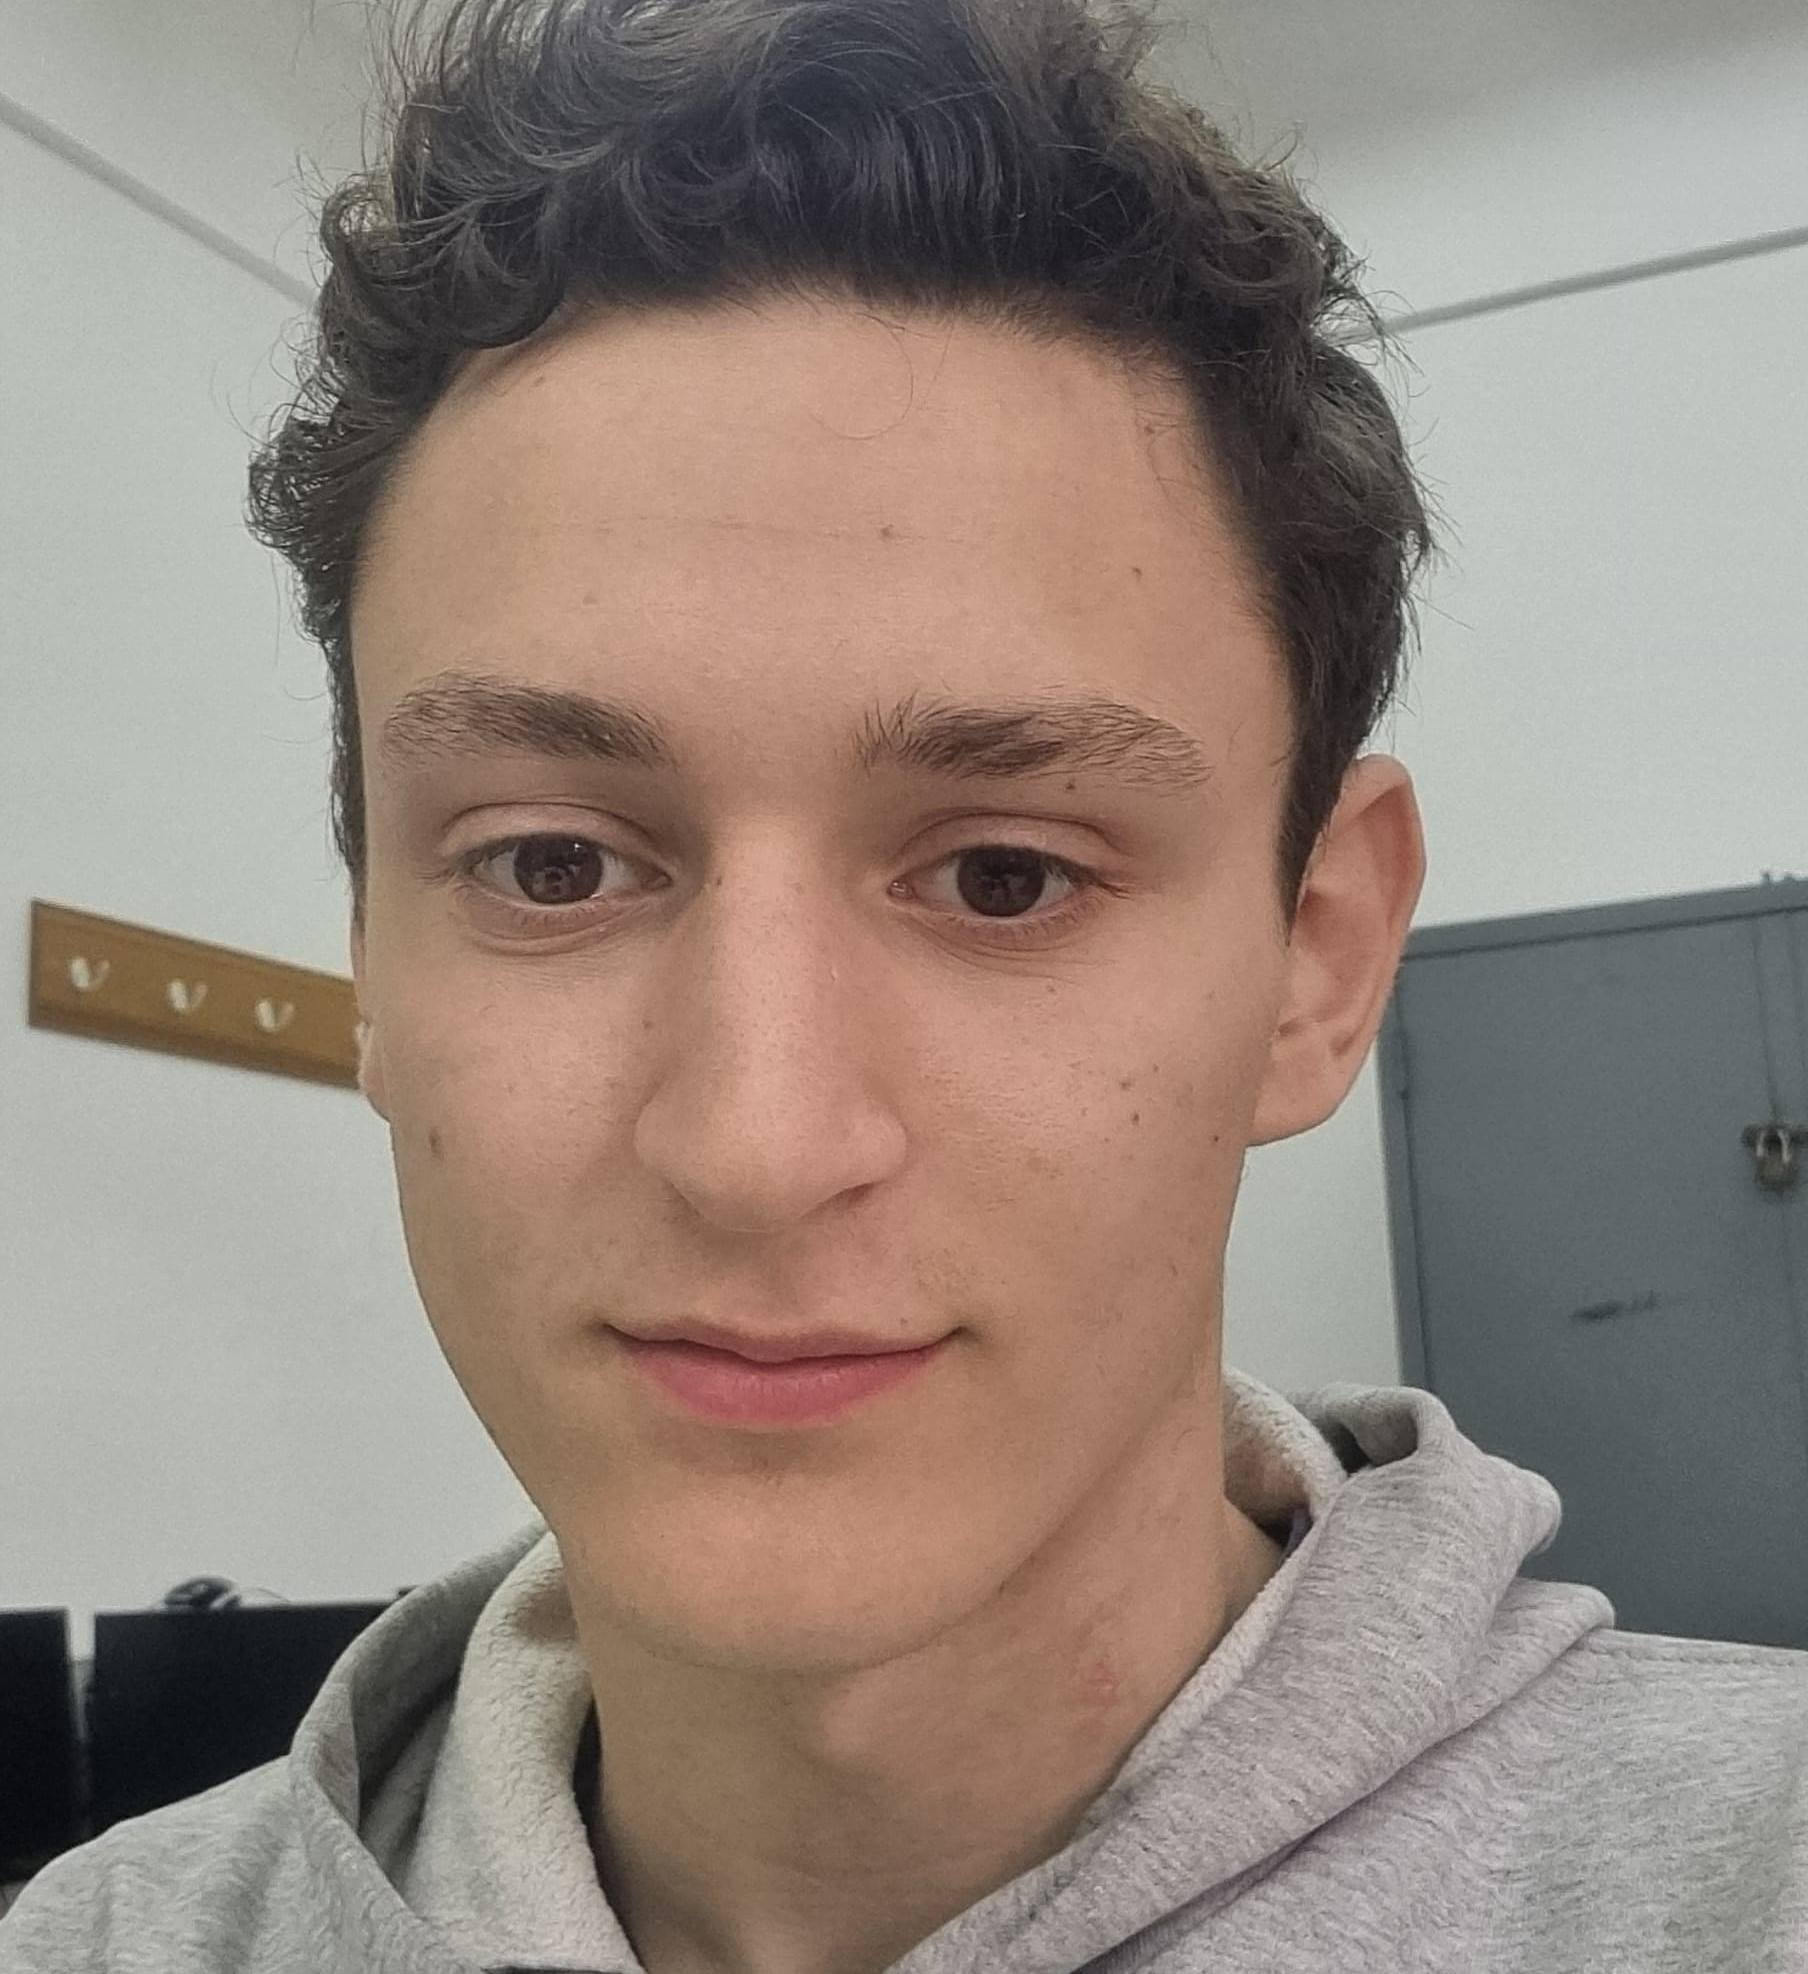
\includegraphics[width=0.75\linewidth]{Images//Personas/Fabi.jpg}
\end{figure}
\end{minipage}
\begin{minipage}[t]{0.5\textwidth}
    \vspace{3.5em}
    \href{https://instagram.com/nicolas.adell}{Instagram} \\[1em]
    \href{http://www.linkedin.com/in/nicolas-adell-354508297}{LinkedIn} \\[1em]
    \href{mailto:nicolas.fabian2005@gmail.com}{Gmail}
\end{minipage}%

\subsubsection{De Blasi Luca}

\begin{minipage}[t]{0.3\textwidth}

\begin{figure}[H]
    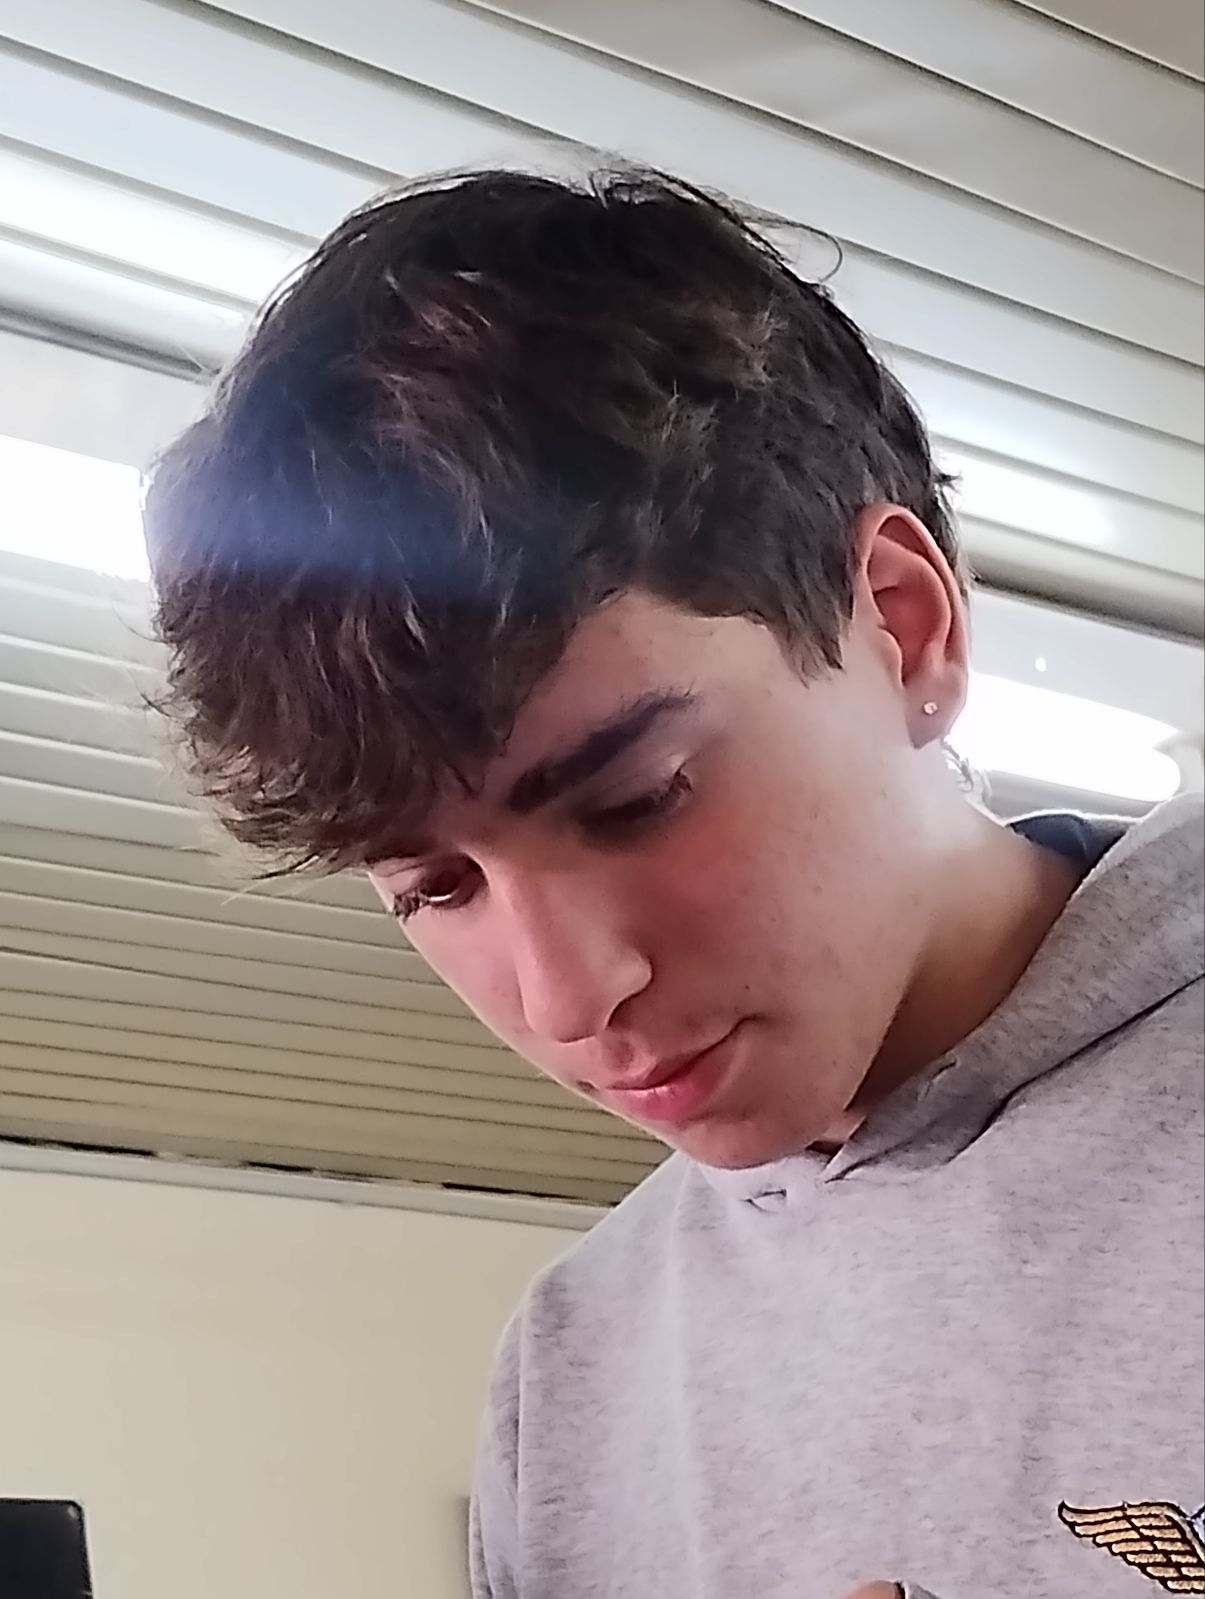
\includegraphics[width=0.75\linewidth]{Images//Personas/pela.jpg}
\end{figure}

\end{minipage}
\begin{minipage}[t]{0.5\textwidth}
    \vspace{3.5em}
    \href{https://instagram.com/luca.deblasii}{Instagram} \\[1em]
    \href{https://www.linkedin.com/in/luca-de-blasi-31164b304}{LinkedIn} \\[1em]
    \href{mailto:luqac2006@gmail.com}{Gmail}
\end{minipage}%

\subsubsection{Diaz Melión Danilo}

\begin{minipage}[t]{0.3\textwidth}

    \begin{figure}[H]
        
\includegraphics[width=0.75\linewidth]{Images//Personas/Dani.jpg}
    \end{figure}

\end{minipage}
\begin{minipage}[t]{0.5\textwidth}
    \vspace{3.5em}
    \href{https://instagram.com/_danilodiaz}{Instagram} \\[1em]
    \href{https://www.linkedin.com/in/danilodiazmelion/}{LinkedIn} \\[1em]
    \href{mailto:danilodiaz934@gmail.com}{Gmail}
\end{minipage}%

\subsubsection{Gil Soria Ian}
\begin{minipage}[t]{0.3\textwidth}

\begin{figure}[H]
    
\includegraphics[width=0.75\linewidth]{Images//Personas/Soria2.png}
\end{figure}

\end{minipage}
\begin{minipage}[t]{0.5\textwidth}
    \vspace{3.5em}
    \href{https://instagram.com/ian_gilsooor}{Instagram} \\[1em]
     \href{https://www.linkedin.com/in/ian-lucas-gil-soria-a8090b2a8?utm_source=share&utm_campaign=share_via&utm_content=profile&utm_medium=android_app}{LinkedIn} \\[1em]
    \href{mailto:ianlucasgilsoria@gmail.com}{Gmail}
\end{minipage}%

\subsubsection{Montenegro Luciano}
\begin{minipage}[t]{0.3\textwidth}

\begin{figure}[H]
    
\includegraphics[width=0.7\linewidth]{Images//Personas/Lucho.jpg}
\end{figure}

\end{minipage}
\begin{minipage}[t]{0.5\textwidth}
    \vspace{3.5em}
    \href{https://instagram.com/luchito_.montenegro}{Instagram} \\[1em]
    \href{https://www.linkedin.com/in/luciano-montenegro-3215aa304}{LinkedIn} \\[1em]
    \href{mailto:lucianomontenegro1021@gmail.com}{Gmail}
\end{minipage}%

\subsubsection{Sojka Santiago}
\begin{minipage}[t]{0.3\textwidth}
\begin{figure}[H]
    \includegraphics[width=0.75\linewidth]{Images//Personas/Sojka.jpg}
\end{figure}
\end{minipage}
\begin{minipage}[t]{0.5\textwidth}
    \vspace{3.5em}
    \href{https://instagram.com/sojkaa.sant}{Instagram} \\[1em]
    \href{https://www.linkedin.com/in/santiago-sojka-817198271/}{LinkedIn} \\[1em]
    \href{mailto:santiagosojka@gmail.com}{Gmail}
\end{minipage}%


\section{Desarrollo del Proyecto}
En este capítulo se expondrá en detalle la metodología empleada para avanzar en el desarrollo del proyecto, incluyendo las fuentes de inspiración y los proyectos similares que se tomaron como referencia para el diseño de nuestros circuitos y la programación de los sistemas. Además, se incluirán imágenes ilustrativas de estos proyectos de referencia, con el fin de ofrecer una comprensión visual más completa. Al finalizar el capítulo, se presentarán y explicarán los resultados obtenidos, evaluando su eficacia en relación con los objetivos planteados.

\subsection{Metodología}
La metodología aplicada en este proyecto se basa en la organización del equipo en dos grupos especializados. El primer grupo se encarga del desarrollo de los programas, siendo ejemplos de esto los filtros virtuales, programas de recepción y procesado, mientras que el segundo se dedica a la implementación de los motores, sistemas de emergencia y filtros. Esta división del trabajo permite una utilización más eficiente del tiempo, al abordar simultáneamente diversas áreas del proyecto, lo que resulta en un avance más significativo en periodos de tiempo más reducidos.


\subsection{Historia del Arte}
En este capitulo se repasa todos los conceptos previamente vistos mediante los cuales pudimos empezar a conceptualizar la idea del proyecto.

\subsubsection{Neuralink}
Uno de los casos que nos permitió aproximarnos a la conceptualización del proyecto fue el chip cerebral estilo implante de Neuralink, denominado Telepathy. Este dispositivo, desarrollado por la compañía de Elon Musk, tiene como objetivo facilitar la vida de las personas mediante la optimización de herramientas y su adaptación al cuerpo humano a través del implante. El chip crea una conexión entre el ser humano y dispositivos electrónicos, permitiendo, por ejemplo, controlar una puerta con traba eléctrica, desbloquear un teléfono móvil, e incluso monitorear el estado de ánimo de las personas.


Este ejemplo nos ofreció una perspectiva sobre la viabilidad de desarrollar un dispositivo, que, aunque no tan complejo, pudiera ser controlado por el propio cuerpo humano. A partir de esta premisa, iniciamos una investigación para explorar las posibilidades y opciones disponibles basadas en esta idea.


\subsubsection{Ryan Lopez EEG}
Si bien nuestro motivo y objetivo principal era crear un dispositivo original e innovador, también nos propusimos investigar proyectos con cierta similitud. En este proceso, encontramos el repositorio de un estudiante que desarrolló un sistema capaz de detectar señales alfa y, en función de las reacciones o pensamientos del usuario, permitir el control a través de un test de concentración. Este test consistía en que el usuario debía mantener un estado de concentración mientras estudiaba un documento para un examen, en lo que se podría considerar un simulacro.


El sistema desarrollado por Ryanlopezz activaba una alarma si los niveles de concentración del usuario comenzaban a disminuir, basándose en un espectro de señales alfa transmitidas por un conjunto de electrodos EEG dorados conectados a la cabeza del estudiante. Además, el sistema realizaba otras dos pruebas: una de ellas consistía en escribir en código Morse mediante pensamientos, enviando "pulsos de concentración", y la otra permitía controlar el movimiento de un personaje en el famoso videojuego "Flappy Bird", ajustando el impulso para subir o bajar.

En el siguiente link se adjunta la página de GitHub de Ryan Lopez en donde se puede observar más a detalle los programas y archivos de su EEG.


\begin{center}
    \href{https://github.com/ryanlopezzzz/EEG}{Ryan Lopez GitHub}
\end{center}


Gracias al mismo proyecto realizado por este usuario, pudimos desarrollar nuestro propio circuito para el sistema de filtrado, ya que íbamos a requerir otras especificaciones con diferentes funciones, tales como la entrada de señal: ya que esta debía ser mayor a la designada, al nosotros trabajar no solo con el espectro radioelectrico de las señales Alpha, sino con las principales señales que el cerebro produce al momento de realizar un pensamiento especifico; Por otro lado nosotros íbamos a requerir no solo un sistema de filtros EEG sino 4 placas del mismo circuito, debido a la posibilidad de maniobrar controlando los 3 ejes de los motores de la silla de ruedas


\begin{center}
    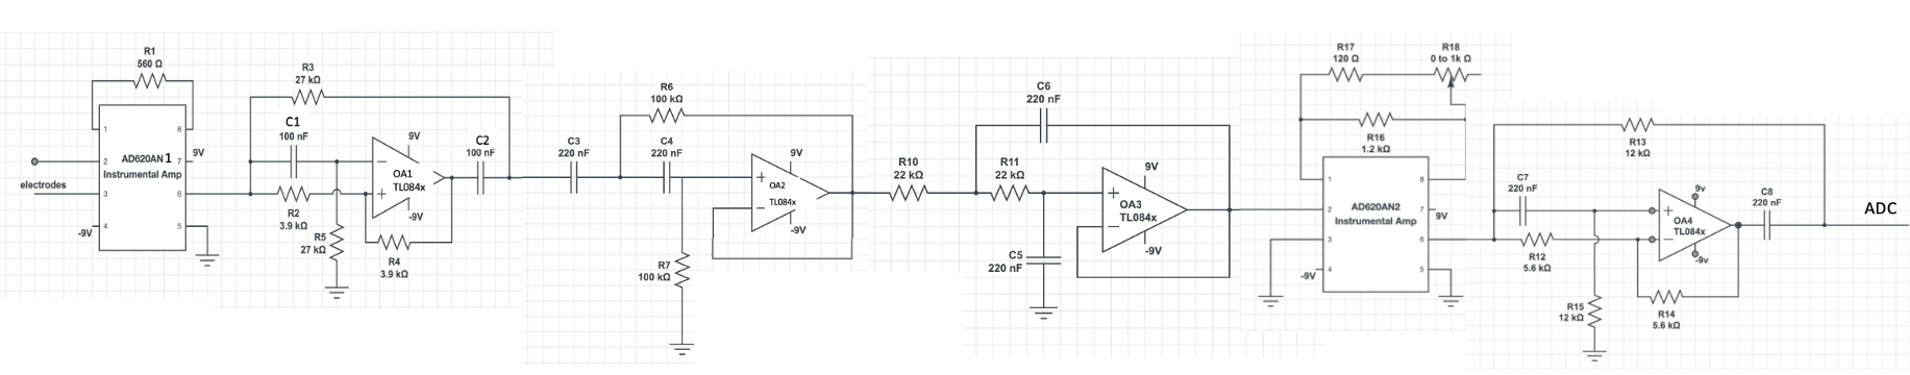
\includegraphics[width=1\textwidth]{Images/Imagenes/filtroeegderyan.png}\\
\end{center}

Por otro lado nos dio una primera vista de la localización de los botones EEG como irían colocados en la cabeza:

\begin{center}
    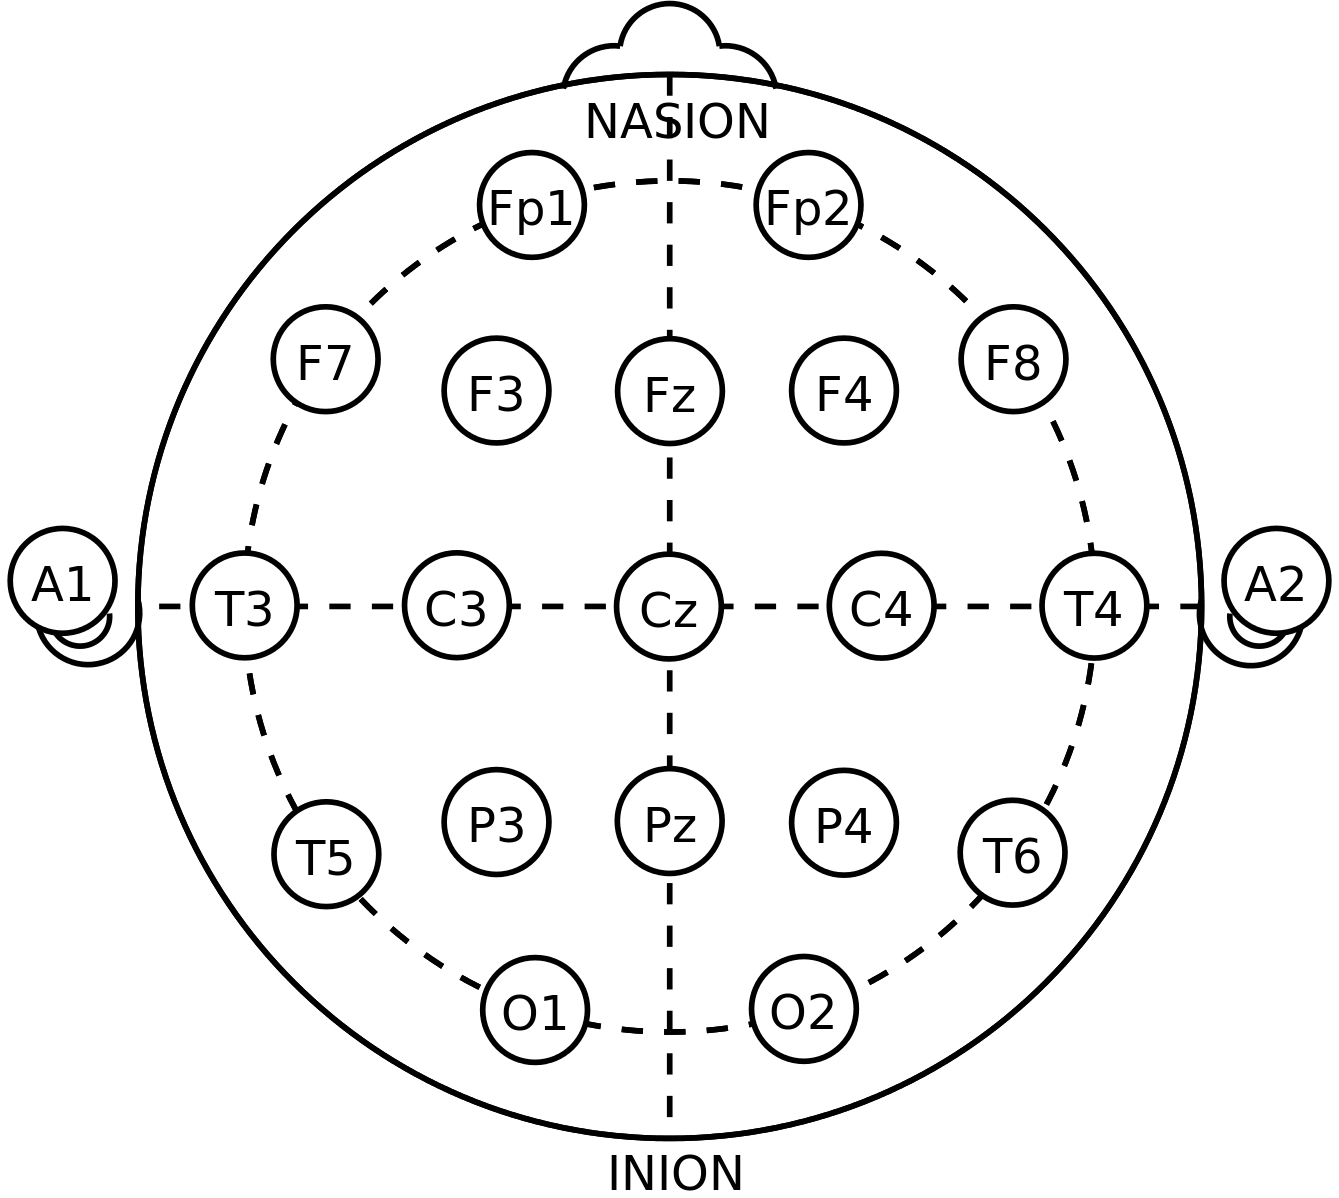
\includegraphics[width=0.85\textwidth]{Images/Imagenes/localizacionelectrodoseeg.png}\\

\end{center}

Así mismo para el estudio del aérea de medicina y saber como el cerebro humano se encarga de transmitir ciertas señales eléctricas gracias a la actividad cerebral  tuvimos en cuenta los actuales dispositivos de eneflografos, como se componen y actúan gracias ala actividad cerebral, bajo un especto radioelectrico determinado adjunto a la clasificación de las ondas transmitidas por el cerebro humano

\subsubsection{OpenBCI}

En nuestra búsqueda de conexiones para un microcontrolador y formas de desarrollar nuestro propio proyecto, descubrimos un sitio web llamado OpenBCI, una compañía especializada en la creación de dispositivos que integran tecnología con la interfaz del cuerpo humano. Esta empresa ha desarrollado un encefalógrafo casero, proporcionando dimensiones y parámetros estructurales que nos permitieron diseñar nuestra propia vincha/casco. Este dispositivo incorpora electrodos EEG, adaptados a la cabeza del usuario, como parte fundamental de nuestro proyecto "BIAS".

\begin{center}
    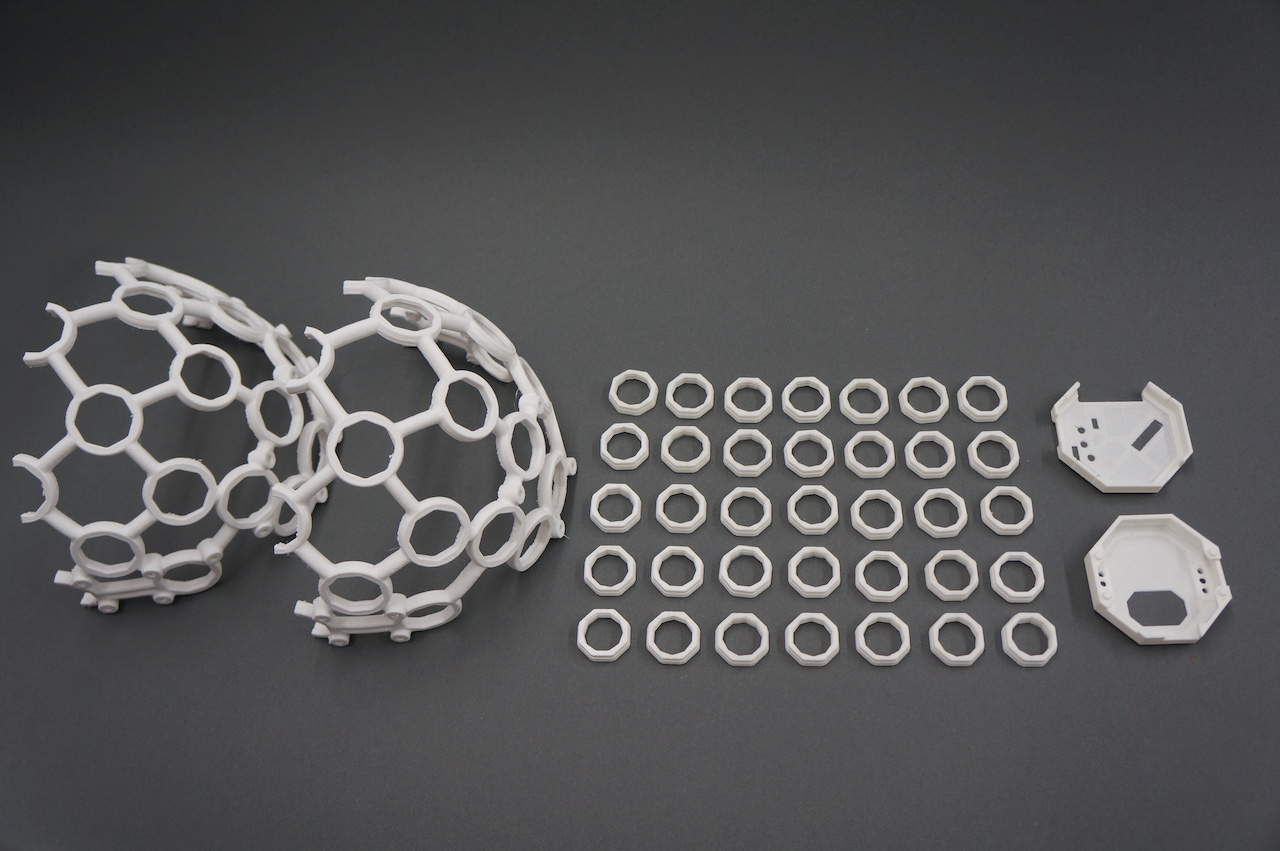
\includegraphics[width=1\textwidth]{Images/Imagenes/vinchamarkiv.png}\\
\end{center}

Además, al ser una compañía especializada en la creación de módulos de microcontroladores, nos proporcionaron orientación en cuanto a cómo realizar las conexiones entre la Raspberry Pi 4 que utilizamos y el sistema de filtrado EEG.

En los siguientes textos se adjuntan enlaces para ver la página oficial de OpenBCI y documentación de referencia correspondiente.

\begin{center}
    \href{https://openbci.com/}{Página oficial de OpenBCI}

    
    \href{https://docs.openbci.com/}{Documentación}

    
\end{center}

\begin{figure}[h!]
\centering

\begin{subfigure}[b]{0.45\linewidth}
    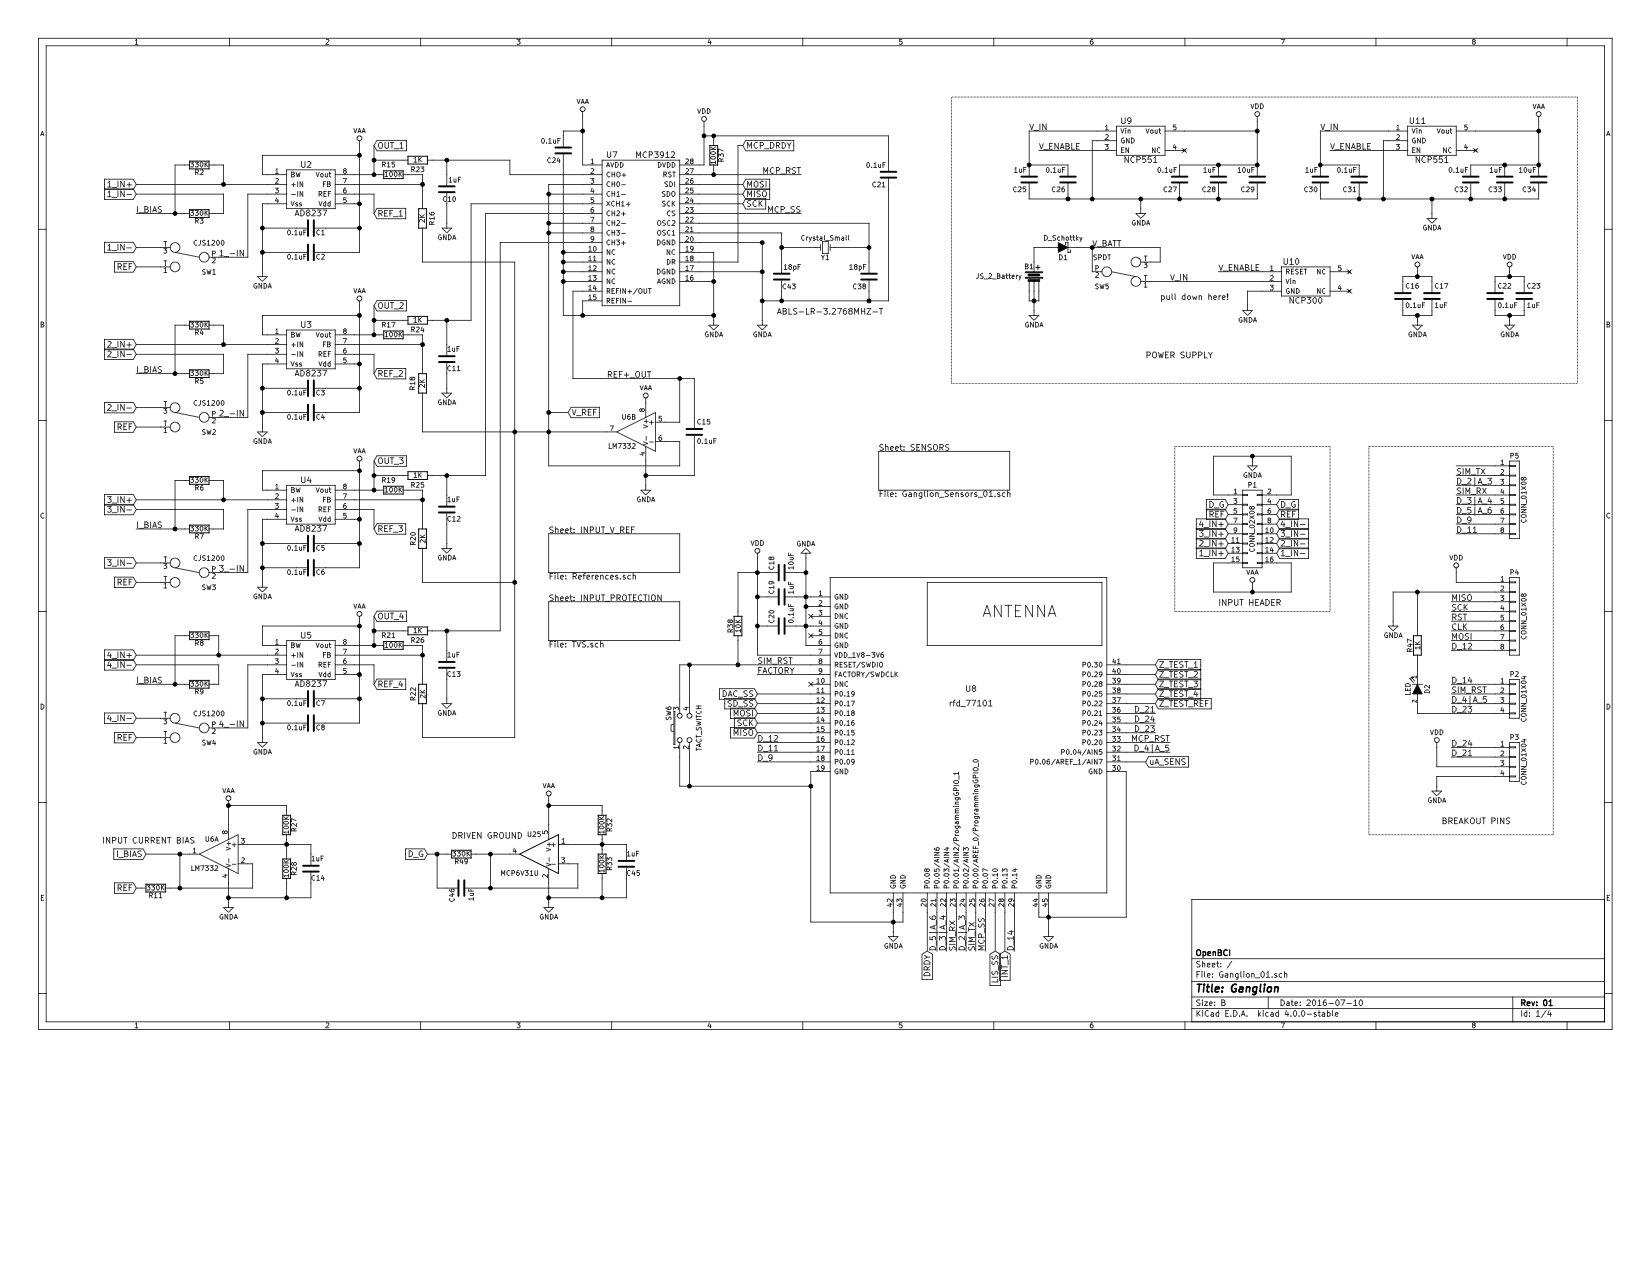
\includegraphics[width=\linewidth]{Images/Imagenes/esquematicodeganglion.png}
    \caption{Diseño Esquemático}
    \label{fig:westminster_lateral}
\end{subfigure}

\begin{subfigure}[b]{0.45\linewidth}
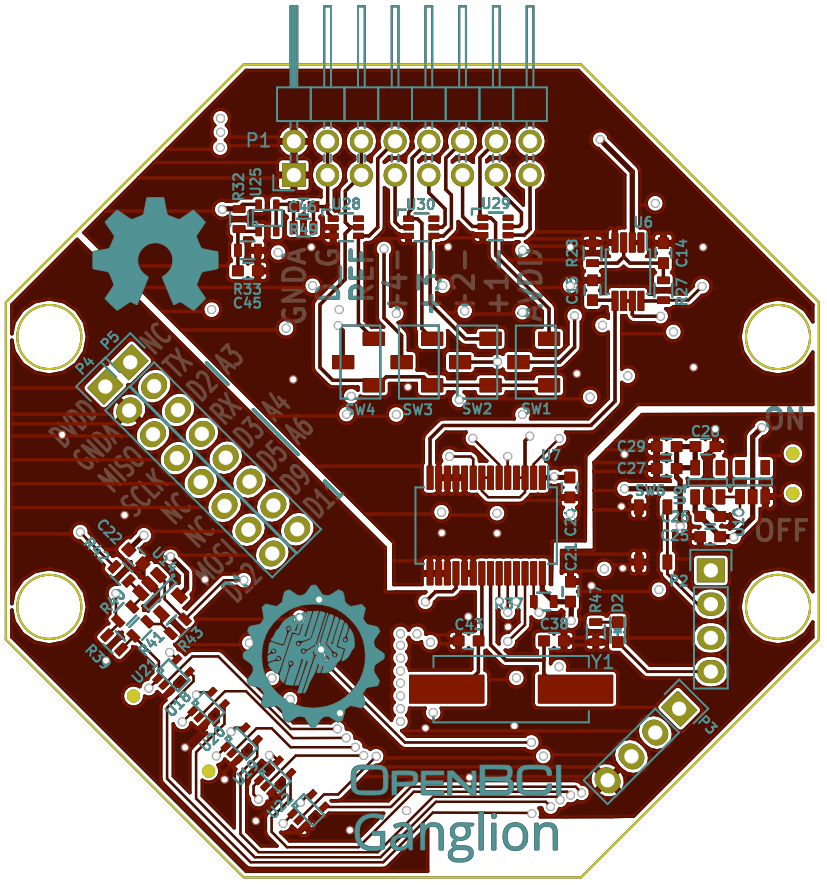
\includegraphics[width=\linewidth]{Images/Imagenes/pcbdeganglion.png}
\caption{Diseño PCB}
\label{fig:westminster_aerea}

\end{subfigure}
\caption{Diseño de microcontrolador de Open BCI}
\label{fig:westminster}
\end{figure}

\begin{center}
    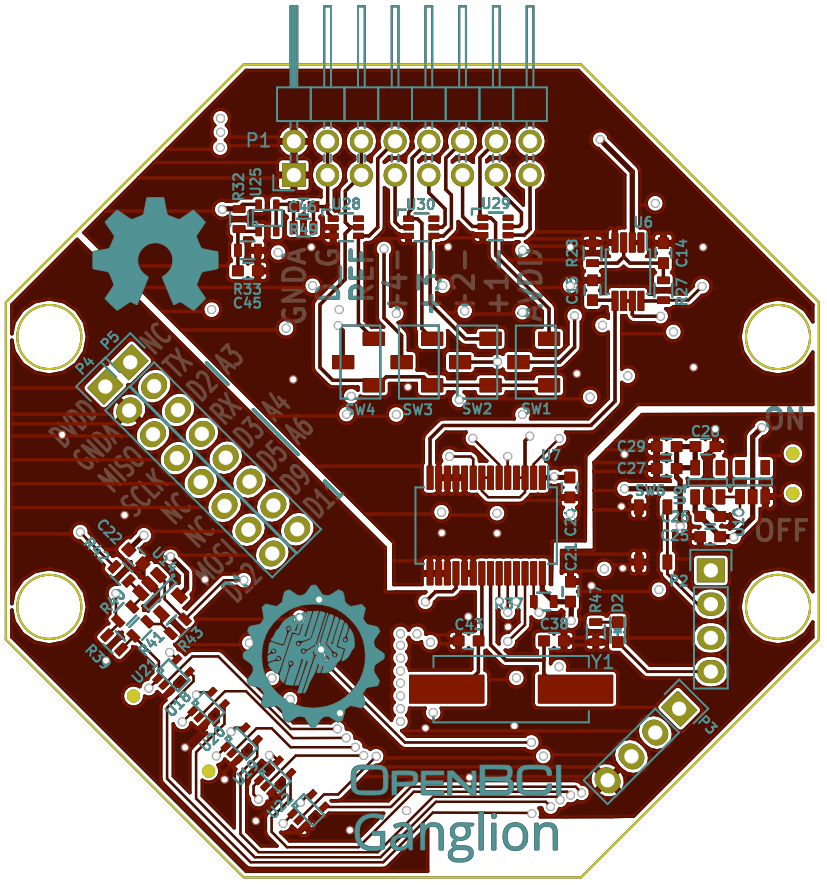
\includegraphics[width=0.5\textwidth]{Images/Imagenes/pcbdeganglion.png}\\

    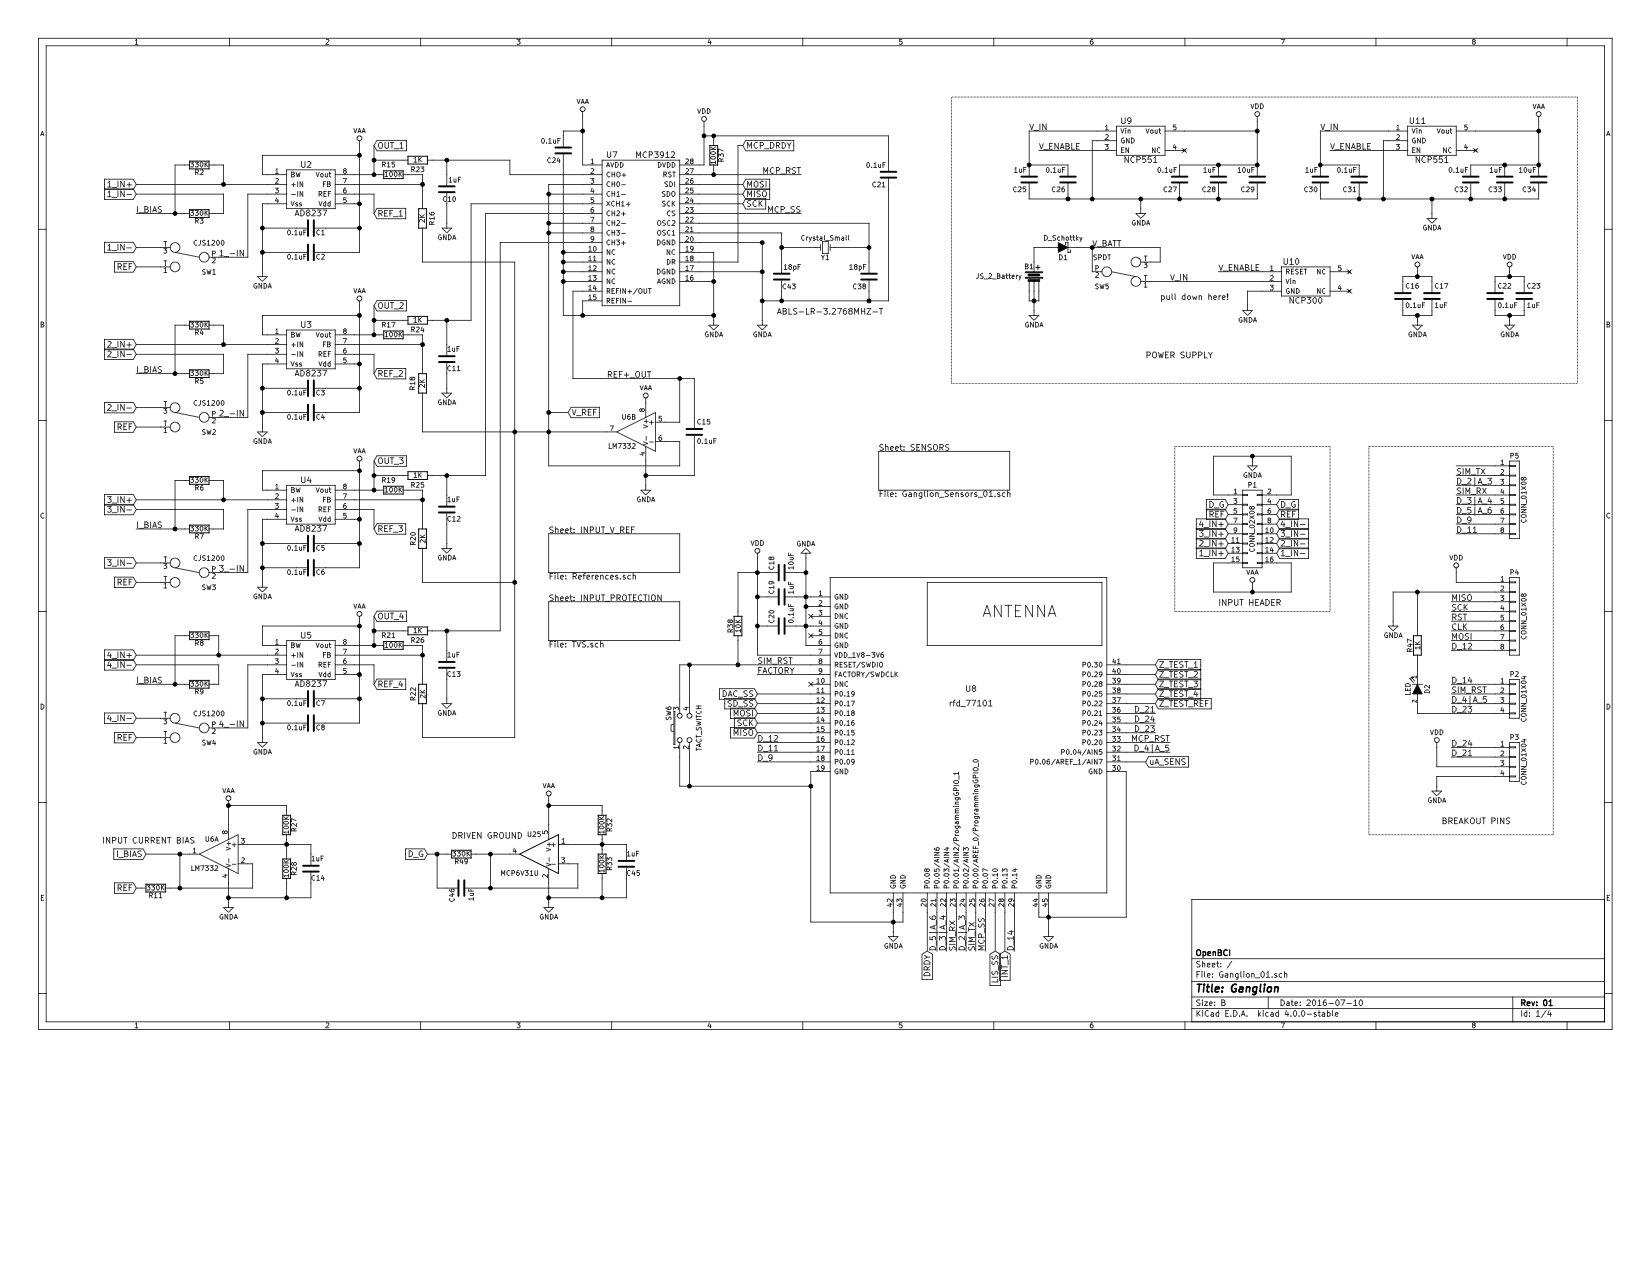
\includegraphics[width=1\textwidth]{Images/Imagenes/esquematicodeganglion.png}\\
\end {center}

\subsubsection{Autodesk Instructables}
A partir de esta página, obtuvimos los primeros circuitos necesarios para el EEG, lo que nos permitió avanzar de manera significativa en el desarrollo del proyecto. Esta fuente de información fue fundamental para sentar las bases técnicas y nos brindó las herramientas necesarias para continuar con el diseño y la implementación del sistema.

\section{Desarrollo Teórico}
En este capítulo se describirán y desarrollarán todos los aspectos teóricos relacionados, justificando la elección de los componentes utilizados. Se abordarán teorías como la Jaula de Faraday y el sistema 10-20, además de ofrecer una explicación detallada sobre los tipos de señales empleadas, entre otros temas relevantes.

\subsection{Distinción de alimentaciones}

En la etapa de recepción de señales provenientes de los electrodos, se empleará una fuente de alimentación compuesta por baterías de 9 voltios. La elección de este tipo de alimentación responde a la necesidad de limitar la corriente en caso de que ocurra algún problema en el circuito, previniendo así posibles daños a los componentes electrónicos. Esta misma fuente de alimentación será utilizada para suministrar energía a la placa de offset, asegurando que todos los subsistemas relacionados con la recepción de señales operen bajo condiciones controladas y seguras.

Para la alimentación del microcontrolador RP2040 Zero, se utilizará un regulador de 5 voltios que se encargará de convertir el voltaje de 9 voltios a un nivel más adecuado de 5 voltios, garantizando el correcto funcionamiento del dispositivo. La estabilidad en el suministro de voltaje es crucial en este tipo de sistemas, ya que cualquier fluctuación podría interferir con el procesamiento de las señales cerebrales y comprometer la precisión del sistema de control. Además, las distintas fuentes de alimentación están equipadas con condensadores conectados entre el terminal positivo y GND (tierra), con el objetivo de reducir las fluctuaciones en la tensión y minimizar la introducción de ruido en las señales. El ruido eléctrico, especialmente en sistemas de control y medición sensibles, puede degradar significativamente el rendimiento y la fiabilidad de los datos procesados.

El sistema de control de la silla de ruedas se alimentará mediante una batería de 24 voltios, la cual también suministrará energía al puente H y a los motores responsables del movimiento. Para garantizar la separación adecuada entre las distintas partes del sistema, se utilizará una masa adicional junto con un optoacoplador, que permitirá aislar eléctricamente la etapa de control de la etapa de potencia. Este desacoplamiento es esencial para evitar interferencias entre las señales de control y las corrientes más elevadas que circulan en el circuito de potencia.

Dentro del sistema de control, la Raspberry Pi 4 será alimentada mediante un regulador de 15 voltios, seguido de un segundo regulador que reducirá la tensión a 5 voltios. Este enfoque escalonado para la regulación del voltaje permite una mayor estabilidad en el suministro de energía, mejorando la eficiencia del sistema. De igual manera, se emplearán condensadores conectados en paralelo para reducir las posibles fluctuaciones de tensión y evitar la introducción de ruido, asegurando que la Raspberry Pi 4 funcione de manera óptima. La reducción del ruido es particularmente importante en sistemas basados en señales cerebrales, donde incluso pequeñas perturbaciones pueden alterar los resultados del procesamiento de señales EEG.

Finalmente, el puente H recibirá la alimentación directamente de la batería de 24 voltios. Para mantener una separación adecuada entre la etapa de control y la etapa de alimentación de los motores, se integrará otro optoacoplador, que garantizará que ambas secciones del circuito permanezcan eléctricamente aisladas. Sin embargo, aunque las masas de ambos sistemas no están directamente vinculadas en la placa, comparten el mismo punto de conexión en el borne de la batería de 24 voltios. Este diseño asegura que las distintas partes del sistema mantengan un nivel adecuado de aislamiento, mientras que las conexiones necesarias para la correcta operación del circuito se mantienen intactas.

\subsection{¿Que es un electroencefalograma?}

Un electroencefalograma (EEG) es una prueba médica que registra la actividad eléctrica del cerebro. Esta actividad se mide a través de electrodos colocados en el cuero cabelludo, que detectan las señales eléctricas generadas por las neuronas mientras se comunican entre sí. Estas señales eléctricas se representan como ondas cerebrales en una gráfica que muestra diferentes frecuencias y patrones.

El EEG se utiliza comúnmente para:
\begin{itemize}
    \item \textbf{Diagnóstico de trastornos neurológicos:} Como la epilepsia, convulsiones, trastornos del sueño, encefalopatías o daño cerebral.
    \item \textbf{Monitoreo del estado cerebral:} En procedimientos quirúrgicos, cuidados intensivos o investigaciones sobre coma y muerte cerebral.
    \item \textbf{Investigación neurológica y cognitiva:} Para estudiar la actividad cerebral en respuesta a estímulos externos, emociones o en procesos de toma de decisiones.
    \item \textbf{Interfaz cerebro-computadora (BCI):} Donde se usa para traducir la actividad cerebral en comandos para controlar dispositivos externos, como en tu proyecto de silla de ruedas controlada por EEG.
    
\end{itemize}

Las ondas cerebrales se clasifican en varios tipos según su frecuencia: delta, theta, alpha, beta, y gamma, cada una asociada a diferentes estados de conciencia y actividades cerebrales.

\begin{figure}[H]
    \centering
    \includegraphics[width=0.8\linewidth]{Images//EEG/EEG-waves.png}
    \caption{Vision de las Ondas Cerebrales en un electroencefalograma}
    \label{fig:enter-label}
\end{figure}

\subsection{¿Que es un EEG?}
Un electroencefalógrafo (EEG) es un dispositivo médico que se utiliza para registrar y medir la actividad eléctrica del cerebro. Su función principal es captar las señales eléctricas generadas por las neuronas y transformarlas en gráficos de ondas cerebrales, que se pueden analizar para evaluar la función cerebral, diagnosticar trastornos neurológicos y estudiar patrones de actividad cerebral. Las aplicaciones de los EEG incluyen investigaciones científicas, monitoreo clínico en neurocirugía, diagnóstico de epilepsia y el desarrollo de interfaces cerebro-computadora (BCI), como el control de dispositivos a través de señales cerebrales.

\subsubsection{Componentes que tiene un EEG:}
\begin{itemize}
    \item \textbf{Electrodos:} Son pequeños sensores colocados en el cuero cabelludo según el sistema internacional 10-20. Estos electrodos miden los cambios de voltaje producidos por la actividad eléctrica de las neuronas. Cada electrodo detecta la actividad en una región específica del cerebro, permitiendo un mapeo detallado de su actividad.
    \item \textbf{Amplificador:} Las señales eléctricas generadas por el cerebro son muy débiles, típicamente entre 0.5 a 100 μV. El amplificador del EEG aumenta estas señales, permitiendo que puedan ser procesadas y visualizadas. En algunos dispositivos avanzados, se utilizan técnicas de amplificación diferencial para mejorar la relación señal-ruido.
    \item \textbf{Conversor analógico-digital:} Las señales eléctricas captadas son analógicas, por lo que se requiere un conversor analógico-digital para traducirlas a un formato digital que pueda ser procesado por computadoras. La resolución del ADC es crítica, ya que define la precisión con la que las señales son capturadas.
    \item \textbf{Software de procesamiento:} El software realiza el filtrado y procesamiento de las señales crudas para eliminar el ruido o artefactos no relacionados con la actividad cerebral, como los generados por movimientos o interferencias eléctricas. Además, permite el análisis en tiempo real de las ondas cerebrales (Delta, Theta, Alpha, Beta, Gamma) y su interpretación para diversas aplicaciones, como estudios clínicos o interfaces cerebro-computadora.
    \item \textbf{Pantalla/Gráficos:}El electroencefalógrafo muestra las señales eléctricas como gráficos de ondas cerebrales. Estas ondas reflejan diferentes estados mentales, como relajación, concentración o sueño, y son analizadas por especialistas para determinar la actividad neurológica o la respuesta ante estímulos específicos.
\end{itemize}

\subsubsection{Aplicaciones del EEG}
\begin{itemize}
    \item \textbf{Diagnóstico clínico:} Es utilizado para diagnosticar y monitorear trastornos neurológicos como la epilepsia, trastornos del sueño, y diversas encefalopatías.
    \item \textbf{Investigación neurocientífica:} Permite estudiar los mecanismos del cerebro, la plasticidad cerebral, y las respuestas neuronales ante diversos estímulos.
    \item \textbf{Interfaces cerebro-computadora (BCI):} Las señales EEG pueden ser procesadas para controlar dispositivos, como sillas de ruedas eléctricas o prótesis, mediante la detección de patrones específicos de actividad cerebral.
    \item \textbf{Monitoreo intraoperatorio:} Durante cirugías neurológicas, el EEG puede utilizarse para monitorear la actividad cerebral en tiempo real y evitar daños en áreas críticas del cerebro.
\end{itemize}

\subsection{Cantidad de canales}
En el diseño de nuestra silla de ruedas controlada mediante señales cerebrales, hemos optado por un sistema de 4 canales con 9 electrodos (4 positivos, 4 negativos y 1 de masa) por varias razones clave, que refuerzan la precisión, la confiabilidad y la calidad de la señal capturada.

\begin{enumerate}
    \item \textbf{Optimización de la Captura de Señales EEG} 
    
    El cerebro humano emite diferentes tipos de ondas cerebrales (alfa, beta, gamma, delta y theta) que se distribuyen de manera no uniforme a lo largo del cuero cabelludo. Al utilizar 4 canales con 4 pares de electrodos (positivos y negativos) podemos capturar señales de distintas áreas cerebrales simultáneamente. Esto nos permite recoger información más completa y representativa de la actividad cerebral relevante para el control de la silla de ruedas.
    \item \textbf{Mayor Resolución en la Separación de Patrones Cerebrales} 
    
    El uso de múltiples electrodos garantiza una mayor resolución espacial en la detección de ondas cerebrales. Al disponer de 4 canales, podemos asociar cada canal a diferentes áreas de interés cerebral (como las regiones motoras o visuales), lo que aumenta la capacidad del sistema de IA para interpretar correctamente los patrones de ondas que se correlacionan con las intenciones de movimiento. Esto es crítico en una interfaz cerebro-computadora (BCI), donde la precisión es esencial para evitar errores en la dirección del movimiento.
    \item \textbf{Minimización de Ruido y Artefactos} 
    
    Cada par de electrodos está configurado en un modo diferencial, lo que nos ayuda a minimizar el ruido de fondo y los artefactos externos, como el ruido eléctrico del entorno o movimientos involuntarios. Los 4 electrodos negativos actúan como referencias de los positivos, de modo que la diferencia de potencial entre ellos permite eliminar parte del ruido que pudiera interferir en la calidad de la señal. Esto mejora considerablemente la relación señal/ruido y asegura una detección más precisa de las señales relevantes.
    \item \textbf{Uso del Electrodo de Masa para Estabilizar las Mediciones }
    
    El electrodo de masa se utiliza para estabilizar el sistema y reducir el ruido eléctrico residual. Este electrodo está conectado a un punto de referencia neutro, lo que permite estabilizar los potenciales medidos en los otros electrodos, asegurando que las fluctuaciones o interferencias no alteren la calidad de las señales EEG. La masa es esencial para la precisión global del sistema, evitando desequilibrios de voltaje que podrían provocar lecturas erróneas.
    \item \textbf{Equilibrio entre Complejidad y Procesamiento:}
    
    Optamos por 4 canales ya que representan un equilibrio adecuado entre complejidad técnica y capacidad de procesamiento. Más canales implicarían una mayor carga computacional para la Raspberry Pi 4, lo que podría requerir un hardware más potente o provocar retrasos en el procesamiento de las señales en tiempo real. Con esta configuración, logramos un sistema eficiente y suficiente para captar las señales necesarias sin comprometer la velocidad de respuesta del sistema de control de la silla.
    \item \textbf{Compatibilidad con el 'Sistema 10-20'} 
    
    La disposición de los electrodos sigue el estándar del 'Sistema 10-20' para garantizar una colocación uniforme y científicamente validada en el cuero cabelludo. Esto nos permite seleccionar puntos específicos que optimicen la captación de señales relevantes para nuestro sistema BCI, alineándonos con prácticas clínicas y de investigación que han demostrado ser efectivas en la medición de la actividad cerebral.
\end{enumerate}

El uso de estos filtros permite separar de manera efectiva las señales cerebrales del ruido presente en el entorno. Esto garantiza que las señales capturadas sean lo suficientemente limpias y precisas para su procesamiento por la Raspberry Pi 4. El diseño del sistema de filtrado incluye tanto filtros de paso bajo como de paso alto, optimizados para cada banda de frecuencia, lo que mejora la fiabilidad del control basado en las ondas cerebrales.

\subsection{Sistema 10-20}

El sistema 10-20 es un método internacionalmente estandarizado para la colocación de electrodos en el cuero cabelludo durante un electroencefalograma (EEG). Este sistema asegura que los electrodos se coloquen de manera uniforme y precisa en relación con los puntos anatómicos del cráneo, permitiendo una medición consistente y reproducible de la actividad eléctrica cerebral.

El nombre "10-20" proviene de las distancias porcentuales entre los electrodos: Los electrodos se colocan en posiciones que están al 10\% o al 20\% de la distancia total entre puntos anatómicos clave del cráneo.
Puntos anatómicos clave de referencia:
\begin{itemize}
    \item \textbf{Nasion:} El punto entre la frente y la nariz.
    \item \textbf{Inion:} El punto más prominente en la parte posterior de la cabeza.
    \item \textbf{Puntos preauriculares:} Justo por encima de los oídos, a cada lado de la cabeza.
\end{itemize}

Las posiciones de los electrodos se distribuyen sobre la cabeza tomando como referencia estos puntos para cubrir todo el cuero cabelludo de forma equidistante.

\begin{figure}[H]
    \centering
    \includegraphics[width=0.6\linewidth]{Images//Sistema_10-20/Sist-10-20.png}
    \caption{Puntos de medicion de Ondas Cerebrales}
    \label{fig:enter-label}
\end{figure}

\subsubsection{¿Para qué sirve?}
El sistema 10-20 se utiliza para garantizar una colocación precisa y consistente de los electrodos en los estudios de EEG. Algunos de sus beneficios incluyen:

\begin{itemize}

    \item \textbf{Estandarización global:} Permite que los estudios de EEG sean comparables en diferentes laboratorios y entre diferentes pacientes.
    \item \textbf{Cobertura completa del cerebro:} El sistema asegura que se cubran adecuadamente diferentes áreas del cerebro (frontal, parietal, occipital, temporal).
    \item \textbf{Detección de anomalías:} Facilita la identificación de regiones del cerebro donde pueden estar ocurriendo fenómenos anormales, como descargas epilépticas, actividad lenta anormal o asimetrías en las ondas cerebrales.
    
\end{itemize}

\subsubsection{¿Como se aplica?}

En un estudio de EEG, se colocan electrodos en el cuero cabelludo siguiendo estas posiciones predeterminadas en el sistema 10-20:

\begin{enumerate}
    \item Puntos y nomenclatura: Cada posición de electrodo tiene una nomenclatura que se utiliza para identificar las regiones del cerebro de las que se está registrando la actividad.
\end{enumerate}

\begin{itemize}
    \item F: Frontal (F3, F4, Fz, etc.)
    \item C: Central (C3, C4, Cz, etc.)
    \item P: Parietal (P3, P4, Pz, etc.)
    \item O: Occipital (O1, O2)
    \item T: Temporal (T3, T4, etc.)
    \item Los números impares (1, 3, 5, 7) se asignan al hemisferio izquierdo, mientras que los números pares (2, 4, 6, 8) se asignan al hemisferio derecho. La letra "z" indica posiciones centrales (a lo largo de la línea media de la cabeza).
\end{itemize}

\subsubsection{Pasos para aplicar el sistema 10-20}

\begin{enumerate}

    \item \textbf{Medición del cráneo:} Se mide la distancia desde el nasion al inion y desde un punto preauricular al otro. Luego, se calculan los puntos intermedios en un 10 o 20 de esas distancias para determinar las ubicaciones exactas de los electrodos.
    
    \item \textbf{Colocación de los electrodos:} Se colocan electrodos en los puntos marcados, asegurando una cobertura uniforme de la cabeza. Esto puede hacerse usando una gorra de EEG con posiciones ya marcadas o mediante la medición manual.
    
    \item \textbf{Registro de la actividad:} Una vez colocados los electrodos, se inicia el registro de la actividad cerebral. Los electrodos miden las diferencias de potencial eléctrico entre las regiones del cerebro cubiertas por los electrodos.
\end{enumerate}

\subsubsection{Aplicaciones del sistema 10-20}
\begin{itemize}
    \item \textbf{Diagnóstico clínico:} El sistema se usa comúnmente en estudios de EEG para diagnosticar condiciones neurológicas como la epilepsia, trastornos del sueño, y daño cerebral.
    \item \textbf{Investigación:} En estudios de neurociencia, el sistema 10-20 facilita la comparación de la actividad cerebral entre sujetos, ya que la ubicación de los electrodos está estandarizada.
    \item \textbf{Interfaces cerebro-computadora (BCI):} En proyectos de BCI, se utiliza el sistema 10-20 para colocar electrodos en áreas específicas del cerebro que controlan movimientos o funciones específicas.
\end{itemize}

\subsubsection{Colocacion de Electrodos}
Para llevar a cabo el registro de las señales EEG, es necesario disponer adecuadamente los electrodos. En nuestro proyecto, utilizamos un total de 9 electrodos, distribuidos en 4 canales: 4 electrodos positivos, 4 negativos y 1 de masa.

Los puntos de medición seleccionados para la colocación de los electrodos son los siguientes: Fp1, Fp2, F7, F8, T3, T4, O1, O2 y A2. Es importante señalar que los electrodos positivos se colocan en el lado derecho del cuero cabelludo (Fp2, F8, T4 y O2), mientras que los electrodos negativos se ubican en el lado izquierdo (Fp1, F7, T3 y O1). El electrodo de referencia o masa se posiciona en el lóbulo de la oreja, en el punto A2.

\subsection{Raspberry Pi 4}
La Raspberry Pi 4 es una computadora de bajo costo y tamaño compacto que se utiliza en una gran variedad de aplicaciones, especialmente en proyectos de electrónica, IoT (Internet of Things), y sistemas embebidos. Fue desarrollada por la Fundación Raspberry Pi para fomentar la educación en ciencias de la computación y se ha popularizado en proyectos de prototipado debido a su flexibilidad, potencia, y precio accesible.

\begin{figure}[H]
    \centering
    \includegraphics[width=0.8\linewidth]{Images//RPi4/rpi4-pinout.png}
    \caption{Raspberry Pi 4 PinOut}
    \label{fig:enter-label}
\end{figure}

\subsubsection{Caracteristicas de la RPi4}
\begin{itemize}
    \item \textbf{Procesador:} Broadcom BCM2711, quad-core Cortex-A72 (ARM v8) de 64 bits a 1.5GHz.
    \item \textbf{Memoria RAM:} Existen variantes con 2GB, 4GB y 8GB de RAM LPDDR4.
    \item \textbf{Puertos USB:} 2 puertos USB 3.0 y 2 puertos USB 2.0.
    \item \textbf{Conectividad:} Ethernet Gigabit, WiFi 802.11ac, Bluetooth 5.0.
    \item \textbf{Salidas de video:} Dos puertos micro-HDMI, capaces de soportar resoluciones 4K.
    \item \textbf{Almacenamiento:} No tiene disco duro interno, pero se utiliza una tarjeta microSD para almacenar el sistema operativo y los archivos.
    \item \textbf{Puertos GPIO:} 40 pines GPIO (General Purpose Input/Output) para conectar diversos componentes electrónicos, como sensores, actuadores y módulos de comunicación.
    \item \textbf{Alimentación:} Requiere una fuente de alimentación de 5V/3A mediante un puerto USB-C.
\end{itemize}

\subsubsection{Uso de la Raspberry Pi 4 en la silla}
Los pines GPIO de la Raspberry Pi 4 permiten interactuar con una variedad de componentes, como sensores, actuadores y módulos de comunicación. En nuestro proyecto, utilizamos estos pines para:

\begin{itemize}
    \item \textbf{Control de Motores:} A través de los pines GPIO, enviamos señales a los controladores de motores que ajustan la velocidad y dirección de los mismos, permitiendo los movimientos precisos de la silla de ruedas.
    \item \textbf{Recepción de Señales EEG:} Las señales EEG provenientes de los electrodos colocados en el cuero cabelludo se procesan con un convertidor ADC (convertidor de señal análoga a digital) y se envían a la Raspberry Pi para su análisis y clasificación en tiempo real.
    \item \textbf{Sistema de Emergencia:} La Raspberry Pi se encarga de controlar los sensores ultrasónicos ubicados en diferentes puntos de la silla de ruedas, activando LEDs y un buzzer cuando se detectan obstáculos en la trayectoria.
\end{itemize}

\subsubsection{Programacion con la RPi4}
La programación de la Raspberry Pi 4 se realiza principalmente en Python debido a su versatilidad y al soporte de bibliotecas específicas, como gpiozero, que facilita el control de los pines GPIO. En nuestro proyecto, Python se utiliza para las siguientes funciones:
\begin{itemize}
    \item \textbf{Procesamiento de Señales EEG:} Implementamos algoritmos que procesan las señales EEG en tiempo real utilizando filtros digitales y técnicas de análisis, como CAR (Common Average Reference) y ICA (Independent Component Analysis), para identificar los comandos que controlan la dirección de la silla.
    \item \textbf{Control de Motores y Sensores:} Se desarrolla un programa para controlar los motores y gestionar el sistema de emergencia, combinando datos de los sensores ultrasónicos con los comandos derivados de las señales EEG.
\end{itemize}
Gracias a su procesador de cuatro núcleos y opciones de memoria de hasta 8 GB, la Raspberry Pi 4 puede ejecutar múltiples tareas simultáneamente. Esto permite que el sistema realice el procesamiento de señales EEG, el control de motores y la gestión del sistema de emergencia sin interrupciones. Para maximizar la eficiencia, se han implementado técnicas de multithreading en el código, lo que permite que diferentes procesos se ejecuten en paralelo.

\subsubsection{Aplicaciones Generales de la RPi4}
Además de su uso en nuestro proyecto de silla de ruedas, la Raspberry Pi 4 tiene múltiples aplicaciones, entre las que se destacan:

\begin{itemize}
    \item \textbf{Automatización y Robótica:} Control de sistemas de robótica, como vehículos autónomos o robots, con la capacidad de gestionar múltiples sensores y motores simultáneamente.
    \item \textbf{Centros de Medios:} Configuración de servidores multimedia utilizando herramientas como Kodi, para la reproducción de videos y música.
    \item \textbf{IoT (Internet of Things):} Monitorización y control de dispositivos conectados a internet, como sistemas de seguridad, domótica y más.
    \item \textbf{Estaciones de Monitoreo:} Implementación de estaciones meteorológicas o de monitorización ambiental utilizando sensores conectados a los pines GPIO.
    \item \textbf{Proyectos Educativos:} Gracias a su bajo costo y la abundancia de recursos educativos, la Raspberry Pi es ideal para enseñar conceptos de programación, electrónica y robótica.
\end{itemize}

\subsection{Comunicación UART}

El UART (Universal Asynchronous Receiver-Transmitter) es un periférico de hardware utilizado para la comunicación serie. Su principal función es permitir la transmisión y recepción de datos de manera asíncrona, lo que implica que no requiere de una señal de clock compartida entre el transmisor y el receptor. A continuación, se destacan las características principales de este tipo de comunicación:

\begin{itemize}
    \item \textbf{Comunicación serie:} Los datos se transmiten de forma secuencial, bit a bit, a través de una línea de transmisión (TX) y se reciben mediante una línea de recepción (RX).
    \item \textbf{Asincronía:} Al no utilizar una señal de clock constante, ambos dispositivos deben estar configurados con la misma velocidad de transmisión (tasa de baudios) para asegurar la correcta recepción de los datos.
    \item \textbf{Formato de datos:} Cada paquete de datos transmitido generalmente incluye un bit de inicio (indicando el comienzo de la transmisión), entre 5 y 9 bits de datos, un bit opcional de paridad (para detección de errores), y uno o dos bits de parada.
    \item \textbf{Velocidad de transmisión:} La velocidad de transmisión de la información, conocida como tasa de baudios, se refiere al número de bits transmitidos por segundo.
\end{itemize}

La implementación de la comunicación UART en nuestro proyecto se utiliza para la recepción y procesamiento de señales. Específicamente, en la RP2040 Zero, enviamos las lecturas de los cuatro canales del ADC (Conversor Analógico-Digital) en formato JSON durante un período de tiempo definido y con una frecuencia de muestreo específica a la Raspberry Pi 4.

\begin{figure}[H]
    \centering
    \includegraphics[width=0.7\linewidth]{Images//UART/UART_Com.png}
    \caption{Comuniacion UART}
    \label{fig:enter-label}
\end{figure}

\begin{figure}[H]
    \centering
    \includegraphics[width=0.7\linewidth]{Images//UART/UART_pulse.png}
    \caption{Envio de datos de UART}
    \label{fig:enter-label}
\end{figure}

\subsection{Gráfico de Fourier}
El gráfico de Fourier está basado en la Transformada de Fourier (TF), que es una operación matemática que descompone una señal en sus componentes sinusoidales de diferentes frecuencias. Este método es especialmente útil para analizar señales periódicas y no periódicas.

La Transformada de Fourier dicta que: 

Dada una señal \textit{x(t)} en el dominio del tiempo, la transformada de Fourier \textit{X(f)} se define como:

\begin{figure}[H]
    \centering
    \includegraphics[width=0.5\linewidth]{Images//Formulas/FormulaFourier.png}
\end{figure}

\newpage
Donde:
\begin{itemize}
    \item \textit{x(t)} es la señal en el dominio del tiempo.
    \item \textit{X(f)} es la señal transformada en el dominio de la frecuencia.
    \item \textit{f} es la frecuencia (Hz).
    \item \textit{j} es la unidad imaginaria 
    \item $e^{-j2\pi ft}$ es la función compleja que representa la descomposición en sinusoides.

\end{itemize}

El gráfico de Fourier representa la magnitud o la fase de la transformada de Fourier. Este gráfico tiene dos componentes importantes:

\begin{enumerate}
    \item \textbf{Espectro de Magnitud:} Se representa gráficamente la magnitud de cada frecuencia presente en la señal. En el eje horizontal está la frecuencia \textit{f}, y en el eje vertical está la magnitud |\textit{X(f)}|, que indica cuánta energía o potencia de la señal está concentrada en esa frecuencia específica.

    \begin{equation}
        |X(f)| = \sqrt{Re(X(f))^2+Im(X(f))^2}
    \end{equation}
    
    \item \textbf{Espectro de Fase:} Indica el desfase de cada frecuencia con respecto a la señal original. En el eje horizontal también está la frecuencia \textit{f}, y en el eje vertical está el ángulo de fase \theta(f), $ que puede calcularse como:
    

    \begin{equation}
        \theta = tan^{-1} \left(\frac{Im(X(f))}{a}\right)
        \label{eq:1}
    \end{equation}
\end{enumerate}

\begin{figure}[H]
    \centering
    \includegraphics[width=0.8\linewidth]{Images//Fourier/Fourier_graph2.png}
    \caption{Grafico de Fourier}
    \label{fig:enter-label}
\end{figure}

\subsubsection{¿Para que sirve?}
El grafico de Fourier es una herramienta que sirve para analizar señales en el dominio de la frecuencia.
\newpage
\begin{enumerate}
    \item \textbf{Análisis de frecuencias:}
    \begin{itemize}
        \item \textbf{Descomposición de señales complejas:} Permite descomponer una señal en sus componentes de frecuencia individuales. Esto es útil cuando quieres saber qué frecuencias están presentes en una señal y su importancia relativa.
    
        \item \textbf{Identificación de frecuencias dominantes:} El gráfico te muestra cuáles son las frecuencias que más contribuyen a la señal original, lo que es esencial para entender fenómenos periódicos y patrones.
    \end{itemize}
    \item \textbf{Filtrado de señales:}
    \begin{itemize}
        \item \textbf{Diseño de filtros:} Si necesitas eliminar ruido o componentes no deseados de una señal, el gráfico de Fourier ayuda a identificar las frecuencias del ruido o interferencia. Luego puedes diseñar un filtro que elimine esas frecuencias.
    
        \item \textbf{Filtrado de bandas:} Puedes aplicar filtros pasa-bajas, pasa-altas o de banda (pasa-banda o elimina-banda) a una señal. El gráfico te muestra exactamente qué frecuencias están siendo afectadas.
    \end{itemize}
    
    \item \textbf{Compresión de datos:}
    \begin{itemize}
        \item \textbf{ Eliminación de información redundante:} En algunas señales (como imágenes o audio), las frecuencias más altas o muy bajas pueden no ser necesarias. Usando el gráfico de Fourier, puedes identificar esas frecuencias y eliminarlas para comprimir los datos sin perder información relevante.
    
        \item \textbf{Compresión de audio e imágenes:} Muchos algoritmos de compresión (como JPEG o MP3) utilizan la Transformada de Fourier o versiones discretas de ella para eliminar componentes de alta frecuencia que son menos perceptibles para el ser humano.
    \end{itemize}
    
    \item \textbf{Análisis de vibraciones y ondas:}
    \begin{itemize}
        \item \textbf{Detección de fallos en maquinaria:} En ingeniería mecánica y de control, el gráfico de Fourier es utilizado para analizar vibraciones y detectar problemas como desbalances, resonancias, o desgastes en partes móviles. Las frecuencias anómalas pueden señalar fallos.
    
        \item \textbf{Análisis de señales acústicas:} Permite estudiar el espectro de frecuencias en señales de audio. Por ejemplo, para identificar las características de sonidos musicales o voces.
    \end {itemize}
    
    \item \textbf{Procesamiento de señales EEG:}
    \begin{itemize}
        \item Para el análisis de señales cerebrales (EEG), el gráfico de Fourier es vital para identificar y separar las diferentes bandas de frecuencias asociadas con diferentes actividades cerebrales (como las ondas delta, theta, alpha, beta y gamma).
    
        \item \textbf{Monitoreo de actividad cerebral:} En neurociencia, el análisis de Fourier se utiliza para analizar patrones de actividad cerebral, detectar anormalidades y realizar interfaces cerebro-máquina (como el control de la silla de ruedas en tu proyecto).
    \end{itemize}
    \item \textbf{Análisis de señales en telecomunicaciones:}
    \begin{itemize}
        \item \textbf{Ancho de banda:} El gráfico de Fourier permite determinar el ancho de banda necesario para transmitir una señal sin pérdida de información.
    
        \item \textbf{Modulación y demodulación:} En sistemas de comunicaciones, la modulación de señales se realiza en el dominio de la frecuencia. El gráfico de Fourier te permite visualizar cómo una señal ha sido modulada para su transmisión y cómo se puede demodular para su interpretación.
    \end{itemize}
    \newpage
    \item \textbf{Análisis de imágenes:}
    \begin{itemize}
        \item \textbf{Reconocimiento de patrones:} En procesamiento de imágenes, la transformada de Fourier se utiliza para identificar patrones repetitivos o estructuras de frecuencia en una imagen. Es útil en tareas como la detección de bordes o compresión de imágenes.
    
        \item \textbf{Eliminación de ruido:} Permite eliminar patrones específicos de ruido en imágenes filtrando frecuencias indeseadas.
    \end{itemize}
\end{enumerate}

\subsubsection{¿En que lo aplicamos?}

Se emplea el Análisis de Fourier para identificar el espectro de frecuencias de las señales cerebrales, permitiendo la diferenciación de las ondas alpha, beta, gamma, delta y theta. Posteriormente, se aplica la Transformada Inversa de Fourier para reconstruir las señales en el dominio temporal, recuperando su forma original.

Una vez que las señales han sido diferenciadas por bandas de frecuencia, el algoritmo de machine learning procede a extraer las características (features) de cada tipo de onda a partir de una representación en el dominio de la frecuencia y del tiempo. Estas características son utilizadas para realizar la predicción del movimiento deseado en la silla de ruedas.

\subsubsection{¿Que es una feature?}

Una feature es una propiedad medible o una característica distintiva de un fenómeno. En el contexto de este proyecto, las features se refieren a las propiedades específicas de cada señal cerebral, clasificadas por tipo de onda (alpha, beta, gamma, delta y theta). Estas propiedades son extraídas para capturar la información relevante que permitirá al sistema de aprendizaje automático identificar patrones en las señales y realizar predicciones relacionadas con el control de la silla de ruedas.

\subsection{Filtros digitales}

Un filtro digital es una herramienta utilizada en el procesamiento de señales para modificar o mejorar ciertos aspectos de una señal digital, eliminando o atenuando componentes no deseados, como ruido, o destacando componentes útiles. Los filtros digitales operan sobre señales discretizadas (muestreadas) y utilizan algoritmos matemáticos para realizar diversas transformaciones.

Existen diferentes tipos de filtros digitales, según su función:

\begin{itemize}
    \item \textbf{Filtro pasa bajas:} Permite el paso de frecuencias bajas y atenúa las frecuencias altas.
    \item \textbf{Filtro pasa altas:} Permite el paso de frecuencias altas y atenúa las bajas.
    \item \textbf{Filtro pasa banda:} Permite el paso de un rango específico de frecuencias.
    \item \textbf{Filtro elimina banda (Notch):} Atenúa un rango específico de frecuencias, como en el caso de eliminar interferencias a 50-60 Hz.
\end{itemize}

Los filtros digitales pueden ser FIR (Finite Impulse Response) o IIR (Infinite Impulse Response):

\begin{itemize}
    \item Los filtros FIR tienen una respuesta finita y son más estables, pero pueden necesitar más recursos de procesamiento.
    \item Los filtros IIR tienen una respuesta infinita y suelen ser más eficientes en términos de recursos, pero pueden ser menos estables si no se diseñan correctamente.
\end{itemize}

Los filtros digitales son ampliamente usados en aplicaciones como procesamiento de audio, señales biológicas (como EEG), imágenes y telecomunicaciones.
\subsubsection{¿Para que los necesitamos si ya tenemos por Hardware?}
La combinación de filtros físicos (implementados en hardware) con filtros digitales (implementados en software) presenta una serie de ventajas significativas, incluso si ya se han instalado filtros físicos en el sistema. Aunque los filtros basados en hardware permiten un filtrado efectivo de las señales EEG, los filtros digitales proporcionan una flexibilidad y capacidades adicionales que no siempre son posibles de lograr mediante hardware exclusivamente. A continuación, se detallan las razones por las cuales puede ser beneficioso incorporar filtros digitales a la salida de los filtros físicos:
\begin{enumerate}
    \item \textbf{Ajuste Preciso y Mayor Flexibilidad}
    
    Los filtros de hardware están limitados a sus parámetros iniciales, ya que una vez construidos con componentes específicos (como resistencias, condensadores, etc.), sus características clave, tales como la frecuencia de corte y el ancho de banda, son difíciles de modificar. En contraste, los filtros digitales permiten ajustar fácilmente parámetros como la frecuencia de corte o la configuración de filtrado sin necesidad de realizar cambios físicos. Esto resulta especialmente útil cuando, tras el análisis de la señal, es necesario ajustar el rango de paso de un filtro o eliminar una frecuencia no contemplada inicialmente. Además, los filtros digitales permiten realizar modificaciones rápidas y sin intervención física, optimizando la eficiencia del proceso.
    \item \textbf{Compensación de las Limitaciones Intrínsecas del Hardware}
    
    Los filtros físicos, aunque efectivos, no son perfectos. Su desempeño puede verse afectado por tolerancias en los componentes o por factores ambientales, como la temperatura y el envejecimiento de los mismos. Los filtros digitales, por su parte, pueden corregir o complementar las imperfecciones de los filtros de hardware. Por ejemplo, si un filtro físico no consigue eliminar completamente el ruido de 50 Hz o presenta desviaciones mínimas en las frecuencias de corte, un filtro digital puede ajustarse con precisión para corregir estas deficiencias, mejorando así la calidad general del filtrado.
    \item \textbf{Filtrado Adaptativo en Tiempo Real}
    
    Los filtros físicos son estáticos, lo que significa que su comportamiento es constante y no varía según las condiciones de la señal. En cambio, un filtro digital ofrece la posibilidad de implementar técnicas de filtrado adaptativo, es decir, que el filtro ajuste sus características en función de las condiciones cambiantes de la señal. Esto es especialmente beneficioso en entornos donde las condiciones son variables, como cuando la interferencia de 50 Hz no está presente de manera constante. Un filtro digital adaptativo puede activarse solo cuando detecta interferencias, optimizando el procesamiento de la señal en tiempo real. De esta manera, el sistema EEG se ajusta de manera dinámica, lo que puede incrementar la fiabilidad del procesamiento.
    \item \textbf{Procesamiento Avanzado y Filtrado de Alta Precisión}
    
    La complejidad de los filtros físicos está limitada por los componentes que los conforman. Sin embargo, en el ámbito digital es posible implementar filtros de mayor complejidad y orden, permitiendo un filtrado más preciso y específico. Los filtros digitales de mayor orden ofrecen transiciones más nítidas entre las bandas de paso y de rechazo. Por ejemplo, con un filtro digital, es posible eliminar una banda estrecha de ruido sin afectar las frecuencias adyacentes de interés, algo difícil de lograr mediante componentes físicos convencionales.
    \item \textbf{Filtrado en Múltiples Etapas}
    
    El uso de filtrado digital permite procesar la señal en diferentes etapas, lo que resulta en un análisis más profundo y detallado de las señales EEG. Tras el paso por los filtros físicos, se pueden aplicar diferentes tipos de filtros digitales para aislar aspectos específicos de la señal que no fueron manejados por el filtrado físico. Por ejemplo, se pueden implementar filtros pasa banda específicos para resaltar ciertas bandas de ondas cerebrales, como las ondas alpha o beta, o utilizar técnicas avanzadas como el Análisis de Componentes Independientes (ICA) para separar señales superpuestas o interferencias no deseadas. El uso de filtros adaptativos también permite ajustar continuamente la respuesta del sistema, optimizando el rendimiento del procesamiento de señales.
    \item \textbf{Posprocesamiento y Análisis Selectivo}
    
    El filtrado digital permite realizar un análisis detallado de las señales EEG en una etapa posterior, ya sea sobre los datos almacenados o sobre la señal adquirida en tiempo real. Este posprocesamiento es fundamental para detectar patrones específicos o eliminar artefactos que no fueron suficientemente atenuados en la etapa inicial de filtrado físico. Por ejemplo, los artefactos relacionados con el movimiento o las señales de baja frecuencia, como la respiración, pueden requerir un ajuste adicional después de la adquisición de la señal. Además, un análisis más exhaustivo en tiempo real puede detectar elementos que los filtros de hardware no lograron capturar completamente.
    \item \textbf{Redundancia y Seguridad}
    
    Incorporar tanto filtros físicos como digitales en un sistema de procesamiento de señales EEG añade una capa extra de seguridad. Si un filtro físico falla o no cumple completamente su función, el filtro digital actúa como un sistema de respaldo, asegurando que el ruido y las interferencias no afecten el análisis de la señal. Esta redundancia es clave en entornos críticos donde se necesita garantizar la integridad y pureza de los datos EEG para obtener resultados confiables y precisos.
\end{enumerate}

\subsection{Gel conductor}
El gel conductor neutro empleado en los electroencefalogramas (EEG) es una sustancia formulada para optimizar la conductividad eléctrica entre los electrodos y el cuero cabelludo del paciente. Su principal objetivo es minimizar la resistencia entre los electrodos y la piel, garantizando una transmisión eficiente y sin interferencias de las señales eléctricas cerebrales hacia los electrodos. 

\subsubsection{Cómo aplicar el gel conductor}
En los electrodos de copa dorada, el procedimiento consiste únicamente en rellenar la cavidad de la copa con el gel conductor, posteriormente colocarlo sobre una zona del cuero cabelludo previamente limpiada con algodón, mantenerlo en posición durante unos segundos y eliminar cualquier exceso de gel, en caso de haberlo, con un pequeño trozo de papel. Utilizamos este gel en el proyecto con el fin de obtener la mejor calidad posible en las señales, además de generar un leve efecto de succión que contribuye a mantener los electrodos firmemente adheridos.

\subsection{Jaula de Faraday}
Una Jaula de Faraday es una estructura cerrada o parcialmente cerrada hecha de un material conductor (como metal), diseñada para bloquear campos electromagnéticos externos. El principio detrás de la jaula de Faraday fue descubierto por el físico Michael Faraday en 1836, quien observó que una caja hecha de material conductor podía proteger su interior de influencias electromagnéticas.

Cuando un campo electromagnético externo impacta en la superficie de la jaula, las cargas eléctricas libres en el material conductor se redistribuyen, anulando el campo dentro de la estructura. Como resultado, cualquier dispositivo o sistema ubicado dentro de la jaula está protegido de la interferencia electromagnética (EMI) o de campos eléctricos externos.

\subsubsection{Principio de Funcionamiento}
El funcionamiento de la jaula de Faraday se basa en la redistribución de cargas eléctricas. Cuando una onda electromagnética incide sobre la superficie de la jaula las cargas en el material conductor de la jaula se reacomodan, generando un campo eléctrico que contrarresta el campo incidente. Este campo interno es tal que cancela el campo electromagnético externo dentro de la jaula. Como consecuencia, el campo eléctrico dentro de la jaula es nulo, protegiendo su interior de interferencias externas.

Es importante mencionar que, aunque la jaula de Faraday bloquea la mayoría de las frecuencias electromagnéticas, la eficacia del bloqueo depende del tamaño de las aperturas en la jaula y la frecuencia de la señal. Cuanto más pequeña sea la apertura respecto a la longitud de onda de la señal externa, mayor será la efectividad de la protección.

\subsubsection{¿Para que sirve?}
El propósito principal de una jaula de Faraday es proteger su contenido contra interferencias electromagnéticas (EMI) y campos eléctricos indeseados. Esto es particularmente importante en ambientes donde la estabilidad de las señales eléctricas o electromagnéticas es crucial. Algunas de sus aplicaciones comunes incluyen:
\begin{itemize}
    \item \textbf{Protección de Dispositivos Electrónicos:} Los dispositivos sensibles pueden verse afectados por interferencias electromagnéticas que podrían alterar su funcionamiento. La jaula de Faraday protege estos dispositivos, asegurando su funcionamiento adecuado.
    \item \textbf{Experimentos Científicos:} En laboratorios, se utilizan jaulas de Faraday para eliminar interferencias en experimentos sensibles a campos eléctricos o electromagnéticos.
    \item \textbf{Sistemas de Comunicaciones:} Para evitar que las señales de radiofrecuencia interfieran en comunicaciones o dispositivos electrónicos, se emplean jaulas de Faraday en recintos y cámaras anecoicas.
    \item \textbf{Protección Contra Ataques Electromagnéticos (EMP):} En algunos casos, las jaulas de Faraday se emplean para proteger equipos contra pulsos electromagnéticos generados de manera natural (por tormentas solares) o artificial (por explosiones nucleares o dispositivos EMP).
\end{itemize}

\subsubsection{Como se utiliza}
El diseño y construcción de una jaula de Faraday varía dependiendo del propósito específico, pero los principios generales de uso son los siguientes:
\begin{itemize}
    \item \textbf{Materiales Conductores:} La jaula debe estar hecha de un material conductor, generalmente aluminio, cobre o acero. Cuanto mejor sea el conductor, más efectiva será la jaula para bloquear campos electromagnéticos.
    \item \textbf{Aperturas Pequeñas:} Si la jaula tiene ventanas o aperturas, estas deben ser pequeñas en comparación con la longitud de onda de las señales que se desea bloquear. Por ejemplo, las mallas metálicas con agujeros finos son efectivas para bloquear frecuencias de radio.
    \item \textbf{Aislamiento Completo:} Para garantizar que el campo electromagnético externo no penetre en el interior, la jaula debe estar cerrada por completo o con muy pequeñas aperturas.
    \item \textbf{Conexión a Tierra:} En algunos casos, se recomienda conectar la jaula a tierra para proporcionar un camino seguro para la disipación de cualquier carga acumulada.
\end{itemize}

\subsubsection{Aplicacion en la silla}
En nuestro proyecto, la jaula de Faraday juega un papel crucial para asegurar que las señales cerebrales recogidas por los electrodos EEG no sean afectadas por interferencias electromagnéticas externas. Las señales EEG son extremadamente débiles, y cualquier interferencia externa podría alterar su interpretación, lo que afectaría directamente el control de la silla. 

\newpage
Usamos la jaula de Faraday para:
\begin{itemize}
    \item \textbf{Protección de Señales EEG:} Las señales EEG tienen una amplitud muy baja, generalmente en el rango de microvoltios (µV), lo que las hace particularmente vulnerables a interferencias de otros dispositivos electrónicos o radiaciones electromagnéticas del ambiente (como WiFi, Bluetooth, teléfonos móviles, etc.). Sin protección, estas interferencias pueden introducir ruido en las señales, lo que dificultaría o impediría que los algoritmos de procesamiento interpreten correctamente las órdenes cerebrales para controlar el movimiento de la silla.
    \item \textbf{Estabilidad en el Procesamiento de Datos:} El uso de una jaula de Faraday en las proximidades del sistema de adquisición de señales EEG garantizará que las mediciones sean precisas y libres de ruidos, mejorando la eficiencia de los filtros y algoritmos utilizados para procesar las señales. Esto también permitirá que el sistema de IA reconozca patrones cerebrales con mayor fiabilidad.
    \item \textbf{Reducción de Interferencias Ambientales:} En entornos donde hay múltiples dispositivos electrónicos, como laboratorios, hospitales, o entornos industriales, las señales electromagnéticas pueden variar ampliamente. Al utilizar una jaula de Faraday, reducimos el impacto de estas fuentes de ruido externo en las señales EEG, lo que resulta en una mayor precisión en el control de la silla de ruedas.
    \item \textbf{Seguridad de los Datos:} Aunque no es una prioridad principal, la jaula de Faraday también puede actuar como un mecanismo de protección adicional para evitar que las señales de datos sean interceptadas o alteradas por fuentes externas maliciosas o no deseadas.
\end{itemize}

\subsubsection{Apantallamiento Electrico}
El apantallamiento eléctrico, también conocido como blindaje eléctrico, es un fenómeno que ocurre cuando un campo eléctrico externo es bloqueado o atenuado por un material conductor que lo rodea. Este principio se basa en la distribución de cargas eléctricas en un material conductor, que actúa como una barrera para evitar que el campo eléctrico externo afecte el espacio protegido.

El concepto de apantallamiento eléctrico está estrechamente relacionado con el funcionamiento de la jaula de Faraday. Cuando un conductor rodea un área en presencia de un campo eléctrico, las cargas en el conductor se redistribuyen de tal manera que cancelan el campo eléctrico dentro del área apantallada.

\subsection{¿Qué es un circuito de Offset?}

Un circuito de offset se utiliza para agregar un voltaje constante a una señal, desplazando su nivel de referencia sin cambiar la forma de la señal. Este tipo de circuito es común en sistemas de procesamiento de señales, donde se requiere ajustar el punto de referencia de una señal para que coincida con el rango de entrada de otro dispositivo o componente.

\textbf{Ejemplo de Funcionamiento}: Una señal de entrada, como una señal de corriente alterna (AC), puede presentar un rango de voltaje que oscila entre valores positivos y negativos, por ejemplo, una onda senoidal entre -5V y 5V.

Si se desea desplazar esta señal para que su rango esté comprendido entre 0V y 10V, se debe aplicar un voltaje de offset de 5V.

El circuito de offset sumará este valor constante de 5V a la señal, desplazando el rango completo de la misma hacia valores positivos, sin alterar su forma original.

\subsubsection{Utilización de Offsets}

En la sección de procesamiento y recepción, se implementó un circuito de offset para adaptar las señales, ya que la RP2040 Zero no es capaz de procesar señales con componentes negativos. Este ajuste permite una correcta recepción y, en consecuencia, un procesamiento completo de las señales. 

Las señales no irán más alla de los 9 Volts y -9 Volts, ya que este es el límite de la alimentación. La amplificación está calculada para que las señales normales cerebrales den un máximo de 3 Volts de amplitud. Por lo tanto, se utilizarán Zeners de 3,3 Volts en la entrada de la RP2040 Zero para evitar que le llegue una sobretensión a un pin de ADC. De esta forma, para cada pin de ADC se le inyecta un offset de 1,65 Volts para que, de esta forma, la lectura sea lo más grande y preciso posible.



\subsection{Sistema de emergencia}

La silla de ruedas está equipada con un sistema de emergencia basado en tecnología de ultrasonido, que se encuentra instalado en las direcciones principales del dispositivo. Este sistema tiene como propósito prevenir colisiones con objetos o cualquier tipo de obstáculo, protegiendo tanto al usuario como a la integridad de la silla. Cuando los sensores de ultrasonido detectan la presencia de un obstáculo cercano, se activa un indicador visual mediante un LED en la dirección del objeto, acompañado de una señal acústica generada por un buzzer. Simultáneamente, el sistema detiene el movimiento de la silla de ruedas de manera automática y procede a un tiempo de espera de unos segundos para evaluar si es seguro continuar el desplazamiento.

\subsection{Tipos de alimentaciones}

El proyecto opera con diferentes niveles de tensión de alimentación, siendo las principales fuentes de energía una batería de 24V y unas baterías recargables de 9V. La Raspberry Pi 4 requiere una alimentación de 5V, por lo cual se emplea un circuito regulador de tensión compuesto por un L7815 para reducir la tensión a 15V y, posteriormente, un L7805 para regularla a 5V.

El sistema de filtrado del EEG y la placa del sistema de Offset se alimentan mediante baterías recargables de 9V. En cuanto a la tarjeta RP2040 Zero, utilizada en el sistema Offset, esta recibe energía a través de un regulador de 5V derivado de las baterías de 9V. Los dispositivos del sistema de emergencia, como el buzzer y los sensores ultrasónicos, se alimentan a 5V a través de un pin de la Raspberry Pi 4 y del resto del sistema de control. Finalmente, los LED del sistema de emergencia son alimentados mediante los pines GPIO, los cuales proporcionan una salida de 3,3V.

\subsection{Sistema de control}

El sistema de control diseñado para este proyecto está compuesto por una Raspberry Pi 4, que tiene la responsabilidad de procesar las señales provenientes de los electrodos del electroencefalograma (EEG). A partir de este procesamiento, la Raspberry Pi 4 será capaz de interpretar las intenciones del usuario y, con base en ellas, determinar los movimientos correspondientes de la silla de ruedas. Este sistema se encuentra altamente integrado con la arquitectura de control, garantizando una respuesta precisa y fluida a las señales cerebrales del usuario.

Para la regulación del movimiento de los motores, se emplea modulación por ancho de pulso (PWM, por sus siglas en inglés), operando a una frecuencia de 50 Hz. La modulación por ancho de pulso es una técnica eficiente que permite controlar la velocidad y dirección de los motores mediante la variación del ciclo de trabajo. En este caso, cuando uno de los canales de PWM presenta un ciclo de trabajo del 25\%, mientras que el otro está en 0\%, se provoca el movimiento del motor en una dirección específica. Por otro lado, cuando ambos canales de PWM se encuentran en un ciclo de trabajo del 0\%, el motor permanece detenido, lo cual corresponde a una condición de reposo.

Es crucial tener en cuenta la existencia de un estado prohibido dentro de este esquema de control. Si ambos canales de PWM se configuran simultáneamente con un ciclo de trabajo del 25\%, se generaría una condición de cortocircuito, que podría dañar el sistema. El cortocircuito ocurre cuando las señales de los canales se anulan entre sí, generando una sobrecarga en los componentes, lo cual puede comprometer la integridad tanto de los motores como de los circuitos de control. Este escenario es considerado una condición crítica, y para evitar cualquier eventualidad peligrosa, se implementa un sistema de emergencias que actúa como una salvaguardia para el correcto funcionamiento del sistema.

El sistema de emergencias tiene la capacidad de detener el movimiento de los motores en el caso de que un obstáculo sea detectado en la dirección hacia la cual el usuario intenta moverse. Cuando se identifica tal situación, los motores se detienen inmediatamente, un buzzer emitirá un sonido de advertencia, y el LED correspondiente a la dirección obstruida se encenderá, proporcionando una señal visual clara de la situación. Este sistema no solo previene accidentes, sino que también mejora la seguridad del usuario al evitar colisiones involuntarias.

Cada una de las salidas del sistema, ya sea para la señalización PWM, los pines dedicados al buzzer, los sensores ultrasónicos o los LEDs, está directamente asociada a un GPIO (General-Purpose Input/Output) de la Raspberry Pi 4. Esta asociación permite un control preciso y eficiente de todos los componentes periféricos, asegurando que el sistema responda de manera coordinada y fiable a las señales de entrada y a las condiciones de emergencia detectadas.

\subsection{Puentes H}
Un Puente H es un circuito utilizado para invertir el sentido de giro de un motor y para separar su etapa de potencia con la de control. Su nombre viene de la forma gráfica que tiene el circuito. Se construye con 4 interruptores, pueden ser mecánicos o transistores. En la siguiente imágen se puede ver la forma de un puente H.

\begin{figure}[H]
    \centering
    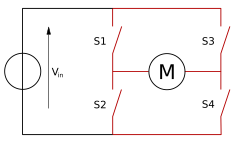
\includegraphics[width=0.5\linewidth]{Images/PuenteH/H_bridge.svg.png}
    \caption{Puente H Genérico por medio de llaves mecánicas}
\end{figure}

En este ejemplo, cuando la llave S1 y S4 se cierran, correrá corriente por esta rama, haciendo que el motor funcione y tenga un sentido de giro. Cuando la llave S2 y S3 se cierran, correrá corriente por esta rama también, pero con sentido de giro invertido. En este circuito, S1 y S2 nunca pueden estar cerradas al mismo tiempo, porque esto generaría un corto circuito, lo mismo con las llaves S3 y S4.

\begin{figure}[H]
    \centering
    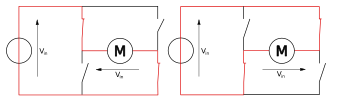
\includegraphics[width=0.70\linewidth]{Images/PuenteH/H_bridge_operating.svg.png}
    \caption{Puente H Operando}
\end{figure}

\subsubsection{Puente H de potencia}
Un puente H de potencia es un tipo de circuito en el que la etapa de potencia, que incluye el motor, los transistores y está conectada a altas tensiones y corrientes, se encuentra separada de la etapa de control, la cual generalmente opera con voltajes más bajos. Esta separación se realiza para proteger la etapa de control de las altas tensiones, que podrían dañar o quemar sus circuitos. Podemos utilizar nuestro puente H como ejemplo para ilustrar este concepto:

\begin{figure}[H]
    \centering
    \includegraphics[width=0.8\linewidth]{Images//PuenteH/Puente-H.jpg}
    \caption{Nuestro Puente H}
    \label{fig:enter-label}
\end{figure}

En nuestro puente H, hemos separado las ramas del motor de las de control, ya que el motor opera con 24V DC y tiene una corriente eficaz de 3,5A. Para controlar el motor de manera eficiente, hemos optado por un diseño que incluye cuatro transistores MOSFET de potencia, los cuales pueden soportar picos de hasta 74A y 82A, garantizando que puedan manejar la corriente del motor de manera continua. Los MOSFET son IRF2805 (canal N) y IRF4905 (canal P). Además, los transistores son controlados mediante señales PWM, las cuales atraviesan un optoacoplador EL817 para minimizar el riesgo de que la corriente del motor regrese a la placa de control y cause daños. De ésta manera, podemos controlar el giro del motor de manera segura y regulada. 

La lógica de esta circuito se basa en que cuando un MOSFET canal P está saturado, el gate del MOSFET de canal N cruzado se activará. Cuando el MOSFET canal P no está saturado, el MOSFET cruzado canal N no se activará. El circuito cuenta con diodos Zener de 12 Volts para regular la tensión de Gate-Source en cada uno de los transistores, ya que el límite es de 20 Volts.


\subsection{Sistema de recepción de señales por UART}
El sistema de recepción de señales implementado en este proyecto se fundamenta en la transmisión de datos en formato JSON, el cual es enviado desde el microcontrolador RP2040 Zero hacia la Raspberry Pi 4, utilizando el protocolo de comunicación UART (Universal Asynchronous Receiver-Transmitter). Este esquema de transmisión de datos asíncrono es clave para garantizar la correcta transferencia de la información entre ambos dispositivos, especialmente en sistemas donde la baja latencia y la alta velocidad son factores cruciales.

Cuando la RP2040 Zero actúa como transmisor y envía datos a través del enlace UART, se introduce un optoacoplador de alta velocidad, el modelo 6N137. Este componente tiene como función principal aislar eléctricamente las dos partes del circuito, asegurando que las señales y alimentaciones de los dispositivos conectados permanezcan separadas. Esto no solo mejora la seguridad del sistema, sino que también protege los componentes sensibles de posibles interferencias o fluctuaciones de voltaje que podrían ocasionar fallas operativas o daños permanentes. El uso de optoacopladores es una práctica común en la ingeniería de control y automatización para proteger circuitos en entornos electromagnéticamente ruidosos.

Posteriormente, la señal transmitida es procesada mediante un transistor BJT (Bipolar Junction Transistor) del modelo 2N2222, que invierte la lógica de la señal. Esta operación es fundamental para garantizar que la interpretación de los datos sea precisa en el extremo receptor, adaptando la señal a los requerimientos lógicos de la Raspberry Pi 4.

Es importante destacar la elección de estos componentes electrónicos, especialmente por la alta tasa de transmisión que maneja el sistema UART, la cual opera a una velocidad de 115200 baudios. Esta velocidad de transmisión es adecuada para aplicaciones de tiempo real, donde se requiere una comunicación rápida y eficiente, sin comprometer la integridad de los datos transmitidos. El uso de componentes rápidos y confiables, como el optoacoplador 6N137 y el transistor 2N2222, asegura que el sistema pueda operar de manera estable y eficiente bajo estas condiciones.

\subsection{Control por PWM}
La modulación por ancho de pulso (PWM, por sus siglas en inglés Pulse Width Modulation) es una técnica empleada para regular la cantidad de energía suministrada a una carga, como un motor o un LED, mediante la variación del ciclo de trabajo de una señal pulsante. En lugar de modificar el voltaje de forma continua, PWM ajusta el tiempo durante el cual la señal permanece en estado alto (encendida) y bajo (apagada) dentro de un período fijo. Esto depende de los siguientes parámetros:

\begin{itemize}
    \item \textbf{Frecuencia:} Se refiere a la cantidad de ciclos de encendido y apagado que ocurren en un segundo, y se mide en Hertz (Hz).
    \item \textbf{Ciclo de trabajo:} Es el porcentaje de tiempo que la señal se mantiene en estado alto durante un ciclo. Por ejemplo:
    Un ciclo de trabajo del 0\% implica que la señal está siempre apagada.
    Un ciclo de trabajo del 50\% significa que la señal está encendida la mitad del tiempo y apagada la otra mitad.
    Un ciclo de trabajo del 100\% indica que la señal permanece siempre encendida.
    En nuestro proyecto, aplicamos la técnica de PWM en el control de los motores. Dado que utilizamos dos motores, si estos operaran a su máxima potencia, la silla de ruedas se desplazaría a una velocidad excesiva. Por esta razón, empleamos un ciclo de trabajo del 25\% para limitar la velocidad de avance.
\end{itemize}

\begin{figure}[H]
    \centering
    \includegraphics[width=0.7\linewidth]{Images//PWM/PWM.png}
    \caption{Ejemplo de señal PWM}
    \label{fig:enter-label}
\end{figure}

\subsection{Estructura de la silla}
La estructura de la silla de ruedas está compuesta por varios elementos fundamentales que aseguran su funcionamiento eficiente y seguro. En primer lugar, se encuentra un soporte robusto, cuyo propósito principal es sostener y estabilizar los motores que impulsan la silla. Este soporte ha sido diseñado para garantizar que los motores permanezcan firmemente sujetos, evitando vibraciones o movimientos indeseados que pudieran comprometer la precisión y fiabilidad del sistema.

El sistema de propulsión de la silla está constituido por dos motores de corriente continua (CC), cada uno operando a 24 voltios. Estos motores ofrecen una potencia promedio de 200W y alcanzan una potencia máxima de 500W. Este rango de potencia permite que la silla se desplace con suficiente fuerza para adaptarse a diversas condiciones de uso, ya sea en terrenos planos o en situaciones que requieran mayor esfuerzo.

En cuanto al asiento de la silla, ha sido confeccionado específicamente para este proyecto, integrando un diseño ergonómico que prioriza la comodidad del usuario sin sacrificar la funcionalidad. En la parte posterior del respaldo de la silla se encuentra una caja diseñada para actuar como una "Jaula de Faraday". Esta caja tiene la función de aislar eléctricamente los componentes electrónicos ubicados en su interior, protegiéndolos de interferencias electromagnéticas externas. 

\section{Desarrollo Técnico}
En este capítulo se proporcionará una descripción detallada sobre el funcionamiento de los distintos circuitos que conforman el dispositivo, así como su interacción en conjunto para cumplir con los objetivos del proyecto. Se explicará de manera clara y concisa cómo se utiliza el dispositivo, incluyendo instrucciones específicas para su correcto manejo y operatividad.

Además, se incluirán datos técnicos relevantes, tales como especificaciones de los componentes, características del diseño, y cualquier otro detalle que sea esencial para la comprensión del sistema. También se abordarán aspectos importantes acerca de las partes constitutivas del dispositivo, su función dentro del esquema general, y las consideraciones necesarias para su mantenimiento y optimización.

\subsection{Descripción del funcionamiento}
El usuario se sienta en la silla de ruedas y se coloca el dispositivo EEG. El EEG capta las señales cerebrales (alfa, beta, gamma, delta y theta) y las somete a un proceso de filtrado por hardware que incluye un filtro notch de 50 Hz, un filtro pasa-bajo de 100 Hz, un filtro pasa-alto de 0,5 Hz y un segundo filtro notch de 50 Hz. Posteriormente, las señales pasan por un circuito de compensación de offset para poder realizar la lectura por parte de la RP2040 Zero ya que la misma no puede leer valores negativos. Esta unidad se encarga de leer los datos mediante cuatro canales de ADC y enviarlos a la Raspberry Pi 4 por protocolo UART, donde se aloja el programa principal para el funcionamiento de la silla de ruedas.

Entre estos códigos se encuentran el control de motores, los filtros digitales, el procesamiento de señales y la inteligencia artificial (IA). Una vez las señales llegan a la Raspberry Pi 4, se filtran digitalmente para eliminar el ruido y mejorar la calidad de los datos. Tras el filtrado, las señales se envían a la IA, que tiene la función de reconocer los patrones cerebrales y determinar la dirección en la que el usuario desea moverse. Una vez el patrón ha sido identificado, se envía una señal a los motores para dirigir la silla hacia la dirección deseada (adelante, atrás, izquierda o derecha).

Además, el proyecto incluye un sistema de emergencia diseñado para garantizar la seguridad del usuario. Este sistema se activa si se detecta un error en la lectura de las señales o si hay un obstáculo en la trayectoria deseada. Su objetivo es prevenir accidentes y aumentar la seguridad del usuario al utilizar la silla de ruedas.

El sistema de emergencia utiliza sensores de ultrasonido para detectar la presencia de objetos a menos de 20 cm de la silla. En caso de detección, el sistema frena los motores y activa un LED en la dirección del objeto, además de un buzzer que emite una señal sonora durante un breve período para alertar al usuario sobre la activación del sistema.

\subsection{Funcionamiento del EEG}

El sistema de control de nuestra silla de ruedas se basa en el reconocimiento de señales cerebrales, lo que requiere un dispositivo especializado para captarlas: el electroencefalograma (EEG). Hemos desarrollado un EEG en forma de una cofia equipada con electrodos, los cuales se colocan siguiendo el protocolo conocido como “Sistema 10-20”. Este sistema estándar de ubicación define puntos específicos en el cuero cabelludo donde se deben colocar los electrodos para obtener lecturas óptimas de la actividad cerebral.

Los electrodos actúan como sensores pasivos que detectan las ondas cerebrales producidas por la actividad eléctrica del cerebro. Estas ondas se manifiestan como pequeñas fluctuaciones en el voltaje, que son captadas por los electrodos cuando se colocan sobre la superficie del cuero cabelludo del usuario. Es importante destacar que estos electrodos no penetran en el cráneo ni interactúan directamente con las neuronas. En cambio, registran los potenciales eléctricos generados por la actividad cerebral subyacente que se propagan hasta la superficie del cuero cabelludo.

Debido a que las señales captadas por los electrodos son de muy baja amplitud, requieren ser amplificadas antes de su procesamiento. Este paso no solo amplifica la señal cerebral, sino también el ruido presente en el entorno o generado por el propio cuerpo. Para abordar este problema, se realiza un proceso de filtrado que elimina el ruido y permite aislar las frecuencias relevantes de las ondas cerebrales. Para ello, utilizamos los AD620AN que son amplificadores de instrumento muy sensibles.

Las frecuencias de las ondas cerebrales detectadas son las siguientes:

\begin{itemize}
    \item Ondas alfa: 8-12 Hz
    \item Ondas beta: 12-30 Hz
    \item Ondas gamma: 30-100 Hz
    \item Ondas delta: 0,5-4 Hz
    \item Ondas theta: 4-8 Hz
\end{itemize}

Estas ondas cerebrales están asociadas con diferentes estados mentales y actividades cerebrales, por ejemplo, las ondas alfa se observan comúnmente en estados de relajación, mientras que las ondas beta se relacionan con un estado de alerta y concentración. Las ondas gamma, por otro lado, están vinculadas a procesos cognitivos de mayor complejidad, como la percepción y la conciencia. Las ondas delta y theta se asocian con fases profundas del sueño y la meditación.

\subsection{Funcionamiento de los filtros HardWare}

En un sistema de EEG, después de amplificar las señales captadas por los electrodos, se utilizan varios filtros para limpiar y mejorar la calidad de las señales antes de procesarlas o analizarlas. Estos filtros tienen un propósito importante: eliminar el ruido y enfocarse en las señales cerebrales relevantes. 

\subsubsection{Filtro Notch de 50 Hz}
\begin{itemize}
    \item \textbf{Propósito:} Atenuación del ruido inducido por la red eléctrica de 50 Hz, común en muchos sistemas de distribución de energía.
    \item \textbf{Funcionamiento:} El filtro Notch es un filtro de rechazo de banda estrecha, diseñado para eliminar una frecuencia específica (en este caso, 50 Hz) sin afectar significativamente las componentes de frecuencia cercanas o las señales EEG de interés. Las señales de EEG, que suelen estar en el rango de 0,5 a 40 Hz, pueden contaminarse por la interferencia de la red, por lo que este filtro resulta esencial para su eliminación sin alterar la información relevante.
\end{itemize}
\subsubsection{Filtro pasa bajos de 100 Hz}
\begin{itemize}
    \item \textbf{Propósito:} Reducción de las componentes de alta frecuencia que no son relevantes para el análisis EEG.
    \item \textbf{Funcionamiento:} Este filtro pasa bajos permite el paso de frecuencias inferiores a 100 Hz, atenuando aquellas que exceden este umbral. Las señales cerebrales de interés generalmente se sitúan por debajo de los 40 Hz, aunque algunas pueden extenderse hasta 100 Hz. Este filtro elimina frecuencias más altas, que usualmente corresponden a interferencias electromagnéticas, ruido de dispositivos electrónicos o artefactos musculares (EMG).
\end{itemize}
\subsubsection{Filtro pasa altos de 0,5 Hz}
\begin{itemize}
    \item \textbf{Propósito:} Eliminación de las componentes de muy baja frecuencia, incluyendo artefactos de corriente continua (DC) y ruido de baja frecuencia no relacionado con la actividad cerebral.
    \item \textbf{Funcionamiento:} El filtro pasa altos atenúa las señales con frecuencias por debajo de 0,5 Hz, permitiendo únicamente el paso de frecuencias superiores. La señal EEG relevante generalmente comienza en torno a los 0,5 Hz, mientras que frecuencias menores suelen estar asociadas a artefactos como el desplazamiento de los electrodos, fluctuaciones en la impedancia de los mismos, o interferencias lentas que no contienen información útil sobre la actividad cerebral.
\end{itemize}

\subsection{Funcionamiento de los filtros digitales}

Una vez que las ondas cerebrales son captadas y sometidas a un proceso inicial de filtrado, son transferidas a una Raspberry Pi 4. En este dispositivo se ejecuta un programa, desarrollado íntegramente por nuestro equipo, que continúa con el procesamiento y refinamiento de la señal. El motivo por el cual se aplica un filtrado adicional es que, luego de la etapa de filtrado inicial, la señal pasa por un segundo amplificador. Este amplificador, además de amplificar las señales cerebrales de interés, también amplifica el ruido residual presente en las mismas. Para contrarrestar este efecto, empleamos filtros digitales implementados por software, los cuales ofrecen una mayor precisión y control en la eliminación de interferencias no deseadas.

Dentro del programa, se han implementado los siguientes filtros:
\begin{itemize}
    \item \textbf{Filtro Notch de 50 Hz:} Este filtro está diseñado para eliminar las interferencias generadas por la red eléctrica, las cuales operan a una frecuencia de 50 Hz. Dado que estas interferencias pueden superponerse con la señal cerebral y distorsionar su interpretación, su eliminación es esencial para obtener un registro más fiel de la actividad cerebral.
    \item \textbf{Filtro Pasa-Bajo de 100 Hz:} El objetivo de este filtro es retener las frecuencias cerebrales más relevantes, es decir, aquellas que se encuentran por debajo de los 100 Hz, mientras que elimina el ruido de alta frecuencia, que suele ser resultado de interferencias externas o artefactos no relacionados con la actividad cerebral. Este rango incluye frecuencias relacionadas con ritmos cerebrales importantes como las ondas alfa, beta, y gamma.
    \item \textbf{Filtro Pasa-Alto de 0,5 Hz:} Este filtro se encarga de remover las señales de baja frecuencia que no aportan información útil sobre la actividad cerebral, como los artefactos causados por movimientos lentos o variaciones de corriente. Solo se permite el paso de las frecuencias EEG relevantes, garantizando que las señales reflejen con mayor precisión la actividad neural de interés.
\end{itemize}

Es importante señalar que el uso de estos filtros garantiza que la señal procesada esté lo más limpia posible de interferencias y artefactos, mejorando la precisión del sistema para detectar y procesar patrones cerebrales. La implementación de filtros mediante software, además, permite ajustar dinámicamente las configuraciones según las necesidades específicas del sistema y del entorno operativo, optimizando así el rendimiento de la silla de ruedas controlada por señales cerebrales.

\subsection{Funcionamiento del Puente H}

El circuito utiliza dos señales PWM (PWM1 y PWM2) para controlar los transistores MOSFET en configuración de puente H, lo que permite invertir la polaridad del voltaje aplicado al motor, controlando así la dirección de rotación. 

La velocidad del motor puede controlarse ajustando el ciclo de trabajo (duty cycle) de las señales PWM, que modulan la cantidad de energía entregada al motor.

Este circuito es ideal para aplicaciones donde se requiere un control preciso de dirección y velocidad de motores DC.

\subsubsection{Descripción de los Componentes}

\begin{enumerate}

    \item \textbf{U1 y U2 (PC817 - Optoacopladores):} Aíslan eléctricamente el circuito de control (de baja tensión) del circuito de potencia (de alta tensión). Esto protege al microcontrolador de posibles picos de voltaje y ruidos eléctricos provenientes del circuito de potencia.
    Cada optoacoplador tiene un LED interno que, al ser activado por una señal PWM, enciende un fototransistor interno, permitiendo que la señal de control pase al lado de potencia.
    
    \item \textbf{Q1 y Q3 (IRF4905 - MOSFET canal P):} Actúan como interruptores en la parte superior del puente H. Controlan la alimentación positiva hacia el motor. Estos MOSFET se activan cuando la señal PWM1 o PWM2 está en bajo (0V) y se desactivan cuando está en alto (señal de 5V), debido a la naturaleza de los MOSFET de canal P.
    
    \item \textbf{Q2 y Q4 (IRF2805 - MOSFET canal N):} Actúan como interruptores en la parte inferior del puente H. Conectan el motor a tierra cuando están activados. Estos MOSFET se activan cuando la señal PWM1 o PWM2 está en alto (5V) y se desactivan cuando está en bajo (0V).
    
    \item \textbf{R1 y R2 (Resistencias de 180 ohms):} Limitan la corriente de entrada hacia los LEDs internos de los optoacopladores (U1 y U2) para protegerlos de daños.
    
    \item \textbf{R3 y R4 (Resistencias de 1k ohms):} Están conectadas en serie con los MOSFET de canal P (Q1 y Q3). Limitan la corriente de la compuerta y aseguran un apagado rápido del MOSFET al detenerse la señal.
    
    \item \textbf{J1 y J2 (Conectores de entrada PWM):} Reciben las señales PWM de control provenientes de un microcontrolador o una fuente de señal PWM.
    
    \item \textbf{J3 y J4 (Conectores de alimentación):} Proveen la alimentación al circuito, uno con 24V para el motor y otro con 15V para los circuitos de control.
    
    \item \textbf{SW1 (Interruptor):}  utilizado para habilitar o deshabilitar el circuito completo, conectando o desconectando GND.
    
\end{enumerate}


\subsection{Funcionamiento del Sistema de Emergencia}
El sistema de emergencia de nuestra silla de ruedas controlada mediante señales cerebrales es un componente crítico para la seguridad del usuario, diseñado específicamente para evitar colisiones y accidentes en caso de que el usuario intente desplazarse hacia una dirección donde exista un obstáculo. Este sistema está integrado con los sensores ultrasónicos, que actúan como "ojos" del sistema, escaneando constantemente el entorno alrededor de la silla en cuatro direcciones: adelante, atrás, izquierda y derecha.

El funcionamiento es sencillo:

\begin{enumerate}
    \item \textbf{Detección de Obstáculos:} Cada uno de los sensores ultrasónicos está ubicado estratégicamente en una de las direcciones mencionadas. Estos sensores emiten pulsos ultrasónicos que se reflejan al chocar con un objeto, lo que permite calcular la distancia al obstáculo con alta precisión. Si el sistema detecta un objeto en la dirección hacia la cual el usuario ha decidido moverse, el sensor ultrasónico correspondiente enviará una señal de alerta al sistema de control.
    \item \textbf{Intervención Automática:} Una vez que se detecta un obstáculo en la trayectoria, el sistema de emergencia interviene automáticamente para detener el movimiento de los motores. Esto se logra mediante la interrupción de las señales de control enviadas por la Raspberry Pi 4 a los motores, utilizando la modulación PWM. Al cortar las señales de control de los motores, se asegura que la silla no avance hacia la dirección donde se ha identificado el peligro.
    \item \textbf{Señales Visuales y Auditivas:} Al mismo tiempo que se detienen los motores, el sistema activa una señal auditiva mediante un buzzer, que emite un sonido de advertencia. Además, se enciende un LED específico que indica la dirección donde se encuentra el obstáculo, proporcionando una indicación visual clara tanto para el usuario como para quienes estén cerca. Estos elementos visuales y auditivos aseguran que la persona a cargo de la silla, o cualquier acompañante, esté consciente del riesgo potencial en la dirección de movimiento.
    \item \textbf{Restablecimiento del Movimiento:} Una vez que el obstáculo es removido, o el usuario decide cambiar la dirección de movimiento hacia un área despejada, el sistema de emergencia desactiva automáticamente las señales de advertencia (buzzer y LED), y el control de los motores se restablece, permitiendo que la silla continúe su desplazamiento normal. Este proceso es completamente autónomo, sin necesidad de intervención manual.
    \item \textbf{Integración con el Sistema de Control Principal:} El sistema de emergencia está completamente integrado con el sistema de control principal basado en la Raspberry Pi 4. Todos los sensores ultrasónicos, buzzer y LEDs están conectados a los GPIOs de la Raspberry Pi, permitiendo una comunicación eficiente entre los distintos componentes. Además, el sistema de emergencia está diseñado para operar en tiempo real, lo que garantiza una respuesta inmediata ante cualquier detección de peligro.
\end{enumerate}

\subsection{Explicacion de los codigos utlizados}
En este apartado se explicaran los codigos utilizados en el proyecto y porqué los hemos utilizados.

\subsubsection{Explicacion de bias.py}
Este codigo es la clase organizadora de las demas clases que contienen: recepcion, filtrado, IA y movimiento de motor.

En este codigo se crea la clase principal: BiasClass.
\begin{lstlisting}[language=Python]
    class BiasClass:
    def __init__(self, n, fs, channels, port, baudrate, timeout):
        # Define properties for the class
        self._n = n
        self._fs = fs
        self._number_of_channels = channels
        self._duration = self._n / self._fs
        self._port = port
        self._baudrate = baudrate
        self._timeout = timeout
        self._commands = ["forward", "backwards", "left", "right", "stop", "rest"]
        self._samples_trainig_command = 100
\end{lstlisting}
\begin{itemize}
    \item \textbf{Propiedades:} Se inicializan varias propiedades para manejar parámetros de la clase, como el número de muestras n, la frecuencia de muestreo fs, el número de canales EEG, y las configuraciones del puerto serie para la recepción de datos.
    \item \textbf{Comandos:} Se define una lista de comandos posibles que la IA debe predecir para controlar el movimiento de la silla de ruedas.
\end{itemize}

\begin{lstlisting}
    self._biasReception = ReceptionBias(self._port, self._baudrate, self._timeout)
self._biasFilter = FilterBias(n=self._n, fs=self._fs, notch=True, bandpass=True, fir=False, iir=False)
self._biasProcessing = ProcessingBias(n=self._n, fs=self._fs)
self._biasGraphing = GraphingBias(graph_in_terminal=True)
self._biasMotor = MotorBias(...)
self._biasAI = AIBias(self._n, self._fs, self._number_of_channels, self._commands)
\end{lstlisting}
Aquí se crean objetos de distintas clases que se utilizarán en los métodos de la clase:
\begin{itemize}
    \item \textbf{ReceptionBias:} Para recibir datos desde los electrodos EEG.
    \item \textbf{FilterBias:} Para aplicar filtros digitales (notch, bandpass).
    \item \textbf{ProcessingBias:} Para procesar las señales EEG.
    \item \textbf{GraphingBias:} Para graficar las señales en tiempo real.
    \item \textbf{MotorBias:} Para controlar los motores en respuesta a los comandos predichos por la IA.
    \item \textbf{AIBias:} Para entrenar el modelo de IA y predecir comandos basados en los datos EEG.
\end{itemize}

\begin{lstlisting}
    def train_ai_model(self, save_path, saved_dataset_path):
    self._biasAI.collect_and_train(reception_instance=self._biasReception, filter_instance=self._biasFilter,
                                   processing_instance=self._biasProcessing, 
                                   samples_per_command=self._samples_trainig_command, save_path=save_path,
                                   saved_dataset_path=saved_dataset_path, real_data=True)

\end{lstlisting}

Este método permite entrenar un modelo de IA con datos de señales EEG en tiempo real:
\begin{itemize}
    \item \textbf{collect\_and\_train:} Este método recolecta datos, los filtra, procesa y luego entrena la IA para reconocer comandos a partir de señales EEG.
    \item \textbf{Parámetros:} save\_path y saved\_dataset\_path indican los caminos donde se guardan los datos entrenados o el conjunto de datos usado.
\end{itemize}

\begin{lstlisting}
    def app_run(self):
    while True:
        # Receive eeg data
        signals = self._biasReception.get_real_data(channels=self._number_of_channels, n=self._n)
        
        # Graph signals
        for ch, signal in signals.items():
            t = np.arange(len(signals[ch])) / self._fs
            self._biasGraphing.graph_signal_voltage_time(t=t, signal=np.array(signal), title="Signal {}".format(ch))
        
        # Apply digital filtering
        filtered_data = self._biasFilter.filter_signals(signals)
        
        # Graph filtered signals
        t = np.linspace(0, self._duration, self._n, endpoint=False)
        for ch, signal in filtered_data.items():
            self._biasGraphing.graph_signal_voltage_time(t=t, signal=signal, title="Filtered Signal {}".format(ch))
        
        # Process data
        times, eeg_signals = self._biasProcessing.process_signals(filtered_data)
        
        # Graph processed EEG signals by band
        for ch, signals in eeg_signals.items():
            for band_name, sig in signals.items():
                self._biasGraphing.graph_signal_voltage_time(t=times[ch], signal=sig, title=f"{band_name.capitalize()} interpolated. {ch}")
        
        # Plot now
        self._biasGraphing.plot_now()

        # Predict and move motors
        #command = self._biasAI.predict_command(eeg_data=eeg_signals)
        #self._biasMotor.move_if_possible(command)
\end{lstlisting}
\begin{itemize}
    \item \textbf{Recepción de datos EEG:} Se utiliza get\_real\_data para obtener señales EEG en tiempo real.
    \item \textbf{Graficación de señales sin filtrar:} Se grafican las señales sin filtrar usando GraphingBias.
    \item \textbf{Filtrado digital:} Se aplican filtros a las señales mediante FilterBias.
    \item \textbf{Procesamiento:} Las señales filtradas son procesadas usando ProcessingBias.
    \item \textbf{Predicción de comandos (comentada):} El código está preparado para usar IA para predecir un comando basado en las señales EEG procesadas, pero esta parte está comentada.
    \item \textbf{Control de motores:} Según el comando predicho, se puede mover la silla de ruedas.
\end{itemize}

\subsubsection{Explicacion bias\_ai.py}
En este codigo se programa la IA. Es donde la IA esta la IA y se entrena con datasets.

\begin{lstlisting}
    def main():
    n = 1000
    fs = 500
    online = True
    number_of_channels = 4
    port = '/dev/serial0'
    baudrate = 115200
    timeout = 1
    biasReception = ReceptionBias(port, baudrate, timeout)
    biasFilter = FilterBias(n=n, fs=fs, notch=True, bandpass=True, fir=False, iir=False)
    biasProcessing = ProcessingBias(n=n, fs=fs)
    commands = ["forward", "backwards", "left", "right", "stop", "rest"]
    biasAI = AIBias(n=n, fs=fs, channels=number_of_channels, commands=commands)
    train = input("Do you want to train model? (y/n): ")
    if train.lower() == "y":
        saved_dataset_path = None
        save_path = None
        loading_dataset = input("Do you want to load a existent dataset? (y/n): ")
        if loading_dataset.lower() == "y":
            saved_dataset_path = input("Write the name of the file where dataset was saved: ")
        else:
            save_new_dataset = input("Do you want to save the new dataset? (y/n): ")
            if save_new_dataset == "y":
                save_path = input("Write the path where you want to save the dataset: ")
        biasAI.collect_and_train(reception_instance=biasReception, filter_instance=biasFilter, processing_instance=biasProcessing, 
                                 trials_per_command=1, save_path=save_path, saved_dataset_path=saved_dataset_path, real_data=False)
    # Generate synthetic data
    signals = generate_synthetic_eeg(n_samples=n, n_channels=number_of_channels, fs=fs, command="left")
    #signals = biasReception.get_real_data(channels=number_of_channels, n=n)
    
    filtered_data = biasFilter.filter_signals(signals)
    # Process data
    times, eeg_signals = biasProcessing.process_signals(filtered_data)
    predicted_command = biasAI.predict_command(eeg_data=eeg_signals)
    print(f"Predicted Command: {predicted_command}")
\end{lstlisting}
La función main() es el punto de entrada del programa y orquesta la inicialización y ejecución del sistema.

\textbf{Flujo de la Función Principal:}
\begin{enumerate}
    \item \textbf{Configuración Inicial:} Define parámetros esenciales como el número de muestras, frecuencia de muestreo, número de canales, puerto serial y velocidad de comunicación.
    \item \textbf{Inicialización de Objetos:}
    \begin{itemize}
        \item \textbf{ReceptionBias:} Maneja la recepción de datos EEG desde el puerto serial.
        \item \textbf{FilterBias:} Aplica filtros Notch y Bandpass para limpiar las señales EEG.
        \item \textbf{ProcessingBias:} Procesa las señales filtradas para extraer información relevante.
        \item \textbf{AIBias:} Gestiona la IA encargada de interpretar las señales y predecir comandos.
    \end{itemize}
    \item \textbf{Entrenamiento del Modelo de IA:} Ofrece al usuario la opción de entrenar el modelo, ya sea cargando un dataset existente o creando uno nuevo con datos reales o sintéticos.
    \item \textbf{Generación de Datos Sintéticos:} Crea señales EEG simuladas para pruebas sin necesidad de hardware físico.
    \item \textbf{Filtrado y Procesamiento de Señales:} Limpia y prepara las señales para la extracción de características.
    \item \textbf{Predicción de Comandos:} Utiliza el modelo entrenado para interpretar las señales EEG y determinar el comando de movimiento correspondiente.
\end{enumerate}

La clase AIBias es responsable de manejar todo el ciclo de vida del modelo de IA, desde la recopilación de datos hasta la predicción de comandos basados en las señales EEG.

\begin{lstlisting}
    class AIBias:
    def __init__(self, n, fs, channels, commands):
        # Inicialización de parámetros y estructuras de datos
        self._n = n
        self._fs = fs
        self._number_of_channels = channels
        self._features_length = len(["mean", "variance", "skewness", "kurt", "energy",
                                 "band_power", "wavelet_energy", "entropy"])
        self._number_of_waves_per_channel = len(["alpha", "beta", "gamma", "delta", "theta"])
        self._num_features_per_channel = self._features_length * self._number_of_waves_per_channel
        self._commands = commands
        self._model = self.build_model(output_dimension=len(self._commands))
        self._is_trained = False
        self._pca = PCA(n_components=0.95)  # Retiene el 95% de la varianza
        self._scaler = StandardScaler()

        # Mapeo dinámico de etiquetas basado en los comandos proporcionados
        self._label_map = {command: idx for idx, command in enumerate(self._commands)}
        self._reverse_label_map = {idx: command for command, idx in self._label_map.items()}

    # Getter para verificar si el modelo ha sido entrenado
    def ai_is_trained(self):
        return self._is_trained

    def collect_and_train(self, reception_instance, filter_instance, processing_instance, trials_per_command, 
                          save_path=None, saved_dataset_path=None, real_data=True):
        """
        Recopila datos EEG, extrae características y entrena el modelo.
        """
        X = []
        y = []

        if saved_dataset_path is None:
            for trial in range(trials_per_command):
                for command in self._commands:
                    # Obtener datos reales o generar datos sintéticos
                    if real_data:
                        print(f"Think about {command}. Trial: {trial}")
                        signals = reception_instance.get_real_data(channels=self._number_of_channels, n=self._n)
                    else:
                        print(f"Trial: {trial}")
                        signals = generate_synthetic_eeg(n_samples=self._n, n_channels=self._number_of_channels, fs=self._fs, command=command)
                    
                    # Filtrar y procesar las señales
                    filtered_data = filter_instance.filter_signals(signals)
                    _, eeg_signals = processing_instance.process_signals(filtered_data)

                    # Extraer características y añadir a X
                    features = self.extract_features(eeg_signals)
                    
                    X.append(features)
                    y.append(self._label_map[command])

                    if real_data:
                        time.sleep(1)
                
                if real_data:
                    print("Changing command. Be ready")
                    time.sleep(20)

            # Convertir X y y a arrays de Numpy
            X = np.array(X)
            y = np.array(y)

            if save_path:
                # Guardar el dataset como un archivo comprimido de Numpy
                np.savez_compressed(f"{save_path}.npz", X=X, y=y)
                print(f"Dataset saved to {save_path}.npz")
        
        else:
            # Cargar dataset existente
            data = np.load(f"{saved_dataset_path}.npz")
            X, y = data['X'], data['y']

        # Convertir y a codificación one-hot
        lb = LabelBinarizer()
        y = lb.fit_transform(y)

        # Entrenar el modelo con los datos recopilados
        self.train_model(X, y)

    def build_model(self, output_dimension):
        """
        Construye y compila el modelo de red neuronal.
        """
        model = Sequential([
            InputLayer(shape=(self._number_of_channels, self._num_features_per_channel)),
            Conv1D(filters=64, kernel_size=3, activation='relu'),
            MaxPooling1D(pool_size=1),
            Dropout(0.5),
            Flatten(),
            Dense(100, activation='relu'),
            Dropout(0.5),
            Dense(50, activation='relu'),
            Dropout(0.5),
            Dense(output_dimension, activation='softmax')  # 6 clases de salida
        ])
        model.compile(optimizer='adam', loss='categorical_crossentropy', metrics=['accuracy'])
        return model

    def extract_features(self, eeg_data):
        """
        Extrae características estadísticas y en el dominio de la frecuencia de las señales EEG.
        """
        features = []
        # Iterar sobre cada canal en eeg_data
        for ch, signals_per_channel in eeg_data.items():
            channel_features = []
            assert(len(signals_per_channel) == self._number_of_waves_per_channel)
            # Iterar sobre las señales de cada canal
            for band_name, signal_wave in signals_per_channel.items():
                signal_wave = np.array(signal_wave)

                # Características estadísticas
                mean = np.mean(signal_wave)
                variance = np.var(signal_wave)
                skewness = skew(signal_wave)
                kurt = kurtosis(signal_wave)
                energy = np.sum(signal_wave ** 2)

                # Características en el dominio de la frecuencia (Densidad Espectral de Potencia)
                freqs, psd = welch(signal_wave, fs=self._fs)  # fs = 500 Hz

                # Potencia de banda
                band_power = np.sum(psd)  # Potencia total dentro de esta banda

                # Energía de wavelet utilizando CWT con la función morlet
                scales = np.arange(1, 31)
                coeffs = cwt(signal_wave, morlet, scales)
                wavelet_energy = np.sum(coeffs ** 2)

                # Entropía
                signal_entropy = entropy(np.histogram(signal_wave, bins=10)[0])

                list_of_features = [mean, variance, skewness, kurt, energy, band_power, wavelet_energy, signal_entropy]

                # Añadir todas las características juntas
                channel_features.extend(list_of_features)
                
                assert(len(list_of_features) == self._features_length)
                
            features.append(channel_features)

        features = np.abs(np.array(features))
        features = self._scaler.fit_transform(features)  # Normalización
        # features = self._pca.fit_transform(features)  # Reducción de dimensionalidad (actualmente comentada)

        # Ajustar la forma basada en el tamaño real
        num_features_per_channel = features.shape[1]
        assert(self._num_features_per_channel == num_features_per_channel)
        expected_shape = (self._number_of_channels, self._num_features_per_channel)
        features = features.reshape(expected_shape)
        return features

    def train_model(self, X, y):
        """
        Entrena el modelo de red neuronal con los datos proporcionados.
        """
        X_train, X_test, y_train, y_test = train_test_split(X, y, test_size=0.2, random_state=42)
        self._model.fit(X_train, y_train, epochs=10, batch_size=32, validation_data=(X_test, y_test))
        self._is_trained = True

    def predict_command(self, eeg_data):
        """
        Predice el comando de movimiento basado en las señales EEG proporcionadas.
        """
        if not self._is_trained:
            raise Exception("Model has not been trained yet.")
        
        # Extraer características de los datos EEG
        features = self.extract_features(eeg_data)
        
        # Asegurar que las características tienen la forma correcta
        features = features.reshape(1, self._number_of_channels, self._num_features_per_channel)
        
        # Realizar la predicción
        prediction = self._model.predict(features)
        
        # Obtener el índice de la etiqueta predicha
        predicted_label_index = np.argmax(prediction, axis=1)[0]
        
        # Convertir el índice numérico a la etiqueta de texto correspondiente
        predicted_command = self._reverse_label_map[predicted_label_index]
        
        return predicted_command
\end{lstlisting}
\textbf{Funciones Clave de la Clase AIBias:}

\begin{enumerate}
    \item Constructor (\_\_init\_\_):
    \begin{itemize}
        \item Parámetros Iniciales:
        \begin{itemize}
            \item n: Número de muestras por canal.
            \item fs: Frecuencia de muestreo.
            \item channels: Número de canales EEG.
            \item commands: Lista de comandos que el modelo debe reconocer.
        \end{itemize}
        \item Configuración de features:
        \begin{itemize}
            \item Define la longitud de las características extraídas por banda de frecuencia.
            \item Calcula el número total de características por canal.
        \end{itemize}
        \item Modelo de IA: Construye y compila un modelo de red neuronal utilizando la función build\_model.
        \item Preprocesamiento: Inicializa escaladores (StandardScaler) y reducción de dimensionalidad (PCA).
        \item Mapeo de Etiquetas: Crea mapas para convertir comandos en índices numéricos y viceversa.
    \end{itemize}
    \item Método collect\_and\_train:
    \begin{itemize}
        \item Propósito: Recopila datos EEG (reales o sintéticos), extrae características y entrena el modelo de IA.
        \item Proceso:
        \begin{itemize}
            \item Si no se proporciona una ruta de dataset existente, recopila datos para cada comando, filtra y procesa las señales, extrae características y las almacena en X y y.
            \item Opcionalmente guarda el dataset recopilado.
            \item Si se proporciona una ruta de dataset existente, carga los datos directamente.
            \item Convierte las etiquetas y a una codificación one-hot para el entrenamiento.
           \item Llama al método train\_model para entrenar el modelo con los datos recopilados.
        \end{itemize}
    \end{itemize}
    \item Método build\_model:
    \begin{itemize}
        \item Descripción: Construye una red neuronal secuencial con las siguientes capas:
        \begin{itemize}
            \item InputLayer: Define la forma de entrada basada en el número de canales y características.
            \item Conv1D: Capa convolucional para detectar patrones en las señales.
            \item MaxPooling1D: Reducción de dimensionalidad.
            \item Dropout: Prevención de sobreajuste.
            \item Flatten: Aplana las salidas para las capas densas.
            \item Dense: Capas completamente conectadas para clasificación.
            \item Softmax: Capa de salida para clasificación multiclase.
        \end{itemize}
        \item Compilación del Modelo: Utiliza el optimizador 'adam', la función de pérdida 'categorical\_crossentropy' y métrica de precisión.
    \end{itemize}
    \item Método extract\_features:
    \begin{itemize}
        \item Propósito: Extrae Features estadísticas y de dominio de frecuencia de las señales EEG.
        \item Features Extraídas:
        \begin{itemize}
            \item Estadísticas: Media, varianza, asimetría, curtosis, energía.
            \item Frecuencia: Potencia espectral de banda, energía de wavelet.
            \item Entropía: Medida de la incertidumbre o aleatoriedad de la señal.
        \end{itemize}
        \item Proceso:
        \begin{itemize}
            \item Itera sobre cada canal y cada banda de frecuencia para calcular las Features.
            \item Normaliza las Features utilizando StandardScaler.
            \item Opcionalmente aplica PCA para reducir la dimensionalidad (actualmente comentado).
            \item Reorganiza las Features en la forma esperada para el modelo.
        \end{itemize}
    \end{itemize}
    \item Método train\_model:
    \begin{itemize}
        \item Descripción: Divide los datos en conjuntos de entrenamiento y prueba, entrena el modelo y actualiza el estado de entrenamiento.
        \item Proceso:
        \begin{itemize}
            \item Utiliza train\_test\_split para dividir los datos.
            \item Entrena el modelo con las características y etiquetas de entrenamiento.
            \item Valida el modelo con el conjunto de prueba.
            \item Marca el modelo como entrenado.
        \end{itemize}
    \end{itemize}
    \item Método predict\_command:
    \begin{itemize}
        \item Descripción: Predice el comando de movimiento basado en nuevas señales EEG.
        \newpage
        \item Proceso:
        \begin{itemize}
            \item Verifica si el modelo ha sido entrenado.
            \item Extrae características de las señales EEG proporcionadas.
            \item Ajusta la forma de las características para la predicción.
            \item Utiliza el modelo para predecir el comando.
            \item Convierte la predicción numérica a la etiqueta de comando correspondiente.
        \end{itemize}
    \end{itemize}
\end{enumerate}
\begin{lstlisting}
    def generate_synthetic_eeg(n_samples, n_channels, fs, command=None):
    """
    Genera datos EEG sintéticos para múltiples canales.
    La salida es un diccionario donde cada canal tiene 1000 muestras crudas.
    Simula diferentes tareas alterando los patrones de la señal.
    """
    t = np.linspace(0, n_samples/fs, n_samples, endpoint=False)
    data = {}

    for ch in range(n_channels):
        # Simular diferentes bandas de frecuencia con algunas correlaciones básicas
        base_alpha = np.sin(2 * np.pi * 10 * t)  # Alpha (10 Hz)
        base_beta = np.sin(2 * np.pi * 20 * t)   # Beta (20 Hz)
        base_theta = np.sin(2 * np.pi * 6 * t)   # Theta (6 Hz)
        base_delta = np.sin(2 * np.pi * 2 * t)   # Delta (2 Hz)
        base_gamma = np.sin(2 * np.pi * 40 * t)  # Gamma (40 Hz)

        alpha_power = 1.0
        beta_power = 1.0
        theta_power = 1.0
        delta_power = 1.0
        gamma_power = 1.0  # Ajustar señal según el comando

        if command == "forward":
            alpha_power = 1.5
            beta_power = 0.5
        elif command == "backward":
            alpha_power = 0.5
            beta_power = 1.5
        elif command == "left":
            theta_power = 1.5
            delta_power = 0.5
        elif command == "right":
            theta_power = 0.5
            delta_power = 1.5
        elif command == "stop":
            alpha_power = 0.2
            beta_power = 0.2
            gamma_power = 0.2
        else:  # rest
            alpha_power = 1.0
            beta_power = 1.0
            theta_power = 1.0
            delta_power = 1.0
            gamma_power = 1.0        

        # Generar señal con algo de aleatoriedad y correlaciones
        signal = (
            alpha_power * base_alpha +
            beta_power * base_beta +
            theta_power * base_theta +
            delta_power * base_delta +
            gamma_power * base_gamma
        )

        # Añadir correlación entre canales (e.g., 10% de la señal del canal anterior)
        if ch > 0:
            signal += 0.1 * data[ch-1]

        # Añadir ruido aleatorio para simular señales EEG realistas
        noise = np.random.normal(0, 0.1, size=t.shape)
        signal += noise

        # Almacenar la señal cruda en el diccionario
        data[ch] = signal

    return data
\end{lstlisting}
Características de la Función:
\begin{itemize}
    \item \textbf{Simulación de Bandas de Frecuencia:} Crea señales para diferentes bandas (Alpha, Beta, Theta, Delta, Gamma) ajustando sus amplitudes según el comando simulado.
    \item \textbf{Correlación entre Canales:} Introduce una correlación simple entre canales adyacentes para mayor realismo.
    \item \textbf{Ruido Aleatorio:} Añade ruido gaussiano para emular las imperfecciones de las señales EEG reales.
    \item \textbf{Flexibilidad de Comandos:} Permite ajustar las características de las señales según el comando que se está simulando (e.g., "forward", "left").
\end{itemize}

\subsubsection{Explicacion bias\_dsp.py}
Este código implementa un flujo completo de recepción, filtrado y procesamiento de señales EEG utilizando diversas técnicas de procesamiento digital de señales (DSP). A continuación, explicaré cada parte clave del código:

\begin{lstlisting}
    class DSPBias:
    def __init__(self, n, fs):
        self._n = n
        self._fs = fs
        self._duration = self._n / self._fs
\end{lstlisting}
Esta es una clase base que inicializa las propiedades comunes para las operaciones de DSP, como la cantidad de muestras (n), la frecuencia de muestreo (fs), y la duración de la señal. Es utilizada como punto de partida para clases que heredan estas características.

\begin{lstlisting}
    class ProcessingBias(DSPBias):
    def __init__(self, n, fs):
        super().__init__(n, fs)
        self._biasGraphing = GraphingBias(graph_in_terminal=False)
\end{lstlisting}
Esta clase hereda de DSPBias y añade la funcionalidad de procesamiento de señales EEG. En el método process\_signals, se procesa cada señal en los canales EEG y se grafican en el dominio del tiempo y frecuencia.

\begin{lstlisting}
    def do_fft(self, signal):
    signal_fft = np.fft.fft(signal)
    frequencies = np.fft.fftfreq(self._n, d=1/self._fs)
    signal_fft_magnitude = np.abs(signal_fft) / self._n
    return signal_fft, frequencies, signal_fft_magnitude
\end{lstlisting}
Este método realiza la Transformada de Fourier para convertir la señal del dominio del tiempo al dominio de la frecuencia, permitiendo analizar los componentes de frecuencia de la señal EEG.

\begin{lstlisting}
    class FilterBias(DSPBias):
    def __init__(self, n, fs, notch, bandpass, fir, iir):
        self._notch = notch
        self._bandpass = bandpass
        self._fir = fir
        self._iir = iir
        super().__init__(n=n, fs=fs)
\end{lstlisting}
Esta clase implementa varios tipos de filtros digitales, como:
\begin{itemize}
    \item \textbf{Notch Filter:} Para eliminar interferencias de frecuencia específicas (por ejemplo, ruido de la línea de energía a 50 Hz).
    \item \textbf{Bandpass Filter:} Para filtrar un rango de frecuencias.
    \item \textbf{FIR e IIR Filters:} Filtros de paso bajo que permiten suavizar las señales.
\end{itemize}

\begin{lstlisting}
    def butter_bandpass_filter(self, data, lowcut, highcut, order=5):
    nyquist = 0.5 * self._fs
    low = lowcut / nyquist
    high = highcut / nyquist
    b, a = butter(order, [low, high], btype='band')
    y = filtfilt(b, a, data, axis=1)
    return y
\end{lstlisting}
Este método aplica un filtro de paso de banda usando un filtro Butterworth. Este tipo de filtro permite el paso de un rango específico de frecuencias, bloqueando las demás.

Dentro de main, después de recibir las señales del hardware (ReceptionBias), las señales son graficadas antes y después del filtrado. Luego, las señales filtradas son procesadas usando Fourier y graficadas en diferentes bandas de EEG.

\begin{lstlisting}
    for ch, signal in filtered_data.items():
    biasGraphing.graph_signal_voltage_time(t=t, signal=signal, title="Filtered Signal {}".format(ch))
\end{lstlisting}
Aquí se grafican las señales filtradas para observar cómo se ven en el dominio del tiempo, permitiendo una inspección visual de los efectos del filtrado.
\begin{lstlisting}
    def interpolate_signal(self, t, signal, new_t):
    interpolated_signal = scipy.interpolate.interp1d(t, signal, kind='cubic')(new_t)
    return interpolated_signal
\end{lstlisting}
Este método interpola las señales para mejorar la resolución temporal, lo cual es útil cuando se desea obtener más puntos de datos entre las muestras originales.

\subsubsection{Explicacion bias\_graphing.py}
En este codigo se realiza los graficos de las señales en funcion del tiempo y la frecuencia. En el contexto de nuestro proyecto, la clase "GraphingBias" se utiliza para visualizar las señales cerebrales captadas por el sistema EEG de nuestra silla de ruedas. Estas señales se pueden representar tanto en el dominio del tiempo como en el de la frecuencia, lo que es crucial para entender la actividad cerebral y ajustar los patrones de control de la silla.

\begin{lstlisting}
    class GraphingBias:
    # Constructor
    def __init__(self, graph_in_terminal):
        self._graph_in_terminal = graph_in_terminal
\end{lstlisting}
El constructor inicializa la clase GraphingBias, recibiendo como parámetro graph\_in\_terminal, que es un valor booleano. Este parámetro determina si los gráficos se deben visualizar en la terminal (True) o en una ventana gráfica externa usando matplotlib (False).
\begin{lstlisting}
    def graph_signal_voltage_time(self, t, signal, title):
    if not self._graph_in_terminal:
        plt.figure(figsize=(12, 6))
        if signal.ndim == 1:
            plt.plot(t, signal)
        else:
            for i in range(signal.shape[0]):
                plt.plot(t, signal[i])
        plt.title(title)
        plt.xlabel("Time [s]")
        plt.ylabel("Magnitude")
        plt.grid()
    else:
        plotext.clear_data()
        plotext.plot(t, signal)
        plotext.title(title)
        plotext.xlabel("Time [s]")
        plotext.ylabel("Magnitude")
        plotext.show()
\end{lstlisting}
Esta función grafica la señal en el dominio del tiempo, donde el eje x representa el tiempo (en segundos) y el eje y representa la magnitud de la señal. Dependiendo de si se selecciona graficar en la terminal o en una interfaz gráfica, se utilizan diferentes librerías (matplotlib o plotext).
\begin{itemize}
    \item Si self.\_graph\_in\_terminal es False, se usa matplotlib para graficar en una ventana gráfica.
    \item Si es True, se usa plotext para graficar directamente en la terminal.
\end{itemize}

\begin{lstlisting}
    def graph_signal_voltage_frequency(self, frequencies, magnitudes, title):
    if not self._graph_in_terminal:
        plt.figure(figsize=(12, 6))
        plt.plot(frequencies, magnitudes)
        plt.title(title)
        plt.xlabel("Frequency [Hz]")
        plt.ylabel("Magnitude")
        plt.grid()
    else:
        plotext.clear_data()
        plotext.plot(frequencies, magnitudes)
        plotext.title(title)
        plotext.xlabel("Frequency [Hz]")
        plotext.ylabel("Magnitude")
        plotext.show()
\end{lstlisting}
Esta función grafica la señal en el dominio de la frecuencia. En el eje x, se representan las frecuencias (en Hz), y en el eje y, las magnitudes de la señal para cada frecuencia. Nuevamente, dependiendo del valor de self.\_graph\_in\_terminal, se selecciona si se grafica en una interfaz gráfica o directamente en la terminal.

\begin{lstlisting}
    def plot_now(self):
    if not self._graph_in_terminal:
        plt.tight_layout()
        plt.show()
    else:
        pass
\end{lstlisting}
Esta función se encarga de mostrar el gráfico después de haberlo configurado. Si estamos usando matplotlib, se asegura de que el diseño del gráfico sea el adecuado (tight\_layout) y luego lo muestra en pantalla. Si estamos graficando en la terminal, no hace nada, ya que la función plotext.show() ya gestiona la visualización.

\begin{lstlisting}
    if not self._graph_in_terminal:
    # Uso de matplotlib
else:
    # Uso de plotext
\end{lstlisting}
Estas estructuras determinan si los gráficos se crean usando matplotlib o plotext, dependiendo de si estamos trabajando en un entorno gráfico o en la terminal.

\subsubsection{Explicacion bias\_motors.py}
Este código controla el movimiento de la silla de ruedas utilizando un conjunto de sensores ultrasónicos, LEDs, un buzzer, y motores. Dependiendo del comando ingresado por el usuario (forward, left, backwards, right o stop), la silla de ruedas se mueve en la dirección indicada o se detiene. Los sensores ultrasónicos verifican si hay obstáculos a menos de 20 cm, y si se detecta uno, los LEDs y el buzzer se activan para alertar al usuario y bloquear el movimiento.

\begin{lstlisting}
    def main():
    biasMotor = MotorBias(echo_forward=18, trigger_forward=17, echo_backwards=23, trigger_backwards=22, 
                          echo_right=5, trigger_right=6, echo_left=25, trigger_left=24, 
                          led_forward=16, led_backwards=20, led_left=21, led_right=26, 
                          buzzer=12, motor1_in1=13, motor1_in2=19, motor2_in1=7, motor2_in2=8)
    while True:
        command = input("Enter command (forward/left/backwards/right/stop): ").strip()
        biasMotor.move_if_possible(command)
\end{lstlisting}
Se crea un objeto MotorBias que controla los sensores, LEDs, buzzer y motores. Cada componente se asocia a un pin GPIO.
Tambien se pide al usuario que ingrese un comando de direccion (forward, backwards, left, right, stop). El comando se pasa al método move\_if\_possible.

\begin{lstlisting}
    class MotorBias:
    def __init__(self, echo_forward, trigger_forward, echo_backwards, trigger_backwards, echo_right, 
                 trigger_right, echo_left, trigger_left, led_forward, led_backwards, led_left, 
                 led_right, buzzer, motor1_in1, motor1_in2, motor2_in1, motor2_in2):
\end{lstlisting}
El constructor de la clase inicializa todos los sensores, LEDs, buzzer y motores utilizando los pines especificados. También configura los pines para controlar los motores con PWM.

\begin{lstlisting}
    self._ultrasonic_forward = DistanceSensor(echo=echo_forward, trigger=trigger_forward, pin_factory=factory)
self._ultrasonic_backwards = DistanceSensor(echo=echo_backwards, trigger=trigger_backwards, pin_factory=factory)
\end{lstlisting}
Sensores ultrasónicos: Detectan obstáculos en las direcciones hacia adelante, atrás, izquierda y derecha.

\begin{lstlisting}
    self._led_forward = PWMLED(led_forward, pin_factory=factory)
self._buzzer = Buzzer(buzzer)
\end{lstlisting}
LEDs y Buzzer: Se usan para alertar si se detecta un obstáculo.

\begin{lstlisting}
    self._motor1_in1 = PWMOutputDevice(motor1_in1, frequency=50, pin_factory=factory)
self._motor2_in1 = PWMOutputDevice(motor2_in1, frequency=50, pin_factory=factory)
\end{lstlisting}
Motores: Controlados mediante PWMOutputDevice, permiten ajustar la velocidad de la silla de ruedas.

\begin{lstlisting}
    def move_if_possible(self, command):
    try:
        if command == "forward": 
            distance = self._ultrasonic_forward.distance * 100
            if distance < 20:
                self._led_forward.on()
                self._buzzer.on()
                print(f"Obstacle forward: {distance:.1f} cm. Blocked movement.")
            else:
                self._led_forward.off()
                self._buzzer.off()
                self.move_forward(25)
        ...
\end{lstlisting}
\begin{itemize}
    \item Dependiendo del comando (forward, backwards, etc.), el código revisa si hay obstáculos a través de los sensores ultrasónicos.
    \item Si se detecta un obstáculo dentro de los 20 cm, el movimiento se bloquea, y se encienden el LED y el buzzer.
    \item Si no hay obstáculos, se apagan los LEDs y el buzzer, y se ejecuta el movimiento correspondiente a través de los métodos de la clase (move\_forward, move\_backward, etc.).
\end{itemize}

\begin{lstlisting}
    def set_motor_speed(self, motor_in1, motor_in2, speed, invert=False):
    if speed > 0:
        motor_in1.value = ((100.0 - speed) / 100.0) if invert else speed / 100.0
        motor_in2.value = 0
\end{lstlisting}
\begin{itemize}
    \item Controla la velocidad de los motores utilizando PWM.
    \item Dependiendo del valor de speed, el método ajusta el ciclo de trabajo para definir la velocidad de los motores. Si speed es negativo, invierte el sentido del motor.
\end{itemize}

\begin{lstlisting}
    def move_forward(self, speed):
    self.set_motor_speed(self._motor1_in1, self._motor1_in2, speed, invert=True)
    self.set_motor_speed(self._motor2_in1, self._motor2_in2, speed, invert=True)
\end{lstlisting}
Estos métodos (move\_forward, move\_backward, turn\_left, turn\_right) controlan los motores para mover la silla de ruedas en la dirección deseada.
Ajustan la velocidad de ambos motores para mover la silla hacia adelante, atrás o realizar giros.

\begin{lstlisting}
    def brake(self):
    self.set_motor_speed(self._motor1_in1, self._motor1_in2, 0, invert=True)
    self.set_motor_speed(self._motor2_in1, self._motor2_in2, 0, invert=True)
\end{lstlisting}
El método brake detiene ambos motores al reducir la velocidad a 0.

\subsubsection{Explicacion bias\_reception.py}
Este código se enfoca en la adquisición de datos de señales EEG a través de la comunicación serie entre un microcontrolador (RP2040 Zero) y la Raspberry Pi 4. Utiliza serial para establecer la conexión y recibir los datos en formato JSON, luego los procesa y grafica las señales de EEG utilizando la clase GraphingBias. El código también implementa funcionalidades para capturar y manejar los datos en tiempo real y mostrarlos en el terminal de la computadora, probablemente para monitoreo y análisis en vivo.

El flujo general del programa incluye:

\begin{itemize}
    \item Inicialización de la comunicación serie con el microcontrolador.
    \item Recepción de datos en tiempo real, procesándolos para convertirlos a un formato adecuado.
    \item Graficación de las señales EEG obtenidas, representando el voltaje en función del tiempo para cada canal.
\end{itemize}

\begin{lstlisting}
    def main():
    n = 1000
    fs = 500
    number_of_channels = 4
    biasReception = ReceptionBias()
    signals = biasReception.get_real_data(channels=number_of_channels, n=n)
    biasGraphing = GraphingBias(graph_in_terminal=True)
    for ch, signal in signals.items():
        t = np.arange(len(signals[ch])) / fs
        biasGraphing.graph_signal_voltage_time(t=t, signal=np.array(signal), title="Signal {}".format(ch))
\end{lstlisting}
La función principal configura los parámetros clave:

\begin{itemize}
    \item n: El número de muestras por canal (1000).
    \item fs: La frecuencia de muestreo (500 Hz).
    \item number\_of\_channels: El número de canales a recibir (4 canales).
\end{itemize}
Después de esto, se instancia la clase ReceptionBias, que se encarga de la recepción de datos. Luego, los datos de cada canal se pasan a la clase GraphingBias para ser graficados.

\begin{lstlisting}
    def __init__(self, port='/dev/serial0', baudrate=115200, timeout=1):
    self._port = port
    self._baudrate = baudrate
    self._timeout = timeout
\end{lstlisting}
Inicializa la clase con los parámetros del puerto serial, la tasa de baudios y el tiempo de espera.

\begin{lstlisting}
    def get_real_data(self, channels, n):
    self._ser = self.init_serial(self._port, self._baudrate, self._timeout)
    try:
        real_eeg_signals = self.capture_signals(channels=channels, n=n)
        return real_eeg_signals
    finally:
        self._ser.close()
\end{lstlisting}
Este método:

\begin{itemize}
    \item Establece la comunicación serie inicializando el puerto.
    \item Llama a capture\_signals() para recibir los datos de EEG de los canales especificados.
    \item Cierra la conexión serial después de terminar la captura.
\end{itemize}

\begin{lstlisting}
    def capture_signals(self, channels, n):
    signals = {f'ch{ch}': [] for ch in range(channels)}
    start_time = time.time()
    while len(signals['ch3']) < n: 
        if self._ser.in_waiting > 0:
            try:
                data = self._ser.readline().decode('utf-8').strip()
                eeg_data = self.process_data(data)
                if eeg_data:
                    for ch in range(channels):
                        signals[f'ch{ch}'].extend(eeg_data[f'ch{ch}'])
            except Exception as e:
                print("Can't be decoded")
    elapsed_time = time.time() - start_time
    print(f"elapsed time: {elapsed_time}")
    for ch in range(channels):
        signals[f'ch{ch}'] = signals[f'ch{ch}'][:n]
    return signals
\end{lstlisting}
Este método:
\begin{itemize}
    \item Inicializa un diccionario signals para almacenar las señales de EEG de cada canal.
    \item Entra en un bucle que continúa hasta que se hayan recibido n muestras para el último canal (ch3).
    \item Si hay datos disponibles en el buffer de la conexión serial, los lee y procesa, añadiendo los datos al canal correspondiente.
    \item Una vez recibidos suficientes datos, ajusta la longitud de las señales y las devuelve.
\end{itemize}
\begin{lstlisting}
    def init_serial(self, port, baudrate, timeout):
    return serial.Serial(port, baudrate, timeout=timeout)
\end{lstlisting}
Este método inicializa la comunicación UART usando la biblioteca serial.

\begin{lstlisting}
    def process_data(self, data):
    try:
        json_data = json.loads(data)
        print(json_data)
        return json_data
    except json.JSONDecodeError as e:
        print(f"Error decoding JSON: {e}")
        return None
\end{lstlisting}
Este método intenta convertir la línea de datos recibida a un formato JSON. Si falla, muestra un mensaje de error y retorna None.

\subsubsection{Explicacion reception.c}
Este código está diseñado para funcionar en un sistema embebido, como la Raspberry Pi Pico, y tiene como objetivo leer valores de varios canales de un conversor analógico-digital (ADC), convertir estos valores a milivoltios (mV), almacenarlos, generar una cadena JSON con los datos y enviarla a través de UART. Se emplean cuatro canales de ADC para tomar un total de 1000 muestras, lo que permite leer señales analógicas de diferentes fuentes simultáneamente. Además, el código tiene un temporizador para controlar la frecuencia de muestreo de los datos.

\begin{lstlisting}
    #define UART_ID uart0
#define BAUDRATE 115200
#define NUMBER_OF_CHANNELS 4
#define NUMBER_OF_TOTAL_SAMPLES 1000
#define ADC_DELAY_US -2000
\end{lstlisting}
\begin{itemize}
    \item UART\_ID define el identificador del puerto UART a utilizar.
    \item BAUDRATE establece la velocidad de transmisión de datos (115200 bits por segundo).
    \item NUMBER\_OF\_CHANNELS es la cantidad de canales ADC que se van a leer (4).
    \item NUMBER\_OF\_TOTAL\_SAMPLES es el número total de muestras que se tomarán (1000).
    \item ADC\_DELAY\_US especifica el tiempo de retardo entre lecturas del ADC (2000 microsegundos, lo que equivale a una frecuencia de 500 Hz).
\end{itemize}

\begin{lstlisting}
    const float CONVERSION_FACTOR = 3.3f * 1000 / (1 << 12);
\end{lstlisting}
Esta constante convierte los valores digitales del ADC a milivoltios. El valor del ADC es de 12 bits, y se multiplica por 3.3 (la referencia de voltaje del ADC) y por 1000 para convertir a milivoltios.

\begin{lstlisting}
    uint16_t values_mv[NUMBER_OF_CHANNELS][NUMBER_OF_TOTAL_SAMPLES];
static bool sampling_done = false;
\end{lstlisting}
Se declara una matriz para almacenar las muestras convertidas a milivoltios. sampling\_done es una bandera que indica cuándo se ha completado el proceso de muestreo.

\begin{lstlisting}
    void init_uart(uint8_t tx_pin, uint8_t rx_pin);
void init_adc(uint8_t adc_channel_0, uint8_t adc_channel_1, uint8_t adc_channel_2, uint8_t adc_channel_3);
bool read_adc(struct repeating_timer *t);
void start_sampling(void);
void build_json(char *data, uint total_bytes);
void send_data(char *data);
\end{lstlisting}
Aquí se definen los prototipos de las funciones principales que configuran y controlan la UART, ADC, la lectura de datos, el muestreo, la generación del JSON y el envío de datos.

\begin{lstlisting}
    void init_uart(uint8_t tx_pin, uint8_t rx_pin) {
    uart_init(UART_ID, BAUDRATE);
    gpio_set_function(tx_pin, GPIO_FUNC_UART);
    gpio_set_function(rx_pin, GPIO_FUNC_UART);
    uart_set_format(UART_ID, 8, 1, UART_PARITY_NONE);
    uart_set_fifo_enabled(UART_ID, true);
}
\end{lstlisting}
Esta función configura el puerto UART con los parámetros establecidos (velocidad, formato, pines) para permitir la transmisión de datos.

\begin{lstlisting}
    void init_adc(uint8_t adc_channel_0, uint8_t adc_channel_1, uint8_t adc_channel_2, uint8_t adc_channel_3) {
    adc_init();
    adc_gpio_init(adc_channel_0);
    adc_gpio_init(adc_channel_1);
    adc_gpio_init(adc_channel_2);
    adc_gpio_init(adc_channel_3);
}
\end{lstlisting}
Se inicializan los canales ADC y se configuran los pines correspondientes para permitir la lectura de señales analógicas.

\begin{lstlisting}
    bool read_adc(struct repeating_timer *t) {
    static uint sampling_count = 0;
    if (sampling_count >= NUMBER_OF_TOTAL_SAMPLES) {
        sampling_done = true;
        cancel_repeating_timer(t);
        sampling_count = 0;
    } else {
        for (int channel = 0; channel < NUMBER_OF_CHANNELS; channel++) {
            adc_select_input(channel);
            uint16_t adc_value = adc_read();
            values_mv[channel][sampling_count] = round(adc_value * CONVERSION_FACTOR);
        }
        sampling_count++;
    }
    return true;
}
\end{lstlisting}
Cada vez que se ejecuta esta función, se lee el valor de cada canal ADC, se convierte a milivoltios y se almacena en la matriz values\_mv. Cuando se alcanzan las 1000 muestras, el temporizador se detiene y la bandera sampling\_done se activa.

\begin{lstlisting}
    void start_sampling(void) {
    static struct repeating_timer timer;
    sampling_done = false;
    add_repeating_timer_us(ADC_DELAY_US, read_adc, NULL, &timer);
}
\end{lstlisting}
Esta función inicia el temporizador, que repetidamente llama a read\_adc con un intervalo de 2000 microsegundos.

\begin{lstlisting}
    void build_json(char *data, uint total_bytes) {
    char *str = (char*) malloc(total_bytes);
    if (str == NULL) {
        printf("Memory allocation failed\n");
        return;
    }
    strcpy(str, "{");
    for (int channel = 0; channel < NUMBER_OF_CHANNELS; channel++) {
        char label[8];
        sprintf(label, "\"ch%d\":[", channel);
        strcat(str, label);
        for (int sampling_number = 0; sampling_number < NUMBER_OF_TOTAL_SAMPLES; sampling_number++) {
            char aux[sizeof("0000,")];
            sprintf(aux, "%d,", values_mv[channel][sampling_number]);
            strcat(str, aux);
        }
        strcat(str, "],");
    }
    strcat(str, "}\n");
    strcpy(data, str);
    free(str);
}
\end{lstlisting}
Esta función genera una cadena JSON con los valores de cada canal de ADC, lo que permite estructurar los datos en un formato adecuado para su envío.

\begin{lstlisting}
    void send_data(char *data) {
    uart_puts(UART_ID, data);
}
\end{lstlisting}
Los datos JSON generados se envían a través de UART utilizando la función uart\_puts.

\section{Circuitos usados}
En este capítulo se incluirán imágenes de los esquemas de los circuitos, junto con su representación gráfica en formato virtual de los circuitos impresos, así como fotografías de los circuitos completos una vez finalizados.


\subsection{Esquemático de los filtros}
\begin{figure}[H]
    \centering
    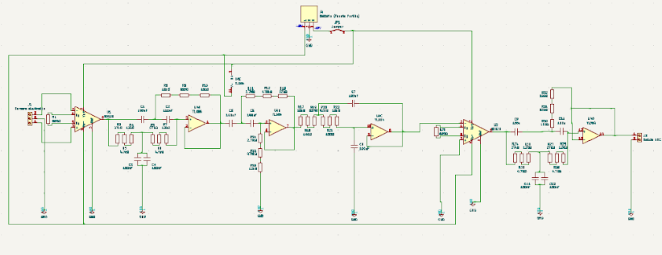
\includegraphics[width=1\linewidth]{Images/Filtros/filtroseeg.png}
    \caption{Esquemático de los filtros del EEG}
\end{figure}

\subsection{Esquemático del sistema de control}
\begin{figure}[H]
    \centering
    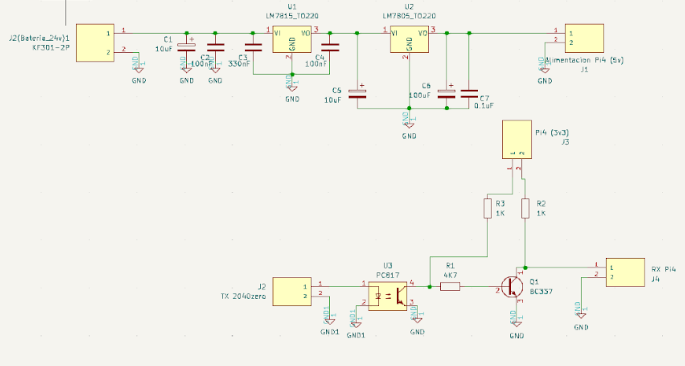
\includegraphics[width=1\linewidth]{Images/SistemaControl/sistemadecontrol.png}
    \caption{Esquemáticos del sistema de control}
\end{figure}

\subsection{Esquemático del sistema Offset}
\begin{figure}[H]
    \centering
    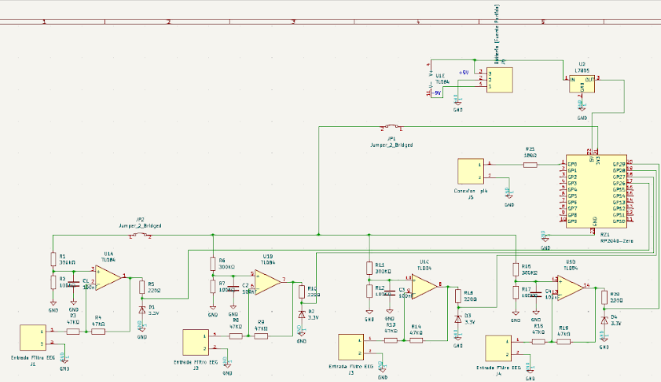
\includegraphics[width=0.95\linewidth]{Images/SistemaOffset/sistemaoffset.png}
    \caption{Esquemático del sistema de Offset}
\end{figure}

\subsection{Esquemáticos de los Puentes H}
\begin{figure}
    \centering
    \includegraphics[width=0.8\linewidth]{Images//PuenteH/Puente-H.jpg}
    \caption{Puente H}
    \label{fig:enter-label}
\end{figure}

\begin{figure}
    \centering
    \includegraphics[width=0.8\linewidth]{Images//PuenteH/PCB-Puente-H.jpg}
    \caption{PCB del Puente H}
    \label{fig:enter-label}
\end{figure}

\subsection{Esquemático del sistema de emergencia}
\begin{figure}[H]
    \centering
    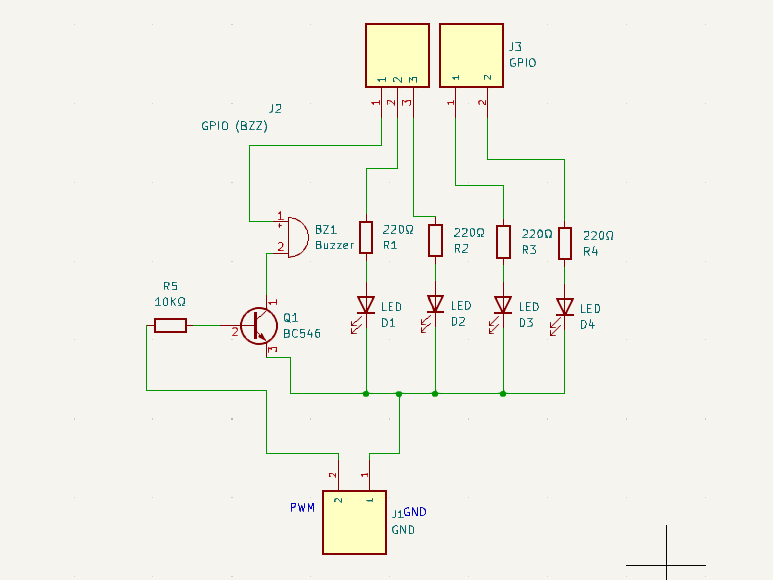
\includegraphics[width=1\textwidth]{Images/SistemaEmergencia/sistemergencia.png}
    \caption{Esquemático del sistema de emegencia}


    \begin{subfigure}[t]{0.5\textwidth}
        \centering
        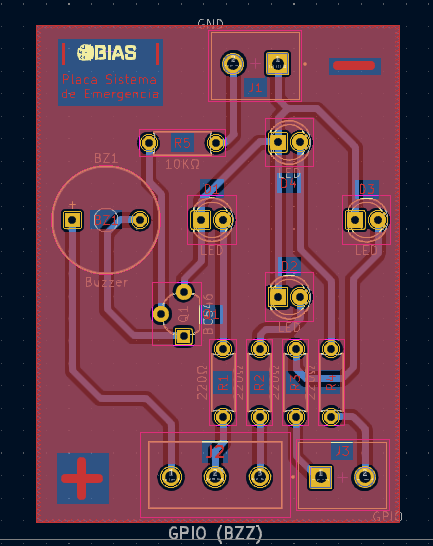
\includegraphics[width=.5\textwidth]{Images/SistemaEmergencia/sistemergenciapcb.png}
        \caption{PCB Del sistema de emergencia}
    \end{subfigure}%
    ~ 
    \begin{subfigure}[t]{0.5\textwidth}
        \centering
        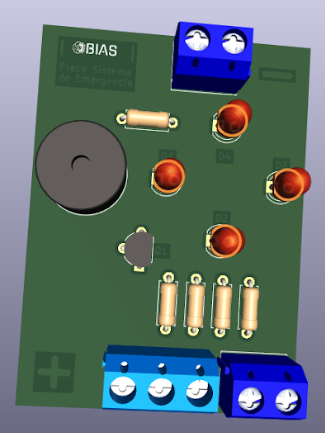
\includegraphics[width=0.5\textwidth]{Images/SistemaEmergencia/sistemergencia3d.png}
        \caption{Modelo 3D Del sistema de emergencia}
    \end{subfigure}

\end{figure}

\subsection{Lista de materiales}
Los programas desarrollados para el proyecto, tales como los filtros digitales, sistemas de inteligencia artificial y otros códigos relacionados, se almacenan en los siguientes dispositivos:

\begin{itemize}
    \item Raspberry Pi 4
    \item RP2040-zero
\end{itemize}

\subsubsection{EEG}
\begin{enumerate}
    \item TL084 (x4)
    \item AD620 (x8)
    \item Capacitores 100nF (x48)
    \item Resistencias 100\Ω (x4)
    \item Resistencias 120\Ω (x16)
    \item Resistencias 560\Ω (x8) 
    \item Resistencias 820\Ω (x16)
    \item Resistencias 1,5k\Ω (x8)
    \item Resistencias 4,7k\Ω (x16)
    \item Resistencias 12k\Ω (x8)
    \item Resistencias 15k\Ω (x8)
    \item Resistencias 27k\Ω (x16)
    \item Resistencias 470k\Ω (x8)
    \item Resistencias 2,7M\Ω (x8)
    \item Electrodos (x9)
\end{enumerate}

\subsubsection{Placa OffSet}
\begin{enumerate}
    \item L7805 (x1)
    \item TL084 (x4)
    \item Jumpers (x2)
    \item Diodos Zenner 3,3V (x4)
    \item Capacitores 100nF (x4)
    \item Resistencias 220\Ω (x4)
    \item Resistencias 50k\Ω (x8)
    \item Resistencias 100k\Ω (x8)
\end{enumerate}

\subsubsection{Sistema de Emergencia}
\begin{enumerate}
    \item Transistor BC546 (x1)
    \item Buzzer 5V (x1)
    \item LEDs Rojos (x4)
    \item Resistencias 220\Ω (x4)
    \item Resistencia 4,7k\Ω (x1)
\end{enumerate}

\subsubsection{Puentes H}
\begin{enumerate}
    \item Transistores IRF4905 (x4)
    \item Transistores IRF2805 (x4)
    \item Optoacopladores PC817 (x4)
    \item Motores 24V 575W (x2)
    \item Resistencias 100\Ω (x4)
    \item Resistencias 180\Ω (x4)
    \item Resistrencias 1k\Ω (x4)
    \item Resistencias 4,7k\Ω (x4)
\end{enumerate}

\subsubsection{Placa reguladora de tensión}
\begin{enumerate}
    \item LM7815 (x1)
    \item Capacitor 100\μF (x1)
    \item Capacitor 330\μF (x1)
    \item Capacitor 470\μF 35V (x1)
    \item Capacitor 470\μF 25V (x1)
\end{enumerate}

\section{Conclusiones}
En esta sección se presentará un análisis detallado de los conocimientos adquiridos a lo largo del desarrollo del proyecto, así como las conclusiones a las que hemos llegado durante este proceso. Se incluirán las conclusiones finales obtenidas, así como una evaluación de las principales limitaciones que afectaron el progreso del trabajo. Además, se ofrecerá un resumen de los resultados alcanzados, destacando los aspectos más relevantes y significativos. Finalmente, se abordarán las perspectivas futuras del proyecto, delineando los pasos a seguir para continuar su desarrollo y mejorarlo en el futuro.

\subsection{Limitaciones}
Durante la ejecución de este proyecto, nos enfrentamos a diversas limitaciones, algunas de las cuales fueron ocasionadas por circunstancias personales de cada integrante del equipo. Como es común en todo proyecto, al principio experimentamos dificultades en la organización y carecíamos de ciertos conocimientos técnicos, los cuales fuimos adquiriendo a lo largo del año.



El tiempo dedicado al proyecto quizá no fue suficiente, considerando la magnitud y la ambición del mismo. Además de estos desafíos iniciales, una de las principales limitaciones fue el prolongado tiempo de espera para obtener los materiales necesarios, los cuales provenían principalmente de la cooperadora. Dado que esta era nuestra principal fuente de herramientas y componentes, nuestro progreso estuvo estrictamente limitado por los tiempos de adquisición manejados por la institución.


Asimismo, al estar creando algo “nuevo”, nos vimos obligados a adoptar un enfoque basado en la prueba y error, ya que la información disponible sobre los temas específicos que requeríamos era escasa. Esta situación también representó un obstáculo significativo, ya que corregir nuestros errores consumió una parte considerable de nuestro tiempo.


Finalmente, al tratarse de un proyecto desarrollado en el ámbito escolar, también nos vimos limitados por el tiempo disponible en la escuela. No pudimos dedicar todo nuestro tiempo al proyecto, ya que debíamos atender otras asignaturas y compromisos académicos.

\subsection{Trabajo Futuro}
El proyecto presenta un alto potencial de rentabilidad en el futuro, sustentado en su carácter innovador y las posibilidades que ofrece su desarrollo continuo. Al tratarse de un invento único en su categoría, se prevé que, con el tiempo y el trabajo adicional necesario, este dispositivo pueda alcanzar un nivel de madurez suficiente para ser comercializado a gran escala.

La inversión en tiempo y recursos adicionales permitirá perfeccionar sus características técnicas, optimizar su funcionalidad, y adaptar el producto a las necesidades de un mercado en expansión. Una vez finalizado y refinado, el proyecto podrá captar la atención de un público más amplio, lo que incrementará su viabilidad comercial y su posicionamiento en el mercado.

En caso de que el desarrollo del proyecto no se complete en su totalidad, este podrá ser aprovechado por la institución educativa, permitiendo que otros grupos de estudiantes continúen su avance. De esta manera, el proyecto no solo servirá como un recurso valioso para futuras generaciones, sino que también fomentará la colaboración y el aprendizaje continuo dentro de la comunidad académica, garantizando su evolución y finalización.

\subsection {Informacion Adicional}
La silla desarrollada en este proyecto es un prototipo, es decir, puede contener fallas de todo tipo, y es sujeto a modificaciones a futuro. Se recomienda su uso siempre acompañado, en zonas amplias libres de obstáculos. No se debe usar en lugares húmedos o si el equipo está mojado, y la inteligencia artificial está adaptada a las muestras de una persona del equipo del proyecto, por lo que para ser usada por alguien mas se deberán muestrear los patrones de movimiento de esta misma.

\subsubsection{Programas Utilizados}
Para el desarrollo del proyecto, hemos requerido hacer uso de los siguientes porogramas, con sus enlaces principales: \newline


    \href{https://github.com/}{-Github}    
    \newline

    \href{https://code.visualstudio.com/}{-Visual Studio Code}
    \newline

    \href{https://thonny.org/}{-Thonny}
    \newline

    \href{https://es.overleaf.com/project}{-Overleaf}
    \newline

    \href{https://www.jetbrains.com/es-es/pycharm/}{-Pycharm}
    \newline

    \href{https://termius.com/}{-Termius}
    \newline

    \href{https://www.kicad.org/}{-Kicad}
    \newline

    \href{https://livewire.laravel.com/}{-Livewire}
    \newline

    \href{https://www.analog.com/en/resources/design-tools-and-calculators/ltspice-simulator.html}{-LTSpice}
    \newline

    \href{https://github.com/apps/desktop}{-GitHub Desktop}

\subsubsection{Agradecimientos}

Queremos expresar nuestro más profundo agradecimiento a los profesores que nos han brindado su invaluable apoyo en la realización de este proyecto:
\begin{itemize}
    \item Fabrizio Carlassara: Su asistencia fue crucial en la programación de la mayor parte del proyecto, así como en la creación de circuitos y esquemáticos, la búsqueda de materiales y el desarrollo de los filtros necesarios.
    \item Sergio Medina: Nos brindó su experiencia en la presentación y comercialización del proyecto, además de colaborar en la programación, la búsqueda de materiales y la planificación de los puentes H.
    \item Carlos Bianco: Su apoyo fue esencial en las pruebas y acondicionamiento de los motores, proporcionándonos herramientas y baterías para dichas pruebas, además de colaborar en la búsqueda de materiales.
    \item Daniel Espósito: Nos proporcionó motores y materiales, además de enseñarnos a construir los puentes H para los motores y nos ayudó a solucionar problemas con las pistas de los circuitos para las altas corrientes.
    \item Federico Solomiewicz: Colaboró principalmente en el desarrollo de los filtros, proporcionándonos herramientas para el proyecto y estando siempre disponible para resolver cualquier duda que surgiera.
    \item Juan Carlos Ruiz: Su colaboración fue esencial en las pruebas de los motores para la silla de ruedas, además de ayudarnos principalmente en la creación de los puentes H para los motores y sus circuitos impresos.
    \item Ana Hartivig: Su ayuda fue imprescindible durante la creacion del EEG. Gracias a ella, pudimos diseñar el EEG, aprendimos como colocar los electrodos y pudimos acceder al hospital El Cruce, Dr. Nestor Kirchner y aprender mas sobre EEGs.
\end{itemize}



\section{Referencias}
En este apartado se presentarán de manera detallada las referencias consultadas al inicio del proyecto, las cuales fueron fundamentales para la conceptualización y desarrollo de la idea final. Estas fuentes proporcionaron el marco teórico y práctico necesario para orientar la dirección del trabajo, influyendo en las decisiones tomadas durante el proceso de diseño y ejecución.

\subsection{Brain Computer Interface}

La primera referencia utilizada en este proyecto es un informe técnico titulado "Brain Computer Interface", escrito por María Madrid Sobrino, el cual aborda el desarrollo de una interfaz cerebro-computadora (BCI) basada en señales EEG, específicamente empleando potenciales evocados visuales de estado estacionario (SSVEP).

Este documento resultó fundamental para nuestra investigación, ya que abarca los siguientes aspectos relevantes:

\begin{itemize}
    \item Introducción a las interfaces cerebro-computadora (BCI): Una interfaz cerebro-computadora (BCI) es un sistema que permite a los usuarios comunicar sus intenciones al entorno externo sin necesidad de utilizar mecanismos fisiológicos naturales, como los nervios periféricos o los músculos. Estas interfaces están diseñadas principalmente para mejorar la comunicación de personas con discapacidades severas, aunque también tienen aplicaciones en la rehabilitación neurológica, en la industria de los videojuegos, entre otros.
    El informe distingue entre dos tipos de BCI: los invasivos, en los cuales los electrodos se implantan directamente en el cerebro, y los no invasivos, donde los electrodos se colocan en la superficie del cráneo. Los BCIs no invasivos, basados en la electroencefalografía (EEG), son los más ampliamente utilizados debido a su practicidad y menor riesgo.

    \item BCI basado en SSVEP: El informe describe un sistema BCI basado en SSVEP (Potenciales Evocados Visuales de Estado Estacionario), que utiliza la respuesta cerebral a estímulos visuales repetitivos. Cuando un estímulo visual parpadea a una frecuencia constante, el cerebro genera señales EEG a la misma frecuencia del estímulo.
    Se destaca la alta efectividad de estos sistemas, que presentan una elevada relación señal-ruido y requieren poco entrenamiento por parte del usuario. Sin embargo, se señala que algunos estímulos visuales pueden provocar fatiga o, en ciertos casos, ataques epilépticos.
\end{itemize}

La referencia detalla el uso de la plataforma BCI2000 para la adquisición de datos, procesamiento de señales y presentación de estímulos. El sistema fue desarrollado empleando C++ y Matlab, lo que permitió la integración de un módulo de procesamiento de señales en Matlab.
El sistema desarrollado incluye una aplicación que presenta 16 opciones visuales organizadas en cuatro grupos, permitiendo al usuario seleccionar una imagen específica enfocando su atención en ella.
El método de clasificación empleado se basa en la frecuencia de los estímulos visuales, y la integración con BCI2000 facilita la ejecución de un sistema de lazo cerrado, donde las señales cerebrales controlan directamente el proceso de selección de imágenes.

Esta referencia fue clave para establecer las bases teóricas y técnicas necesarias para la implementación de un sistema de control basado en señales cerebrales, aplicable a nuestro proyecto de silla de ruedas.

\subsection{Artificial Intelligence for Real-Time Decoding of Motor Commands from ECoG of Disabled Subjects for Chronic Brain-Computer Interfacing}


La segunda referencia utilizada corresponde a la tesis doctoral titulada "Artificial Intelligence for Real-Time Decoding of Motor Commands from ECoG of Disabled Subjects for Chronic Brain-Computer Interfacing", presentada por Maciej Sliwowski en la Université Grenoble Alpes en 2022.

Esta tesis aborda el uso de inteligencia artificial (IA) para la decodificación en tiempo real de comandos motores a partir de señales de electrocorticografía (ECoG) en sujetos con discapacidades motoras. El objetivo principal es mejorar la comunicación y el control mediante interfaces cerebro-computadora (BCI). Los sistemas BCI ofrecen una herramienta de asistencia crucial para pacientes con tetraplejia, proporcionando un medio de interacción directa entre el cerebro y el entorno, compensando la pérdida de funciones motoras.

El enfoque principal del trabajo se centra en los BCI basados en ECoG, que presentan un equilibrio óptimo entre los sistemas intracorticales, más invasivos, y los métodos no invasivos, como el EEG, que suelen ser menos precisos. La tesis estudia específicamente la decodificación de movimientos continuos de traslación de la mano en un paciente tetrapléjico, logrando avances importantes en la interpretación de las señales cerebrales para aplicaciones prácticas en la rehabilitación motora.

Este trabajo es relevante para nuestro proyecto ya que aborda la integración de IA en la interpretación de señales neuronales, lo que resulta fundamental para desarrollar sistemas de control eficientes en tiempo real, como es el caso de nuestra silla de ruedas controlada por la mente. Además, su enfoque en la ECoG aporta perspectivas valiosas para mejorar la precisión y la respuesta del sistema BCI en sujetos con discapacidades motoras severas.

\subsection{Controlled Wheelchair Based on Brain Computer Interface using Neurosky Mindwave Mobile 2}

El artículo presenta el desarrollo de una silla de ruedas controlada mediante una interfaz cerebro-computadora (BCI) utilizando el dispositivo Neurosky Mindwave Mobile 2 para la adquisición de señales EEG. El propósito de este sistema es mejorar la movilidad y la calidad de vida de pacientes post-ictus, permitiéndoles controlar la silla de ruedas a través de sus ondas cerebrales.

Este artículo resultó valioso para nuestras primeras pruebas, dado que inicialmente contábamos con un dispositivo Neurosky Mindwave Mobile 2. Sin embargo, debido a limitaciones en la programación y procesamiento de señales, decidimos descartar esta opción y desarrollar nuestro propio sistema EEG.

El sistema BCI permite a los usuarios controlar dispositivos mediante señales cerebrales, las cuales son registradas utilizando electroencefalografía (EEG). El Neurosky Mindwave Mobile 2 es un dispositivo portátil de bajo costo diseñado para registrar dichas señales EEG. En el contexto de este proyecto, las señales cerebrales se utilizan para controlar una silla de ruedas eléctrica, que originalmente funcionaba a través de un joystick.

El módulo de control del joystick fue reemplazado por un controlador basado en microcontroladores, que procesa las señales cerebrales capturadas y las clasifica utilizando un software desarrollado en Matlab. Este proceso permite que las señales EEG controlen el motor de la silla de ruedas en tiempo real.

En la metodología utilizada se emplea el método de motor imagery, el cual consiste en registrar y analizar las ondas cerebrales asociadas a la imaginación de movimientos motores, tales como caminar o mover las manos. Las señales capturadas por el dispositivo Neurosky se procesan en Matlab y se clasifican en cinco clases de movimiento: avanzar, retroceder, girar a la derecha, girar a la izquierda y una posición neutral.

El sistema incorpora la funcionalidad eSense, una característica del dispositivo que mide los niveles de atención y meditación del usuario, contribuyendo a la precisión del control basado en señales cerebrales.

\subsection{Brain–computer interface for electric wheelchair
based on alpha waves of EEG signal}

El presente estudio aborda el desarrollo de una interfaz cerebro-computadora (Brain-Computer Interface, BCI) destinada al control de una silla de ruedas eléctrica mediante la detección y análisis de ondas alfa generadas por el cerebro, capturadas a través de un electroencefalograma (EEG). El principal objetivo de este sistema es proporcionar asistencia a personas que padecen enfermedades neurológicas graves que afectan severamente su capacidad de movilidad. La solución propuesta destaca por su simplicidad operativa, dado que emplea un número reducido de electrodos y no requiere un extenso período de entrenamiento para los usuarios.

Este estudio fue utilizado como referencia en el desarrollo de nuestro propio proyecto, el cual comparte un enfoque similar en la implementación de un sistema BCI para el control de una silla de ruedas. A partir de la revisión detallada de sus métodos y resultados, adaptamos y optimizamos el diseño de nuestros propios circuitos.

\subsection{A Neural Network Based Brain–Computer Interface for Classification of Movement Related EEG}

La tesis elaborada por Pontus Forslund y presentada en Linköping en diciembre de 2003, trata sobre el diseño de una interfaz cerebro-computadora (BCI) basada en electroencefalografía (EEG), enfocada en la clasificación de movimientos de la mano en dos dimensiones. El objetivo de dicho proyecto es desarrollar un sistema de comunicación intuitivo para individuos con discapacidades motoras graves.

En este estudio, se registraron señales EEG de un sujeto mientras operaba un joystick en cuatro direcciones. Las señales capturadas fueron procesadas mediante un modelo autorregresivo para extraer características relevantes, que luego fueron empleadas como entradas para una red neuronal artificial, diseñada para clasificar la dirección de los movimientos.

Este estudio ha sido utilizado como referencia para nuestro proyecto, específicamente en lo que respecta al reconocimiento de señales EEG y su asignación a los comandos de control del movimiento de la silla de ruedas controlada mediante señales cerebrales.



\section{Lista de códigos}

\subsection{Códigos principales}

\subsubsection{bias.py}
\lstinputlisting[language=python]{Codigos/CodigosPrincipales/bias.py}

\subsubsection{app.py}
\lstinputlisting[language=python]{Codigos/CodigosPrincipales/app.py}

\subsection{Inteligencia artificial}

\subsubsection{bias\_ai.py}
\lstinputlisting[language=python]{Codigos/InteligenciaArtificial/bias_ai.py}

\subsection{Filtrado y procesamiento de señales}

\subsubsection{bias\_dsp.py}

\subsubsection{bias\_dsp\_task.py}

\subsubsection{bias\_graphing.py} 
\lstinputlisting[language=python]{Codigos/Filtrado/bias_graphing.py}

\subsection{Motores}

\subsubsection{bias\_motors.py}
\lstinputlisting[language=python]{Codigos/Motores/bias_motors.py}

\subsection{Recepción de señales}

\subsubsection{bias\_reception.py}
\lstinputlisting[language=python]{Codigos/Recepcion/bias_reception.py}


\subsubsection{CMakeLists.txt}
\lstinputlisting[]{Codigos/Recepcion/CMakeLists.txt}

\subsubsection{pico\_sdk\_import.cmake}
\lstinputlisting[language=c]{Codigos/Recepcion/pico_sdk_import.cmake}

\subsubsection{reception.c}
\lstinputlisting[language=c]{Codigos/Recepcion/reception.c}

\subsection{Página Web}
El sitio web ofrece una breve descripción sobre nosotros, nuestros objetivos, y proporciona enlaces a nuestras redes sociales, donde podrán contactarnos o conocer más acerca de nuestro trabajo.

\begin{center}
    \href{https://proyectobias.github.io/Bias/}{Página Web}
\end{center}

\subsubsection{Lenguaje utilizado en la página web y su código}
El desarrollo de la página web se realizó utilizando los lenguajes HTML y CSS.

Aquí se adjuntan los códigos de la página web:

\begin{center}
    Index.css
\end{center}

\lstinputlisting[language=CSS]{PaginaWeb/index.css}

\begin{center}
    Index.html
\end{center}

\lstinputlisting[language=html]{PaginaWeb/index.html}



\end{document}